\documentclass[a4paper,12pt]{article}
\usepackage[utf8]{inputenc}
\usepackage[ngerman]{babel}
\usepackage{geometry}
\geometry{a4paper, top=2.5cm, bottom=2.5cm, left=2.5cm, right=3cm}
\usepackage{mathptmx}
\usepackage{newtxtext,newtxmath}
\usepackage{setspace}
\usepackage{graphicx}
\usepackage{cite}
\usepackage{url}
\usepackage{setspace}
\onehalfspacing
\bibliographystyle{IEEEtran}
\usepackage[acronym]{glossaries}
\makeglossaries

\usepackage[hypertexnames=false,colorlinks=true,linkcolor=blue]{hyperref}


\usepackage{endnotes}
\usepackage{float} 
\usepackage{booktabs}

\let\footnote=\endnote

\begin{document}
	% Vorderteil: römische Seitenzahlen
	\pagenumbering{roman}
	\thispagestyle{empty}
	
	\begin{center}
		\begin{figure}[h]
			\centering
			\begin{minipage}{0.3\linewidth}
				\centering
				
\includegraphics[width=\linewidth]{Bilder/screenshot017}
				\label{fig:screenshot017}
			\end{minipage}
			\hspace{4cm}
			\begin{minipage}{0.3\linewidth}
				\centering
				
\includegraphics[width=\linewidth]{Bilder/screenshot018}
				\label{fig:screenshot018}
			\end{minipage}
		\end{figure}
		\vspace*{2cm}
		\Huge\textbf{Anomalieerkennung in Keycloak-Logs mittels maschinellen Lernens: Vergleich von Hybridmodellen} \\[1.5cm]
		
		\normalsize
		Vorgelegt von: \\[0.3cm]
		\textbf{Ümmühan Ay} \\
		Matrikelnummer: 7060837 \\[1cm]
		
		Eingereicht am: 24.03.2025 \\[0.3cm]
		Abgabedatum: 08.09.2025 \\[1cm]
		
		Bearbeitungszeitraum: 12 Wochen \\[1cm]
		
		Duale Hochschule Baden-Württemberg Stuttgart\\
		Fakultät für Informatik \\[2cm]
		
		Erstprüfer: Eric Hämmerle \\
		Zweitprüfer: Dr. Janko Dietzsch
		
	\end{center}
	\newpage
	\section*{Danksagung}
	Ich will mich hiermit bei meinem betrieblichen Betreuer Eric Hämmerle bedanken, sowie meinen Vorgesetzten Frithard Meyer von Uptrup, dass diese Arbeit ermöglicht wurde. Ebenfalls bedanke ich mich bei meiner Familie und meine Freunden für die Unterstützung und Motivation, die dazu geführt hat, diese Arbeit fertig zu stellen. Ebenfalls bedanke ich mich bei meinem Betreuer der DHBW, Herr Dr. Janko Dietzsch für das Feedback.
	
	
	\newpage
	\section*{Abstract}
	This thesis examines the implementation and comparison of machine learning models and hybrid architectures for anomaly detection and the detection of intrusion and insider threat attacks in the Keycloak product. The goal was to provide the company with cost-effective tools, as conventional machine learning solutions have been associated with high costs to date. This thesis compares three hybrid models: LSTM autoencoders combined with one of the following algorithms: Isolation Forest, One-Class SVM, and DBSCAN. Previous studies show in particular that LSTM autoencoders in combination with Isolation Forest achieve high results. However, the analyses in this thesis show that the hypothesis cannot be clearly verified or falsified, as LSTM-AE with OCSVM or Isolation Forest achieved comparable overall performance. Log data was used as the data set, which was originally self-generated but ultimately produced by Selenium tests in Keycloak.
	
	
	\newpage
	\section*{Zusammenfassung}
	Diese Arbeit untersucht die Implementierung und den Vergleich von maschinellen Lernmodellen und hybriden Architekturen zur Anomalieerkennung und zur Erkennung von Intrusions- sowie Insider-Threat-Attacken im Produkt Keycloak. Ziel war es, dem Unternehmen kosteneffiziente Werkzeuge bereitzustellen, da konventionelle maschinelle Lernlösungen bisher mit hohen Kosten verbunden sind. In dieser Arbeit wurden drei Hybridmodelle verglichen: LSTM-Autoencoder kombiniert mit jeweils einem der Algorithmen Isolation Forest, One-Class SVM und DBSCAN. Bisherige Studien zeigen insbesondere, dass LSTM-Autoencoder in Kombination mit Isolation Forest hohe Ergebnisse erzielt. Die Analysen dieser Arbeit zeigen jedoch, dass die Hypothese weder eindeutig verifiziert noch falsifiziert werden kann, da LSTM-AE mit OCSVM oder Isolation Forest insgesamt vergleichbare Leistungen erreichten. Als Datensatz wurden Log-Daten verwendet, die ursprünglich selbst generiert, schließlich aber durch Selenium-Tests in Keycloak erzeugt wurden.
	
	\newpage
	\section*{Eigenständigkeitserklärung}
	Hiermit erkläre ich, dass ich die vorliegende Arbeit selbstständig und ohne unzulässige fremde Hilfe angefertigt habe.  
	Alle verwendeten Quellen und Hilfsmittel sind in der Arbeit angegeben.  
	Diese Arbeit wurde bisher keiner anderen Prüfungsbehörde vorgelegt und auch nicht veröffentlicht.
	
		
	\vspace{2cm}
\noindent
Ort, Datum: 25.08.2025 \hspace{3cm}
Unterschrift: \hspace{1cm}
\raisebox{-0.5\height}{
\includegraphics[height=3em]{Bilder/unterschrift}}


	\newpage
	\tableofcontents
	\newpage
	\listoffigures
	\newpage
	\listoftables
	\newpage
	
	\section*{Abkürzungsverzeichnis}
	
	\textbf{ABAC:} Attribute-Based Access Control \\[1em]
	\textbf{AE:} Autoencoder \\[1em]
	\textbf{AUC-PR:} Area Under the Precision and Recall Curve \\[1em]
	\textbf{AUC-ROC:} Area Under the ROC Curve \\[1em]
	\textbf{CVE:} Common Vulnerability and Exposures \\[1em]
	\textbf{CWE:} Common Weakness Enumeration \\[1em]
	\textbf{DBSCAN:} Density-Based Spatial Clustering of Applications with Noise \\[1em]
	\textbf{DGX:} Deep GPU Xceleration \\[1em]
	\textbf{IAM:} Identity und Access Management \\[1em]
	\textbf{IdP:} Identity Provider (Identitätsanbieter) \\[1em]
	\textbf{IF:} Isolation Forest \\[1em]
	\textbf{LSTM:} Long Short Term Memory \\[1em]
	\textbf{MCC:} Matthews Correlation Coefficient \\[1em]
	\textbf{ML:} Machine Learning \\[1em]
	\textbf{NaN:} Not a Number \\[1em]
	\textbf{OCSVM:} One Class Support Vector Machine \\[1em]
	\textbf{OIDC:} OpenID Connect \\[1em]
	\textbf{RBAC:} Role-Based Access Control \\[1em]
	\textbf{RNN:} Recurrent Neural Network \\[1em]
	\textbf{SAML:} Security Assertion Markup Language \\[1em]
	\textbf {SPI:} Serial Peripheral Interface \\[1em]
	\textbf{SSO:} Single-Sign-On \\[1em]
	\textbf {UBA:} User Behavior Analytics \\[1em]
	\textbf {UEBA:} User and Entity Behavior Analytics \\[1em]

	\newpage
	
	\newglossaryentry{abac}{
		name={ABAC},
		description={Zugriffskontrolle basierend auf Benutzerattributen wie Rolle, Standort, Zeit etc}
	}
	
	\newglossaryentry{accesslogs}{
		name={Access Logs},
		description={Protokolle von HTTP-Zugriffen und Statuscodes. Werden häufig auf Webserver- oder Proxy-Ebene erstellt, nicht direkt in Keycloak}
	}
	
	\newglossaryentry{accountsabotage}{
		name={Account Sabotage},
		description={Ein Szenario, in dem ein Benutzer absichtlich Ressourcen löscht, verändert oder auf sie zugreift, um einem System oder einem anderen Benutzer zu schaden}
	}
	
	\newglossaryentry{adam}{
		name={Adam-Optimierer},
		description={Ein adaptiver Optimierungsalgorithmus für neuronale Netze, der den Gradientenabstieg beschleunigt. Er kombiniert die Vorteile von AdaGrad und RMSProp, indem er für jeden Parameter individuelle Lernraten unter Berücksichtigung der ersten und zweiten Momentabschätzung berechnet. Besonders geeignet für große Modelle und Datenmengen}
	}
	
	\newglossaryentry{adminlogs}{
		name={Admin-Logs},
		description={Logs, die administrative Operationen wie CREATE, UPDATE oder DELETE dokumentieren. Enthalten z.\,B. das Feld \textit{operationType}}
	}
	
	\newglossaryentry{adversarialattack}{
		name={Adversarial Attack},
		description={Eine Technik, bei der gezielt manipulative Eingaben erstellt werden, um maschinelle Lernmodelle zu täuschen oder Fehlentscheidungen zu erzwingen. Adversarial Attacks werden häufig in sicherheitskritischen Anwendungen untersucht, um die Robustheit von KI-Systemen gegenüber gezielten Angriffen zu bewerten.}
	}
	
	\newglossaryentry{aucpr}{
		name={AUC-PR},
		description={Area Under the Precision and Recall Curve – misst die Leistung eines Modells im Umgang mit unausgeglichenen Klassen}
	}
	
	\newglossaryentry{aucroc}{
		name={AUC-ROC},
		description={Area Under the Receiver Operating Characteristic Curve – misst die Trennschärfe eines Klassifikationsmodells}
	}
	
	\newglossaryentry{auditlogs}{
		name={Audit-Logs},
		description={Logs zur Nachvollziehbarkeit administrativer Änderungen. In Keycloak Teil der Admin-Logs}
	}
	
	\newglossaryentry{authcodegrant}{
		name={Authorization Code Grant},
		description={OAuth2-Grant-Typ, bei dem der Benutzer über einen Code authentifiziert wird, der vom Client gegen ein Token eingetauscht wird}
	}
	
	\newglossaryentry{authflow}{
		name={Authentication Flow},
		description={Ablauf, der festlegt, wie sich Benutzer oder Clients bei Keycloak authentifizieren}
	}
	
	\newglossaryentry{authType}{
		name=authType,
		description={Ein Attribut in Keycloak-Logs, das angibt, über welchen Mechanismus sich ein Benutzer authentifiziert hat (z.\,B. password, token)}
	}
	
	\newglossaryentry{Autoencoder}{
		name={AE},
		description={Autoencoder – Neuronales Netzwerk zur komprimierten Darstellung und Rekonstruktion von Daten}
	}
	
	\newglossaryentry{backpropagation}{
		name={Backpropagation},
		description={Ein Trainingsalgorithmus für künstliche neuronale Netze, bei dem die Gewichte durch Rückwärtsausbreitung des Fehlers angepasst werden. Dabei wird der Fehler von der Ausgabeschicht zur Eingabeschicht zurückgeleitet, und die Gewichte werden schrittweise gemäß dem Gradientenabstieg verändert. Grundlage für das Lernen in Deep Learning-Modellen}
	}
	
	\newglossaryentry{balancedaccuracy}{
		name={Balanced Accuracy},
		description={Durchschnitt aus Sensitivität (Recall) und Spezifität; besonders geeignet bei unausgeglichenen Klassenverhältnissen}
	}
	
	\newglossaryentry{batchsize}{
		name=Batch-Size,
		description={Die Anzahl an Trainingsbeispielen, die in einem Schritt (Iteration) gleichzeitig durch das neuronale Netz propagiert und zur Gradientenberechnung genutzt werden. Eine kleinere Batch Size führt zu häufigeren Gewichtsanpassungen, während eine größere Batch Size stabilere Gradienten liefert, aber mehr Speicher benötigt}
	}

	\newglossaryentry{bottleneck}{
		name=Bottleneck,
		description={Engste Stelle eines Autoencoders, in der die komprimierte Datenrepräsentation gespeichert wird}
	}
	
	\newglossaryentry{bruteforce}{
		name={Brute-Force-Angriff},
		description={Angriffsmethode, bei der Passwörter oder Zugangsdaten durch systematisches Ausprobieren aller möglichen Kombinationen erraten werden}
	}
	
	\newglossaryentry{client}{
		name={Client},
		description={Anwendung oder Dienst, der Keycloak zur Authentifizierung und Autorisierung verwendet}
	}
	
	\newglossaryentry{clientcredentials}{
		name={Client Credentials Grant},
		description={OAuth2-Grant-Typ, bei dem sich ein Client ohne Benutzerinteraktion authentifiziert}
	}
	
	\newglossaryentry{clientlogin}{
		name={CLIENT LOGIN},
		description={Event-Typ in Keycloak, der bei Anmeldung über einen Drittanbieter-Client (z.\,B. via OAuth2) generiert wird}
	}
	
	\newglossaryentry{clientrole}{
		name=Client-Role,
		description={Client-spezifische Rollen in Keycloak, die Zugriffsrechte innerhalb einer bestimmten Anwendung steuern}
	}
	
	\newglossaryentry{clientscope}{
		name={Client-Scope},
		description={Legt fest, welche Benutzerdaten in ein Token aufgenommen werden, wenn sich ein Benutzer über einen Client authentifiziert}
	}
	
	\newglossaryentry{crud}{
		name=CRUD,
		description={Abkürzung für Create, Read, Update, Delete; beschreibt die grundlegenden Operationen auf Datenbanken oder Entitäten in IT-Systemen}
	}
	
	\newglossaryentry{cve}{
		name={CVE},
		description={Ein öffentliches Verzeichnis bekannter Sicherheitslücken in Soft- und Hardware, das durch eindeutige Identifikationsnummern, Kurzbeschreibungen und betroffene Versionen strukturiert ist}
	}
	
	\newglossaryentry{cwe}{
		name={CPunkte in DBSCAN, die keinem Cluster zugeordnet werden könnenWE},
		description={Ein Katalog von typischen Schwachstellenmustern (Weaknesses), die potenziell zu Sicherheitslücken führen können, z.\,B. unzureichende Authentifizierung oder unsichere Verarbeitung von Daten}
	}
	
	\newglossaryentry{codetotoken}{
		name={CODE TO TOKEN},
		description={Keycloak-Event, das auftritt, wenn ein Authentifizierungscode erfolgreich gegen ein Token eingetauscht wird}
	}
	
	\newglossaryentry{customlogs}{
		name={Custom-Logs},
		description={Benutzerspezifische oder erweiterte Logs, die über Keycloak-Extensions (z.\,B. SPIs) erzeugt werden}
	}
	
	\newglossaryentry{dbscan}{
		name={DBSCAN},
		description={Density-Based Spatial Clustering of Applications with Noise – Clustering-Verfahren für dichte Datenregionen}
	}
	
	\newglossaryentry{ddos}{
		name={DDoS},
		description={Distributed Denial of Service – ein Angriff, bei dem viele Systeme gleichzeitig eine Zielressource mit Anfragen überfluten, um sie unzugänglich zu machen}
	}
	
	\newglossaryentry{decoder}{
		name=Decoder,
		description={Teil eines Autoencoders, der versucht, aus der komprimierten Repräsentation die Originaldaten zu rekonstruieren}
	}
	
	\newglossaryentry{denoising}{
		name=Denoising Autoencoder,
		description={Autoencoder, der lernt, verrauschte Eingaben zu bereinigen und zu rekonstruieren}
	}
	
	\newglossaryentry{dgx}{
		name={DGX},
		description={Deep GPU Xceleration – NVIDIA-Hardwareplattform zur KI-Beschleunigung}
	}
	
	\newglossaryentry{dropoutrate}{
		name={Dropout-Rate},
		description={Der Anteil der Neuronen, die während des Trainings eines neuronalen Netzes zufällig deaktiviert (auf 0 gesetzt) werden, um Überanpassung (Overfitting) zu reduzieren. Eine Dropout-Rate von 0.1 bedeutet, dass 10\% der Neuronen pro Trainingsschritt deaktiviert werden}
	}
		
	\newglossaryentry{encoder}{
		name={Encoder},
		description={Teil eines Autoencoders, der Daten in eine niedrigdimensionale Repräsentation komprimiert}
	}
	
	\newglossaryentry{epochen}{
		name={Epochen},
		description={Ein Begriff aus dem maschinellen Lernen, der die Anzahl der vollständigen Durchläufe über den gesamten Trainingsdatensatz während des Trainings eines neuronalen Netzes bezeichnet. Eine Epoche entspricht einem Zyklus, in dem jedes Trainingsbeispiel einmal verwendet wurde}
	}
	
	\newglossaryentry{eps}{
		name={Eps},
		description={Radius in DBSCAN, der zur Definition der Nachbarschaft eines Punktes dient}
	}
	
	\newglossaryentry{eventlogs}{
		name={Event-Logs},
		description={Protokolle von Benutzer- und Administratoraktionen innerhalb von Keycloak. Enthalten Informationen zu Zeitpunkt, Nutzer-ID, Realm usw}
	}

	\newglossaryentry{eventtype}{
		name={Event-Typ},
		description={Bezeichnet die Art des ausgelösten Ereignisses, z.\,B. LOGIN, LOGOUT, TOKEN\_REFRESH etc}
	}
	
	\newglossaryentry{featurespace}{
		name={Feature Space (Merkmalsraum)},
		description={Der Raum, in dem Datenpunkte durch Merkmale abgebildet werden, häufig hochdimensional}
	}
	
	\newglossaryentry{gamma}{
		name={\(\gamma\)},
		description={Parameter der RBF-Kernel-Funktion bei der One-Class SVM; bestimmt, wie stark ein einzelner Trainingspunkt die Entscheidungsgrenze beeinflusst. Mathematisch tritt \(\gamma\) in der RBF-Kernel-Formel auf: 
			\[
			K(x_i, x_j) = \exp\Big(-\gamma \|x_i - x_j\|^2\Big)
			\] 
			wobei \(x_i, x_j\) Trainingspunkte sind.}
	}
	
	\newglossaryentry{gradientenfluss}{
		name={Gradientenfluss},
		description={Der Gradientenfluss beschreibt die Weiterleitung der Gradienten durch die Schichten eines neuronalen Netzwerks während der Rückwärtspropagation (Backpropagation). Ein stabiler Gradientenfluss ist entscheidend für das erfolgreiche Training tiefer neuronaler Netze. Probleme wie \emph{vanishing gradient} (verschwindende Gradienten) oder \emph{exploding gradient} (explodierende Gradienten) treten auf, wenn der Gradientenfluss über viele Schichten hinweg zu klein bzw. zu groß wird. Der Gradientenfluss ist besonders relevant bei tiefen Netzen wie LSTM- oder GRU-Modellen, da hier die zeitliche Abhängigkeit über viele Zeitschritte die Stabilität der Gradienten stark beeinflussen kann.}
	}
	
	\newglossaryentry{granttype}{
		name={Grant-Type},
		description={Verfahren, mit dem ein Client oder Benutzer bei einem Authentifizierungsserver ein Token anfordert}
	}
	
	\newglossaryentry{hdbscan}{
		name={HDBSCAN},
		description={Hierarchical Density-Based Spatial Clustering of Applications with Noise, eine hierarchische Erweiterung von DBSCAN}
	}
	
	\newglossaryentry{hiddenstate}{
		name={Hidden State},
		description={Interner Zustand eines RNNs, der Informationen über vorherige Zeitschritte speichert}
	}
	
	\newglossaryentry{hybridmodell}{
		name={Hybridmodell},
		description={Ein Modell, das zwei oder mehr unterschiedliche Verfahren kombiniert, z.\,B. LSTM-Autoencoder mit einem klassischen ML-Algorithmus wie Isolation Forest}
	}
	
	\newglossaryentry{iam}{
		name={IAM},
		description={Identity and Access Management – Verwaltung von Identitäten und Zugriffsrechten}
	}
	
	\newglossaryentry{idp}{
		name={Identity Provider},
		description={Externer Anbieter, der Authentifizierungsdienste bereitstellt}
	}
	
	\newglossaryentry{if}{
		name={IF},
		description={Isolation Forest – Verfahren zur Anomalieerkennung durch zufällige Isolation}
	}
	
	\newglossaryentry{impersonate}{
		name={Impersonate},
		description={Ein Event in Keycloak, bei dem ein Administrator die Rolle eines anderen Benutzers übernimmt; wird zur Fehlersuche oder zu Testzwecken verwendet}
	}
	
	\newglossaryentry{insiderthreat}{
		name={Insider Threat},
		description={Sicherheitsbedrohung, die von Personen innerhalb einer Organisation ausgeht,bspw. durch missbräuchliches Verhalten von Mitarbeitenden mit legitimen Zugriffsrechten}
	}
	
	\newglossaryentry{intrusionattack}{
		name={Intrusions-Angriffe},
		description={Angriffe, bei denen ein Angreifer von außen versucht in ein IT-System zu gelangen}
	}
	
	\newglossaryentry{isolationtree}{
		name={Isolation Tree},
		description={Binärer Baum aus dem Isolation Forest-Verfahren zur Isolierung von Datenpunkten}
	}
	
	\newglossaryentry{jbosslogging}{
		name={JBoss Logging},
		description={Logging-API aus dem JBoss-Ökosystem. Bietet eine Abstraktionsschicht über verschiedene Logging-Backends wie log4j, JUL oder slf4j}
	}
	
	\newglossaryentry{jsonl}{
		name={JSONL},
		description={\textit{JSON Lines} (JSONL) ist ein Format, bei dem jede Zeile eine eigenständige JSON-Struktur darstellt. Es eignet sich besonders für große Datenmengen, da jede Zeile unabhängig eingelesen werden kann. Im Gegensatz zu klassischem JSON müssen die Objekte nicht in einer Liste verschachtelt werden; jede Zeile ist ein vollständiges JSON-Objekt.}
	}
	
	\newglossaryentry{jupyternotebook}{
		name={Jupyter Notebook},
		description={Eine interaktive Web-Anwendung, die es ermöglicht, Python-Code auszuführen, Ergebnisse direkt anzuzeigen, Text, Formeln und Visualisierungen zu kombinieren und somit exploratives Programmieren und dokumentiertes Data Science-Arbeiten zu erleichtern}
	}
	
	\newglossaryentry{keras}{
		name={Keras},
		description={Eine hochgradig abstrahierende Deep-Learning-API in Python, die ursprünglich eigenständig entwickelt wurde und heute als offizieller Bestandteil von TensorFlow dient. Keras ermöglicht eine einfache und modulare Modellierung neuronaler Netzwerke}
	}
	
	\newglossaryentry{keycloak}{
		name={Keycloak},
		description={Open-Source Identity-Management-Lösung mit Funktionen wie SSO, RBAC und Brute-Force-Schutz}
	}
	
	\newglossaryentry{kmeans}{
		name={K-Means},
		description={Clustering-Verfahren, das Daten in vordefinierte Cluster basierend auf Mittelwerten aufteilt}
	}
	
	\newglossaryentry{learningrate}{
		name={Learning Rate},
		description={Ein Hyperparameter, der die Schrittgröße bei der Anpassung der Gewichte während des Trainings eines neuronalen Netzes bestimmt. Eine kleinere Lernrate führt zu langsameren, aber stabileren Anpassungen, während eine größere Lernrate schneller, aber instabiler sein kann}
	}
	
	\newglossaryentry{lof}{
		name={LOF},
		description={Local Outlier Factor, ein Verfahren zur Anomalieerkennung über Vergleich lokaler Dichten}
	}
	
	\newglossaryentry{log4j}{
		name={Log4j},
		description={Beliebtes Java-Logging-Framework, bekannt durch seine Flexibilität. Wegen Sicherheitslücken (bspw. Log4Shell) kritisch betrachtet}
	}
	
	\newglossaryentry{logcategory}{
		name={category},
		description={Bezeichnung die Log-Art bzw. den Ereignistypen, z.B. LOGIN}
	}
	
	\newglossaryentry{loginerror}{
		name={LOGIN ERROR},
		description={Event-Typ, der bei einem fehlgeschlagenen Benutzer-Login generiert wird}
	}
	
	\newglossaryentry{loglevel}{
		name={log\_level},
		description={Gibt die Kritikalität oder den Zweck eines Log-Eintrags an (z.\,B. INFO, ERROR, FATAL, DEBUG)}
	}
	
	\newglossaryentry{lstmae}{
		name={LSTM-Autoencoder},
		description={Ein neuronales Netzwerk, das auf Long Short-Term Memory-Zellen basiert, um Sequenzen zu kodieren und zu rekonstruieren, oft zur Anomalieerkennung in Zeitreihen}
	}
	
	\newglossaryentry{lstm}{
		name={LSTM},
		description={Long Short-Term Memory – Neuronales Netz zur Verarbeitung von Sequenzdaten mit Langzeitspeicher}
	}
	
	\newglossaryentry{manageusers}{
		name={manage-users},
		description={Keycloak-Rolle, die es erlaubt, Benutzer in einem Realm zu verwalten (z.\,B. anlegen, bearbeiten, löschen)}
	}
	
	\newglossaryentry{mcc}{
		name={Matthews Correlation Coefficient (MCC)},
		description={Eine robuste Metrik, die alle Werte der Konfusionsmatrix berücksichtigt; besonders geeignet bei unausgeglichenen Datensätzen}
	}
	
	\newglossaryentry{minpts}{
		name={MinPts},
		description={Minimale Anzahl an Punkten innerhalb des Eps-Radius, damit ein Punkt als Kernpunkt eines Clusters gilt}
	}
	
	\newglossaryentry{ml}{
		name={ML},
		description={Machine Learning – Teilgebiet der KI, bei dem Systeme aus Daten lernen}
	}
		
	\newglossaryentry{mse}{
		name={Mean Squared Error (MSE)},
		description={Ein gängiges Fehlermaß zur Bewertung der Modellgüte bei kontinuierlichen Werten. Es berechnet die mittlere quadratische Differenz zwischen den vorhergesagten und den tatsächlichen Werten. Größere Abweichungen werden durch das Quadrieren stärker gewichtet, was das Modell zu präziser Vorhersage zwingt}
	}
	
	\newglossaryentry{nan}{
		name={NaN},
		description={Kein gültiger Zahlenwert}
	}

	\newglossaryentry{noise}{
		name={Noise},
		description={Punkte in DBSCAN, die keinem Cluster zugeordnet werden können}
	}
	
	\newglossaryentry{nu}{
		name={\ensuremath{\nu}},
		description={Parameter der One-Class SVM, der den Anteil an erwarteten Ausreißern im Trainingsdatensatz steuert}
	}
	
	\newglossaryentry{ocsvm}{
		name={OCSVM},
		description={One-Class Support Vector Machine – Algorithmus zur Anomalieerkennung mit einseitiger Klassifikation}
	}
	
	\newglossaryentry{operationtype}{
		name={operationType},
		description={Feld in Admin-Logs, das die Art der Admin-Aktion angibt, z.\,B. CREATE, UPDATE, DELETE oder ACTION}
	}
	
	\newglossaryentry{overfitting}{
		name={Overfitting},
		description={Überanpassung eines Modells an die Trainingsdaten, sodass die Generalisierungsfähigkeit auf unbekannte Daten stark eingeschränkt ist. Typische Indikatoren sind stark abweichende Trainings- und Validierungsfehler. Overfitting tritt häufig bei komplexen Modellen mit zu vielen Parametern oder bei kleinen, nicht repräsentativen Datensätzen auf}
	}
	
	\newglossaryentry{privilegeescalation}{
		name={Privilege Escalation},
		description={Ein Angriffsszenario, bei dem sich ein Benutzer unbefugt höhere Rechte verschafft, z.\,B. um auf administrative Funktionen zuzugreifen}
	}
	
	\newglossaryentry{quarkus}{
		name={Quarkus},
		description={Modernes Java-Framework, optimiert für containerisierte und cloud-native Anwendungen. Ab Keycloak Version 17 als Basisplattform genutzt}
	}
	
	\newglossaryentry{rbac}{
		name={RBAC},
		description={Role-Based Access Control – Zugriffskontrolle auf Basis definierter Rollen}
	}
	
	\newglossaryentry{realm}{
		name={Realm},
		description={Isolierte Umgebung in Keycloak, in der Benutzer, Rollen und Clients separat verwaltet werden}
	}
	
	\newglossaryentry{realmadmin}{
		name={realm-admin},
		description={Eine Administratorrolle in Keycloak, die vollständige administrative Rechte innerhalb eines bestimmten Realms gewährt}
	}
	
	\newglossaryentry{realmrole}{
		name=Realm-Role,
		description={Globale Rollen in Keycloak, die auf alle Clients eines Realms angewendet werden können}
	}
	
	\newglossaryentry{refresh_token}{
		name={Refresh Token},
		description={Ein Refresh Token ist ein kryptografisches Token, das in Authentifizierungssystemen, wie OAuth 2.0, verwendet wird, um ein neues Zugriffstoken (Access Token) zu erhalten, ohne dass sich der Benutzer erneut anmelden muss. Es wird typischerweise mit einer längeren Lebensdauer als das Access Token ausgegeben und ermöglicht die Aufrechterhaltung einer Sitzung über längere Zeiträume, während die Sicherheit durch kürzere Lebensdauer der Access Tokens gewährleistet bleibt.}
	}
	
	\newglossaryentry{rekonstruktionsfehler}{
		name={Rekonstruktionsfehler},
		description={Differenz zwischen Originaldaten und den durch einen Autoencoder rekonstruierten Daten}
	}
	
	\newglossaryentry{rnn}{
		name={RNN},
		description={Recurrent Neural Network – Neuronales Netz zur Verarbeitung zeitabhängiger Daten}
	}
	
	\newglossaryentry{residualblock}{
		name={Residual Block},
		plural=Residual Blocks,
		description={Ein architektonisches Element in tiefen neuronalen Netzwerken, das eine direkte Identitätsverbindung (Shortcut Connection) zwischen Eingabe und Ausgabe eines Layers herstellt. Dadurch lernt das Netzwerk nicht die gesamte Transformation, sondern nur die Differenz (\textit{Residuum}) zur Eingabe. Dies erleichtert die backpropagation und reduziert das Vanishing-Gradient-Problem, wodurch tiefere Netze stabiler trainiert werden können}
	}
	
	\newglossaryentry{scikit}{
		name={Scikit-learn},
		description={Eine weit verbreitete Python-Bibliothek für maschinelles Lernen mit Werkzeugen für Klassifikation, Regression, Clustering und Modellbewertung}
	}
	
	\newglossaryentry{securitylogs}{
		name={Security Logs},
		description={Protokollieren sicherheitsrelevante Ereignisse wie z.\,B. verdächtige Logins, Policy-Verletzungen oder Blockierungen}
	}
	
	\newglossaryentry{selenium}{
		name={Selenium},
		description={Ein Framework zur Automatisierung von Webbrowser-Interaktionen, häufig für Testzwecke genutzt}
	}
	
	\newglossaryentry{serverlogs}{
		name={Server-Logs},
		description={Logs, die Betriebsstatus, Fehler und Debugging-Informationen des Keycloak-Servers dokumentieren}
	}
		
	\newglossaryentry{serviceaccount}{
		name={Service Account},
		description={Konto, das einem Client gehört und ohne Benutzerinteraktion für automatisierte Vorgänge eingesetzt wird}
	}
	
	\newglossaryentry{sequenzlaenge}{
		name={Sequenzlänge},
		description={Die Anzahl aufeinanderfolgender Datenpunkte oder Log-Einträge, die gleichzeitig als Eingabe für ein Modell wie ein LSTM-Autoencoder verwendet werden. Die Wahl der Sequenzlänge beeinflusst, wie viel zeitlicher Kontext das Modell berücksichtigt und kann sich auf die Erkennungsrate von Anomalien auswirken}
	}

	\newglossaryentry{slf4j}{
		name={SLF4J},
		description={Simple Logging Facade for Java – eine Logging-Fassade, die unterschiedliche Logging-Backends wie log4j unterstützt}
	}
	
	\newglossaryentry{spi}{
		name={SPI},
		description={SPI (Service Provider Interface) ist ein Programmier-Schnittstellenkonzept}
	}
	
	\newglossaryentry{spoofing}{
		name={Spoofing},
		description={Täuschungstechniken, bei denen sich ein Angreifer als vertrauenswürdige Instanz ausgibt, um Zugang zu Informationen oder Systemen zu erlangen}
	}
	
	\newglossaryentry{sso}{
		name={SSO},
		description={Single Sign-On – Einmalige Authentifizierung für den Zugriff auf mehrere Anwendungen}
	}
	
	\newglossaryentry{syslog}{
		name={Syslog},
		description={Standardprotokoll zur Übertragung von Logmeldungen in Netzwerkumgebungen, z.\,B. an zentrale Logserver}
	}
	
	\newglossaryentry{tensorflow}{
		name={TensorFlow},
		description={Ein Open-Source-Framework für maschinelles Lernen, entwickelt von Google. TensorFlow bietet eine flexible Infrastruktur zur Definition, Optimierung und Ausführung von Rechenmodellen, insbesondere neuronalen Netzwerken}
	}
	
	\newglossaryentry{timestamp}{
		name={timestamp},
		description={Zeitmarke, zu der ein Event im Log registriert wurde. Wichtige Information für zeitbasierte Analysen}
	}
	
	\newglossaryentry{refreshtoken}{
		name={REFRESH\_TOKEN},
		description={Keycloak-Event-Typ, der beim Aktualisieren eines Zugriffstokens generiert wird}
	}
	
	\newglossaryentry{uba}{
		name={UBA},
		description={User Behavior Analytics – Analyse des Benutzerverhaltens zur Erkennung von Anomalien und Sicherheitsbedrohungen}
	}
	
	\newglossaryentry{ueba}{
		name={UEBA},
		description={User and Entity Behavior Analytics – Verfahren zur Analyse des Verhaltens von Benutzern und technischen Entitäten mit dem Ziel, sicherheitsrelevante Anomalien zu identifizieren}
	}
	
	\newglossaryentry{userlogs}{
		name={User-Logs},
		description={Logs, die Benutzeraktionen ohne Adminrechte erfassen. Typische Eventtypen sind LOGIN, LOGOUT oder TOKEN-Operationen}
	}
	
	\newglossaryentry{vae}{
		name={Variational Autoencoder (VAE)},
		description={Autoencoder-Variante, die Wahrscheinlichkeitsverteilungen in der Bottleneck-Schicht modelliert, häufig für generative Modelle}
	}
	
	\newglossaryentry{vanishing-gradient}{
		name={Vanishing Gradient},
		description={Ein Problem beim Backpropagation-Algorithmus, bei dem die Gradienten beim Durchlaufen vieler Schichten oder Zeitschritte exponentiell kleiner werden. Dies führt dazu, dass frühe Schichten kaum lernen, da ihre Gewichtsanpassungen gegen null gehen. Besonders relevant bei rekurrenten Netzen (RNNs). Lösungsansätze umfassen LSTM-Zellen, Residual-Verbindungen oder geeignete Aktivierungsfunktionen}
	}
	
	\newglossaryentry{viewevents}{
		name={view-events},
		description={Keycloak-Rolle, die es erlaubt, Event-Logs eines Realms einzusehen}
	}
	
	\newglossaryentry{webdriver}{
		name={WebDriver},
		description={Die Komponente von Selenium, die es ermöglicht, Browser programmgesteuert zu steuern}
	}
	
	\newglossaryentry{wildfly}{
		name={WildFly},
		description={Java-Anwendungsserver, früher Basis von Keycloak. Verwendet JBoss Logging und bietet umfangreiche Java EE-Funktionalität}
	}
	
	\newglossaryentry{zerodayangriff}{
		name={Zero-Day-Angriff},
		description={Angriff auf eine bislang unbekannte Sicherheitslücke, für die noch kein Patch existiert}
	}

	\printglossaries 
	\newpage
	\clearpage
	\pagenumbering{arabic}

	\section{Einleitung}
	Laut dem Lagebericht des Bundesamtes für Sicherheit in der Informationstechnik (BSI) 2023 hat die Zahl von Cyberangriffen auf Unternehmen ein bislang nie dagewesenes Niveau erreicht \cite{bsi2023}. Angreifende entwickeln fortlaufend neue Techniken, um bestehende Sicherheitsmechanismen zu umgehen und wirtschaftliche oder strategische Vorteile zu erzielen. Vor diesem Hintergrund stellt sich die zentrale Frage: Wie können Unternehmen potenziell gefährliche Angreifer frühzeitig erkennen, um Schäden effektiv zu verhindern? Die Beantwortung dieser Frage ist essenziell, um die Widerstandsfähigkeit von Informationssystemen gegenüber stetig wachsenden Bedrohungen zu erhöhen.
	
	\subsection{Benutzerverhalten und Anomalien}
	Das Benutzerverhalten umfasst sämtliche Aktionen, Interaktionsmuster und Gewohnheiten einer Benutzers in IT-Systemen. Die Analyse dieser Verhaltensweisen ermöglicht die Identifikation typischer Nutzungsmuster sowie die Erkennung von Abweichungen, die potenziell auf Sicherheitsvorfälle, unautorisierte Zugriffe oder Missbrauch hinweisen können.
	\\[0.5em]
	Anomalien bezeichnen Datenmuster, die signifikant von erwarteten oder üblichen Nutzungsmuster abweichen. Mathematisch gesehen, ist eine Anomalie, ein abweichender Punkt der "normalen"  Bereichen N1 und N2 \cite[S.2]{chandola2009anomaly}. 
	\\[0.5em]
	Neben systemweiten Anomalien – etwa in Netzwerkverkehr oder Gerätezuständen – rücken zunehmend verhaltensbezogene Auffälligkeiten in den Fokus der Forschung. Im Rahmen dieser Arbeit werden Anomalien, die das Benutzerverhalten betreffen, gezielt als \textit{verhaltensbezogene Anomalien} bezeichnet. Sie charakterisieren das individuelle Nutzungsmuster einzelner Anwender innerhalb einer Anwendung oder eines IT-Systems und ermöglichen die Identifikation von Abweichungen, die auf Sicherheitsvorfälle oder Missbrauch hindeuten können.
		
	\subsection{Kategorisierung von Anomalien}
	Nach Chandola et Al. \cite[S.7]{chandola2009anomaly} werden Anomalien in drei Hauptkategorien eingeteilt:
	
	\begin{itemize}
		\item \textbf{Punkt-Anomalien:} Einzelne Dateninstanzen, die im Vergleich zum Großteil der Daten als anomal gelten. Beispiel: Eine Kreditkartentransaktion, deren Betrag deutlich höher ist als die sonst üblichen Ausgaben einer Person.
		\item \textbf{Kontextuelle Anomalien:} Dateninstanzen, die nur in einem spezifischen Kontext als anomal betrachtet werden, ansonsten jedoch normal sind. 
		\item \textbf{Kollektive Anomalien:} Gruppen von Datenpunkten, die zusammen eine Anomalie darstellen, obwohl einzelne Punkte für sich genommen normal erscheinen.
	\end{itemize}
	Dabei umfassen kontextuelle Anomalien zwei Arten von Attributen:
	
	\begin{enumerate}
		\item \textbf{Kontextuelle Attribute:} Bestimmen den Kontext, z. B. geografische Lage oder Zeitstempel.
		\item \textbf{Verhaltensbezogene Attribute:} Beschreiben das tatsächliche Verhalten oder die Charakteristik der Dateninstanz, z. B. die gemessene Temperatur oder der Betrag einer Transaktion.
	\end{enumerate}
	Nach Foorthuis et al. werden Anomalien entsprechend ihrer Merkmale unterschiedlich kategorisiert; sie unterscheiden dabei neun Übertypen \cite{foorthuis2021anomalies}, wobei die Klassifikation auf mathematischen Kriterien basiert. Sanni weist hingegen darauf hin, dass Anomalien im Kontext des Benutzerverhaltens als Abweichungen von üblichen Verhaltensmustern interpretiert werden können \cite[S.3]{Sanni2024}. Damit wird deutlich, dass es sowohl mathematische Kategorisierungen als auch begriffsbasierte, auf reale Anwendungen übertragbare Klassifikationen gibt. Aufgrund der unscharfen Definition des Anomaliebegriffs, der auch außerhalb der Informatik für unterschiedliche Konzepte verwendet wird, ist es erforderlich, für die vorliegende Arbeit eine klar operationalisierte Definition festzulegen.
	\\[0.5em]
	Im Kontext dieser Arbeit wird definiert, dass Anomalien welche sich im Benutzerverhalten äußern, bspw. unter anderem folgende sind:
	
	\begin{itemize}
		\item ungewöhnliche Login-Zeiten,
		\item verdächtige Standorte,
		\item auffällige Rollenprofile,
		\item unübliche Zugriffsrechte,
		\item eine Häufung von Fehlern in der Authentifizierung oder Autorisierung,
		\item Ungewöhnliche IP-Adresse.
	\end{itemize}
	Ein Benutzer, der sich mitten in der Nacht außerhalb der üblichen Geschäftszeiten einloggt, zeigt ein ungewöhnliches Verhalten und weicht somit vom normalen Nutzungsmuster ab- ebenfalls wird davon ausgegangen, dass die meisten Personen eher in der Region arbeiten, wo sie wohnen \footnote{Beleg hier im "Pendleratlas": \url{https://statistik.arbeitsagentur.de/DE/Navigation/Statistiken/Interaktive-Statistiken/Pendleratlas/Pendleratlas-Nav.html}, letzter Zugriff am 28.August.2025}. Moderne Szenarien, wie Homeoffice oder flexible Arbeitszeiten, müssen jedoch berücksichtigt werden: So kann es vorkommen, dass Personen weiter entfernt wohnen oder Entwickler bis spät in die Nacht an einem Projekt arbeiten. Wenn solche Fälle im Unternehmen üblich sind, stellen sie keine Anomalien dar, sondern den Standardbetrieb. Unübliche Zugriffsrechte auf sensible Daten können dagegen Anomalien darstellen, insbesondere wenn ein Benutzer eigentlich keinen Zugriff auf bestimmte Ressourcen haben sollte oder plötzlich mehrere Rollen erhält, die ihm zu viele Rechte einräumen. Häufige Anmelde- oder Autorisierungsfehler können ebenfalls auf \gls{bruteforce}-Angriffe oder andere \gls{intrusionattack}-Versuche hinweisen.
	\\[0.5em]
	Komplexe Abweichungen – etwa Veränderungen in gewohnten Arbeitsabläufen oder zeitlichen Mustern von Datei- und Netzwerkzugriffen – gelten ebenfalls als Anomalien. Ungewöhnliche IP-Adressen können auf unautorisierten Zugriff, \gls{spoofing}-Attacken oder die Nutzung anonymisierender Dienste (z.B. VPN, TOR) hinweisen. Im regulären Betrieb sind IP-Adressen meist geografisch, organisatorisch oder netztechnisch eingeschränkt. Weichen Zugriffe deutlich von bekannten Mustern oder erlaubten Adressräumen ab, kann dies auf externe Angreifer hindeuten. Im Nutzerkontext sind IP-Auffälligkeiten oft ein erstes Signal für Insider-Threat-Attacks oder gestohlene Zugangsdaten.
	\\[0.5em]
	Einige aufgezählten Aspekte sind in \textit{Intrusions-Angriffen} und \textit{\gls{insiderthreat}-Attacks} vorhanden. Intrusionen sind von außen kommende Angriffe,  welche versuchen in das Innere eines Systems zu gelangen, z.B. Brute-Force- Angriffe. Insider-Threat-Attacken können im System selbst schon auftreten, bspw. könnte der Angreifer ein Mitarbeiter im Unternehmen selbst sein.
	\\[0.5em]
	Insider-Threat-Attacks äußern sich nach Legg et Al. \cite[S.2]{legg2015visualizing} in den genannten Aspekten: 
	
	\begin{itemize}
		\item Benutzer zeigt \textbf{abweichendes Verhalten}, z. B.:
		loggt sich deutlich früher ein als üblich
		\item Benutzer zeigt \textbf{bestimmtes Verhalten übermäßig häufig}, z. B. viele Dateien auf einmal herunterladen
		\item Benutzer weist \textbf{neue Attribute oder Aktionen} auf, die zuvor nicht beobachtet wurden, was auf eine \textbf{Insider-Attacke} hindeuten kann
	\end{itemize}
	In dieser Arbeit wird der Begriff verhaltensbezogene Anomalien mit den Erscheinungsformen von Intrusionen und Insider-Threat-Attacks gleichgesetzt, um den Fokus auf sicherheitsrelevante Abweichungen im Nutzerverhalten zu legen. Diese definitorische Vereinfachung ermöglicht eine klare Fokussierung auf sicherheitsrelevante Abweichungen im Nutzerverhalten. Es sei jedoch darauf hingewiesen, dass Anomalien technisch betrachtet als Indikatoren für unterschiedliche Angriffstypen interpretiert werden können.
	
	\subsection{Regelbasierte Methoden und weitere Maßnahmen in \gls{keycloak}}
	Das Unternehmen intension nutzt das Produkt Keycloak \footnote{Siehe die Doku dazu: Keycloak Project: \url{https://www.keycloak.org/}, letzter Zugriff am 28.August.2025}. Dies
	ist ein \gls{iam}-Tool\footnote{IAM steht für \textit{Identity and Access Management} und beschreibt Systeme zur Verwaltung digitaler Identitäten und Zugriffskontrollen}, das unter anderem \gls{sso} (Single Sign-On) bietet\footnote{Single Sign-On ermöglicht einem Nutzer den Zugriff auf mehrere Anwendungen mit nur einer Anmeldung}.
	\\[0.5em]
	Keycloak stellt vorgefertigte Sicherheitsmechanismen zur Verfügung, die größtenteils regelbasiert arbeiten. Solche Maßnahmen definieren explizit, welche Aktivitäten im System erlaubt oder verboten sind. Grundlage dieser Regeln sind meist bekannte Angriffsmuster aus früheren Sicherheitsvorfällen. Zusätzlich bietet Keycloak klassische Zugriffskontrollmechanismen wie \gls{rbac} und \gls{abac}, Brute-Force-Erkennung sowie die Möglichkeit zur Integration externer Netzwerkschutzsysteme wie Firewalls.
	
	\subsection{Grenzen der Sicherheitsmaßnahmen in Keycloak}
	Zwar bietet Keycloak regelbasierte Sicherheitsmaßnahmen an- diese beruhen jedoch größtenteils auf vordefinierten Bedingungen. 
	\\[0.5em]
	Waltl et al. (2017) betonen bspw., dass "regelbasierte Informationsextraktionssysteme (IE)" zwar Vorteile wie Transparenz und Nachvollziehbarkeit bieten, jedoch auch mehrere Einschränkungen aufweisen. Ein wesentlicher Nachteil ist der hohe manuelle Aufwand bei der Erstellung und Pflege der Regeln. Dies führt zu einer begrenzten Flexibilität, da neue oder komplexe Angriffstechniken nur schwer abgebildet werden können. Ein weiteres Problem ist die mangelnde Interoperabilität der Regelsprachen, was die Integration in heterogene Systeme erschwert. Zudem erfordern regelbasierte Systeme oft eine hohe Anzahl an Regeln, um auch geringfügige Variationen in den Eingabedaten zu erfassen, was die Wartung und Erweiterung der Systeme erschwert. Diese Einschränkungen machen regelbasierte Ansätze insbesondere in dynamischen und komplexen Anwendungsbereichen wie der Sicherheitsanalyse weniger geeignet.
	\\[0.5em]
	Neue, bislang unbekannte Angriffsarten (sogenannte \gls{zerodayangriff}e) entziehen sich dieser Logik, da keine entsprechenden Regeln vorliegen. Angreifende nutzen gezielt sogenannte \gls{adversarialattack}s,
	um diese vorhersehbaren Schutzmechanismen zu umgehen. Da die Regeln dieser Systeme häufig offen dokumentiert sind, lassen sich entsprechende Gegenstrategien eher entwickeln.
	\\[0.5em]
	Ein weiteres Beispiel ist der integrierte Brute-Force-Schutz von Keycloak, der jedoch nachweislich umgangen werden kann – etwa durch sogenannte \textit{Timing-Angriffe} \footnote{Genauere Informationen zu Timing-Angriffe im National Vulnerability Database (NVD) unter „CVE-2024-4629 Vulnerability Details“, \url{https://nvd.nist.gov/vuln/detail/CVE-2024-4629}, letzter Zugriff am 28.August.2025}. Dabei analysiert ein Angreifer die Antwortzeit des Systems, um Rückschlüsse auf den Authentifizierungsprozess zu ziehen. Wird beispielsweise ein korrekter Benutzername, aber ein (fast) korrektes Passwort eingegeben, kann die Antwortzeit minimal verlängert sein – was auf die sequentielle Überprüfung der Passwortzeichen hindeutet. Solche zeitlichen Unterschiede im Millisekundenbereich lassen sich mit ausreichend vielen Versuchen systematisch auswerten.
	Auch die Zugriffskontrollmodelle zeigen Schwächen: RBAC wird bei wachsender Komple-
	xität und Vielzahl an Rollen schnell unübersichtlich, während ABAC zwar flexibler ist, dafür jedoch hohen Pflegeaufwand verursacht und anfällig für Fehler ist – insbesondere, wenn viele Attribute aktuell gehalten werden müssen. Zudem lassen sich regelbasierte Systeme durch Taktiken umgehen, die nicht explizit durch die Regeln abgedeckt sind, beispielsweise Social-Engineering-Angriffe. So könnte ein Angreifer versuchen, administrative Rechte zu erlangen, ohne dass das Verhalten gegen eine festgelegte Regel verstößt. Maschinelle Lernmethoden hingegen sind in der Lage, statistische Abweichungen im Verhalten zu erkennen und somit potenziell anomale Aktionen aufzudecken, da sie Wahrscheinlichkeiten und Muster bewerten, anstatt ausschließlich deterministischen Regeln zu folgen.
	\\[0.5em]
	Obwohl für viele Schwachstellen bereits Gegenmaßnahmen existieren, erfordert deren Erkennung und Behebung stets Zeit. Neue Verwundbarkeiten und Sicherheitslücken entstehen kontinuierlich – etwa die Möglichkeit eine Zertifikatsprüfung zu umgehen \footnote{Entdeckt in CVEDetails, „CVE-2025-3501 Details“: \url{https://www.cvedetails.com/cve/CVE-2025-3501}, letzter Zugriff am 28.August.2025}, was jedoch primär netzwerkbasierte Sicherheitslücken betrifft und damit außerhalb des Fokus dieser Arbeit liegt. Diese Beispiele verdeutlichen die aktuellen Grenzen der in Keycloak implementierten Schutzmechanismen.
	\\[0.5em]
	Diese Einschränkungen zeigen, dass regelbasierte Sicherheitsarchitekturen bei der Erkennung komplexer oder neuartiger Bedrohungen an ihre methodischen Grenzen stoßen. Zur Erhöhung der Erkennungsfähigkeit und Flexibilität können daher dynamische, lernfähige Systeme, wie sie durch maschinelles Lernen realisiert werden, eingesetzt werden. Dies bedeutet nicht, dass regelbasierte Methoden an sich unwirksam sind, sondern dass bestehende Sicherheitsansätze ergänzt werden können, um Systeme wie Keycloak weiter abzusichern.
	
	\subsection{Maschinelle Lernmodelle als zukünftige Sicherheitsmaßnahme}
	Die Motivation dieser Arbeit besteht darin, geeignete, hybride, maschinelle Lernmodelle zu identifizieren, welche verhaltensbezogenen Anomalien in den Log-Einträgen (Logs) aus Keycloak erkannt werden können. Maschinelle Lernmodelle stellen heute eine vielversprechende Ergänzung zu klassischen, regelbasierten Sicherheitsmaßnahmen dar, da sie dynamisch auf neue Bedrohungen reagieren können.
	\\[0.5em]
	Im Gegensatz zu statischen Regeln, die lediglich bekannte Muster erfassen, sind \gls{ml}-Modelle in der Lage, aus großen Datenmengen zu lernen und auch unbekannte Anomalien zu identifizieren, die auf potenzielle Angriffe hindeuten. Dadurch sind sie besonders effektiv im Umgang mit Zero-Day-Angriffen oder komplexen, sich ständig wandelnden Bedrohungsszenarien \cite{dahal2025}. Ein weiterer Vorteil ist die Fähigkeit zur kontinuierlichen Anpassung, sodass sich ML-Modelle automatisch auf veränderte Rahmenbedingungen einstellen, ohne dass ein manueller Eingriff notwendig ist.
	\\[0.5em]
	Im Ausblick besteht Interesse daran, das leistungsfähigste Modell in einer Softwarelösung zu verwenden. Zudem spart man Kosten ein, da herkömmliche maschinelle Analysetools häufig mit hohen Lizenzgebühren verbunden sind. Aufgrund datenschutzrechtlicher Vorgaben wurde entschieden, die Keycloak-Logs selbst zu generieren. Dies wird in den Kapiteln 8 und 9 näher erläutert.
	
	\subsection{User (and Entity) Behavior Analytics (U(E)BA)}
	\gls{ueba} ist ein ganzheitlicher Ansatz zur Gewährleistung einer erstklassigen Sicherheit in einem Unternehmen und zur Erkennung von Benutzern, die eine Sicherheitsverletzung im System verursachen könnten. UEBA kann normales und abnormales Verhalten sowohl von Menschen als auch von Computern identifizieren. Die Analyse erfolgt dabei häufig unter Einsatz maschineller Lernverfahren.
	\\[0.5em]
	User and Entity Behavior Analytics (UEBA) stellt eine Weiterentwicklung von User Behavior Analytics (\gls{uba}) dar. Während UBA sich ausschließlich auf das Verhalten von Benutzern konzentriert, berücksichtigt UEBA zusätzlich auch Entitäten wie Server, Anwendungen oder Geräte sowie deren Interaktionen mit den Nutzern.
	\\[0.5em]
	Da sich diese Arbeit auf Keycloak und das Benutzerverhalten im Rahmen von Authentifizierungsprozessen konzentriert, erfolgt keine vollständige Berücksichtigung aller Entitäten oder ihrer Netzwerkbeziehungen.
	\\[0.5em]
	Streng genommen handelt es sich in dieser Arbeit nicht um eine Echtzeit-UBA-Anwendung, da die Auswertung auf bereits gesammelten Logdaten erfolgt. Für die Umsetzung eines \gls{hybridmodell}s in einer produktiven Softwarelösung würde diese Methodik jedoch den Kern einer UBA-Lösung darstellen.
	
	\section{Forschungsstand, Herausforderungen und Hypothesen}
	\subsection{Bisheriger Forschungsstand}
	Die Literatur legt nahe, dass klassische Verfahren wie Isolation Forest (\gls{if}) besonders effektiv in der Anomalieerkennung sind \cite{yan2021extended}. Verfahren wie One-Class SVM (\gls{ocsvm}) erkennen Anomalien teilweise sogar präziser als andere Modelle \cite{arjunan2024comparative}. Auch \gls{dbscan} wird erfolgreich für die Cluster-basierte Anomalieerkennung eingesetzt, wobei "multiple Parameter" zur Optimierung verwendet werden \cite{thang2011dbscan}. 
	\\[0.5em]
	Für sequenzielle Daten wie Zeitreihen oder Nutzerinteraktionen zeigen neuronale Netze, insbesondere Long Short-Term Memory (\gls{lstm}) und Autoencoder (\gls{Autoencoder}), signifikante Vorteile, da sie zeitliche Abhängigkeiten und komplexe Muster besser erfassen können und teilweise andere Modelle wie TimeGPT übertreffen \cite{demir2024comparative}. Zur Erkennung von Intrusionen und "benutzerbasierten Anomalien" eignet sich ein LSTM-AE gut \cite{Iseed2025}.
	\\[0.5em]
	Hybridmodelle, also Ansätze, bei denen mehrere Algorithmen und/oder neuronale Netze kombiniert werden, zeigen ebenfalls vielversprechende Ergebnisse:
	\\[0.5em]
	Aus der Literatur ergibt sich, dass Kombinationen aus LSTM und Autoencoder als besonders robust und effektiv gelten – etwa in Szenarien zur Luftqualitätsüberwachung, mit einer Genauigkeit von 99,5\,\% \cite{wei2023lstm}.
	\\[0.5em]
	Andere Studien zeigen, dass sich LSTM-AE in Kombination mit IF zu einem leistungsfähigen Modell zur Anomalieerkennung entwickeln lässt, das ebenfalls hohe Genauigkeiten erzielt \cite{tran2020lstm_if}. Weitere Arbeiten, wie die von Ghrib et al. \cite{ghrib2020hybrid}, untersuchen hybride Ansätze unter Verwendung von IF: Es hat eine geringere Rechenkomplexität. Zudem weisen Hybridmodelle mit IF eine hohe Effektivität bei der Erkennung von Intrusionen auf \cite{marteau2017hif}.
	\\[0.5em]
	Eine Studie von Ergen et al. \cite{ergen2017unsupervised} zeigt, dass die Kombination von LSTM-basierten Architekturen mit OCSVM zu signifikant verbesserten Erkennungsraten bei der Anomalieerkennung führt – insbesondere bei sequenziellen Daten. In einer weiteren Studie wird LSTM mit AE und OCSVM kombiniert, und Explainable AI wird genutzt, um Intrusionen zu erkennen, wobei ebenfalls sehr gute Ergebnisse erzielt werden \cite{ha2022explainable}.
	\\[0.5em]
	Zhou et al. zeigen, dass im IoT-Bereich eine Kombination von LSTM-AE und DBSCAN unnormale Temperaturen deutlich besser erkennen kann \cite{zhou2024improved}. Eine weitere Studie demonstriert, dass auch DBSCAN in Kombination mit AE Intrusionen sehr effektiv erkennen kann \cite{prabu2024dbscan}.
	\\[0.5em]
	Die Literatur zeigt jedoch auch potenzielle Schwächen der genannten Netzwerke und Modelle. LSTM- und Autoencoder-Modelle sind anfällig für \gls{overfitting} und benötigen große Datenmengen \cite{liu2019ensemble}.
	\\[0.5em]
	Isolation Forest und OCSVM sind oft sensitiv gegenüber der Wahl der Parameter und muss je nach Architektur angepasst werden, wie auch in einer Studie nach Chua et Al. diskutiert wurde \cite{chua2024web}. DBSCAN ist ebenfalls sehr empfindlich gegenüber der Wahl von Parametern wie \gls{eps} und \gls{minpts}, erkennt Cluster mit unterschiedlicher Dichte nur schlecht und kann bei hohem Rauschen versagen \cite{ahmadzadeh2025graphdbscan}.
	\\[0.5em]
	Hybridmodelle haben ebenfalls ihre Schwächen: Zwar verbessern sie häufig die Leistung, gleichzeitig erschwert ihre Komplexität die Interpretierbarkeit und den Einsatz in Echtzeitanwendungen \cite{Moussaoui2025}.
	\\[0.5em]
	Insgesamt zeigt sich, dass hybride Ansätze dieser Verfahren dennoch vorteilhaft sind, um die Herausforderungen bei der Erkennung verhaltensbezogener Anomalien in realen Anwendungen effizient zu bewältigen. Die betrachteten Arbeiten betonen zudem unterschiedliche Anomalie-Typen, für die jeweiligen Modelle eingesetzt werden. 
	
	\subsection{Hypothese}
	Um die Forschung zu vertiefen, soll gezielt untersucht werden, wie verschiedene Hybridmodelle zur Erkennung verhaltensbezogener Anomalien, Intrusionen und Insider-Threat-Angriffe eingesetzt werden können.
	\\[0.5em]
	Basierend auf der Literatur besteht daher Interesse an einem umfassenden Vergleich zwischen Hybridmodellen aus LSTM-AE und den weiteren genannten klassischen maschinellen Lernalgorithmen sowie an einem Vergleich dieser Modelle einzeln.
	\\[0.5em]
	Daraus wurde folgende Hypothese abgeleitet:
	\\[0.5em]
	\textit{Es wird erwartet, dass der \gls{lstmae} in Kombination mit Isolation Forest unter unterschiedlichen \gls{sequenzlaenge}n höhere Ergebnisse in den Metriken F1-Score, Balanced Accuracy und MCC erzielt als die Kombinationen des LSTM-Autoencoders mit DBSCAN bzw. OCSVM.}
	\\[0.5em]
	Die zugehörige Nullhypothese lautet:
	\\[0.5em]
	\textit{Unter verschiedenen Sequenzlängen zeigt der LSTM-Autoencoder in Kombination mit Isolation Forest keine höheren Ergebnisse in den Metriken F1-Score, Balanced Accuracy und MCC als die Kombinationen mit DBSCAN oder OCSVM.}
	\\[0.5em]
	Folgende Hybridmodelle werden also implementiert:
	\begin{itemize}
		\item LSTM-AE und Isolation Forest
		\item LSTM-AE und One-Class SVM
		\item LSTM-AE und DBSCAN
	\end{itemize}
	Dabei wird ein Keycloak-Datensatz verwendet, welches von den Modellen analysiert wird. 
	\\[0.5em]
	Die Sequenzlänge wird als unabhängige Variable untersucht, da sie die Stabilität und Genauigkeit der Modellvorhersagen beeinflussen kann - der Fokus auf dem besten Modell in dieser Arbeit zeigt sich durch seine Stabilität und Genauigkeit. Mit verschiedenen Metriken wird geprüft, welches Modell hinsichtlich Klassifikationsgenauigkeit und Konsistenz die besten Ergebnisse erzielt. 
	\\[0.5em]
	Unter Konsistenz wird verstanden, welches Modell nicht zufällig, sondern anhand eines stabilen Algorithmus klassifiziert- die Bewertung dieser Eigenschaft erfolgt durch die Messung des \gls{mcc}.
	\\[0.5em]
	Die Klassifikationsgenauigkeit gibt an, wie oft korrekt Anomalien erkannt wurden und weist auf eine geringe False-Prositive und False-Negative Rate hin, die sich mit dem F1-Score und auch der \gls{balancedaccuracy} messen lässt. Auf die genannten Metriken wird in Kapitel 3 nochmals genauer eingegangen.
	\\[0.5em]
	Die Hypothese, dass LSTM-Autoencoder (LSTM-AE) in Kombination mit Isolation Forest (IF) besonders effektiv ist, stützt sich auf die komplementären Stärken beider Methoden. LSTM-AE kann zeitabhängige Muster im Benutzerverhalten erfassen und Unterschiede zwischen normalem und anomalem Verhalten über Rekonstruktionsfehler erkennen. Zudem wird angenommen, dass Isolation Forest als einzelnes Modell effizienter Anomalien erkennen kontte als OCSVM und DBSCAN \cite{Lu2025}. Ziel ist es, zu prüfen, ob diese Robustheit auch bestehen bleibt, wenn Isolation Forest mit einem LSTM-AE kombiniert wird- und unter welchen Sequenzlängen.
	\\[0.5em]
	Zusätzlich wurden die Einzelmodelle Isolation Forest, OCSVM und DBSCAN auf den Keycloak-Daten explorativ angewendet. Diese Evaluation ist nicht Bestandteil der zentralen Vergleichsstudie, dient jedoch als Ergänzung zur Einordnung der Ergebnisse der Hybridmodelle.
	\\[0.5em]
	Sie ermöglicht einen informellen Eindruck davon, wie sich gängige Einzelverfahren im gegebenen Kontext verhalten, ohne dass daraus direkte Schlussfolgerungen im Sinne der zentralen Forschungsfrage abgeleitet werden. Zudem kann so geprüft werden, ob komplexere Architekturen eventuell auch Nachteile haben und einfache Modelle unter bestimmten Bedingungen überlegen sind.
	\\[0.5em]
	Die Kombination von Hybridmodellen mit zwei verbundenen Netzwerken und drei klassischen Lernalgorithmen bietet einen interessanten Vergleich, auch wenn der Vergleich zwischen den Modellen als unausgeglichen wahrgenommen werden kann. Es wird jeweils das Hybridmodell LSTM-AE mit einem der drei Lernalgorithmen kombiniert und miteinander verglichen.
	\\[0.5em]
	Tran et al. zeigen beispielsweise bereits, dass ein Vergleich von LSTM-AE mit OCSVM bspw. durchgeführt wurde und dass das Hybridmodell LSTM-AE Anomalien präziser einteilen konnte \cite{tran2021forecasting}. Daher erscheint ein erweiterter Vergleich zwischen komplexeren Hybridmodellen, die noch klassische Lernalgorithmen verwenden, und den einfachen Algorithmen sinnvoll.
	\\[0.5em]
	Zudem werden komplexere Daten verwendet, nämlich Logdaten, die Aufschluss über das Benutzerverhalten geben und keine vorgefertigten Datensätze, wie sie in den erwähnten Studien beschrieben sind.
	\\[0.5em]
	Der Vergleich trägt somit dazu bei, bisherige Studien zu ergänzen und einen neuen wissenschaftlichen Mehrwert zu schaffen, indem komplexe Hybridmodelle miteinander verglichen werden.
	
	\section{Methoden und Störfaktoren}
	\subsection{Metriken}
	Typischen Verfahren wie die Berechnung der Precision, des Recall und F1-Score werden angewandt. Die Metriken folgen alle unterschiedlichen:
	\\[0.5em]
	\textbf{Accuracy} = \(\frac{TP + TN}{TP + TN + FP + FN}\) gibt den Anteil korrekt klassifizierter Beispiele an allen Beispielen an.
	\\[0.5em]
	\textbf{Precision} = \(\frac{TP}{TP + FP}\) misst den Anteil korrekt als positiv klassifizierter Beispiele an allen als positiv vorhergesagten. 
	\\[0.5em]
	\textbf{Recall} = \(\frac{TP}{TP + FN}\) zeigt, wie viele der tatsächlichen Positiven korrekt erkannt wurden. 
	\\[0.5em]
	\textbf{F1-Score} = \(2 \times \frac{\text{Precision} \times \text{Recall}}{\text{Precision} + \text{Recall}}\) ist das harmonische Mittel von Precision und Recall. 
	\\[0.5em]
	Dabei stehen TP, TN, FP, FN für True-Positives, True-Negatives, False-Positives und False-Negatives.
	\\[0.5em]
	Bei der Auswahl der Metriken muss man einige bekannte Probleme betrachten:
	\\[0.5em]
	Eine Studie weist aber daraufhin, dass des Öfteren diese Metrik angewandt wird und oft nicht valide Begründungen für die Klassifikationsgenauigkeit des Modells bietet. U.a. wies diese Studie daraufhin, dass ein Großteil, der Studien nur anhand der Accuracy der maschinellen Lernmodelle ihre Effizienz misst und andere Eigenschaften ausblenden \cite{provost1998case}. 
	\\[0.5em]
	Zudem wird hingewiesen, dass durch stark unausgewogenen Klassen die Accuracy irreführend ist. Dies liegt daran, weil die Accuracy nur angibt, wie viele Datenpunkte richtig klassifiziert wurden. Wenn aber die Klassen unausgeglichen sind (z.B. 99\,\% der Datenpunkte gehören Klasse A der Rest zu Klasse B), ist es wahrscheinlicher, dass das Modell sich immer nur entweder für Klasse A oder Klasse B entscheidet- da es mehr Objekte von Klasse A gibt- diese dahin zu klassifizieren, obwohl es noch eine kleinere Klasse B gab, die aber nicht berücksichtigt wurde. Es wird dann zwar eine hohe gute Accuracy von 99\,\% erreicht, was aber bedeutet, dass 1\,\%, die von Klasse B ebenfalls zu Klasse A zugeordnet wurden. Dies nennt man auch Accuracy Paradoxon. Um dieses Parodoxon zu vermeiden, will man in dieser Arbeit Metriken einsetzen, welche ausschlaggebender sind. 
	\\[0.5em]
	Dies bedeutet nicht, dass die Accuracy keine Aussagekraft bei der Bewertung der Modelle besitzt. Vielmehr ist sie eine häufig verwendete Metrik, während andere, effizientere Bewertungsmethoden, die sich insbesondere für unausgeglichene Datensätze eignen, oftmals unberücksichtigt bleiben. Die gleichzeitige Verwendung einer Vielzahl weiterer Metriken wäre in diesem Kontext jedoch übermäßig und würde den Fokus der Analyse verwässern.
	\\[0.5em]
	Es muss ebenfalls erwartet werden, dass es in dieser Arbeit zu einem Klassenungleichgewicht kommen kann, da Anomalien in den Testdaten sehr wenig auftreten, wie es in der Realität erwartet wird. Die Literatur zeigt, dass die Auswirkungen dieses Ungleichgewichts relativ sind und je nach eingesetztem Lernalgorithmus und Datensituation variieren \cite{japkowicz2002systematic}. 
	\\[0.5em]
	Fourure et al. weisen darauf hin, dass der Fokus in vielen Studien häufig auf dem F1-Score liegt. Dieser ist jedoch stark abhängig von der Wahl des Evaluationsprotokolls, etwa der Kontaminationsrate oder des Schwellenwerts, wodurch er künstlich erhöht werden kann und keine tiefgehenden oder verlässlichen Aussagen über die Modellleistung liefert \cite{fourure2021anomaly}. Es wird kritisiert, dass dieser zwar eine gute Gewichtung zwischen Precision und Recall zeigt, jedoch an sich nicht genau angeben kann, ob nun wirkliche das Modell Probleme in False-Positive-Klassifizierungen oder False-Negative-Klassifizierungen hat.
	\\[0.5em]
	Eine weitere Untersuchung von Fourure et al. zeigt, dass in vielen Vergleichsstudien auch wie zuvor erwähnt die Accuracy oder dem F1-Score betrachtet wird, während andere wichtige Metriken oft vernachlässigt bleiben. Zudem zeigen Sie, dass durch die Auswahl bestimmter Trainings- und Testdatensätze kann der F1-Score künstlich erhöht werden, was zu einer verzerrten Einschätzung der Modellleistung führt \cite{fourure2021anomaly}.
	\\[0.5em]
	Insgesamt lässt sich festhalten, dass jede Metrik individuelle Stärken und Schwächen besitzt. Gleichzeitig wird kritisiert, dass viele Studien auf Metriken zurückgreifen, die nicht ausreichend aussagekräftig sind.
	\\[0.5em]
	Generell ist die Kritik, dass nur ein einfacher Prozentsatz nicht ausschlaggebend für die Fähigkeiten des Modells ist - dennoch werden diese als übliche Metriken angewandt. Um Störfaktoren der üblichen Metriken noch zusätzlich zu verringern, werden modernere Metriken angewandt:
	
	\begin{itemize}
		\item \textbf{Area Under the ROC Curve (\gls{aucroc})}:Diese Kurve zeigt, wie sich die True-Positive-Rate und False-Positive-Rate bei verschiedenen Schwellenwerten verändern. Für jeden Schwellenwert kann man ablesen, wie viele False Positives bzw. False Negatives entstehen. Die AUC-ROC fasst die Performance über alle Schwellenwerte zusammen.
		\item \textbf{Area Under the Precision-Recall Curve (\gls{aucpr}:)} Diese Kurve zeigt die Beziehung zwischen Precision und Recall bei verschiedenen Schwellenwerten. Für jeden Schwellenwert misst man neu, wie genau (Precision) und wie vollständig (Recall) die positiven Fälle erkannt werden. So erkennt man, bei welchem Schwellenwert die Balance zwischen Precision und Recall am besten ist.
		\item \textbf{Matthews Correlation Coefficient (\gls{mcc}):} Eine umfassende Metrik, die alle vier Werte der Verwirrungsmatrix (True Positives, True Negatives, False Positives, False Negatives) berücksichtigt. MCC liefert einen Wert zwischen -1 und 1, wobei 1 perfekte Vorhersage, 0 zufällige Vorhersage und -1 vollständig falsche Vorhersage bedeutet. Besonders geeignet für unausgeglichene Datensätze.
		\item \textbf{\gls{balancedaccuracy}:} Der Anteil der negativen Beispiele, die fälschlicherweise als positiv klassifiziert wurden. Sie wird berechnet als \(\text{FPR} = \frac{\text{False Positives}}{\text{False Positives} + \text{True Negatives}}\) und ist wichtig, um die Fehlerquote bei der Erkennung negativer Fälle zu bewerten.
	\end{itemize}
	Auch wenn diese Metriken  mehr Informationen über die Verarbeitungsweise der Modelle schließen lassen, haben diese ebenfalls Einschränkungen. Davis und Goadrich zeigen, dass ROC und PR Kurven durch eine eindeutige mathematische Beziehung miteinander verbunden sind. Fuer ein gegebenes Datenset enthalten beide Kurven die gleichen Informationen, werden aber unterschiedlich dargestellt. \cite{davis2006relationship}.
	\\[0.5em]
	Studien zeigen, dass alternative Metriken wie MCC und Balanced Accuracy insbesondere bei unausgeglichenen Datensaetzen vernuenftige Eigenschaften aufweisen. Chicco und Jurman zeigen, dass MCC im Vergleich zu Accuracy und F1 Score robustere und wahrheitsgetreuere Ergebnisse liefert. Brodersen et al. zeigen, dass Balanced Accuracy durch die gleichgewichtete Beruecksichtigung beider Klassen Verzerrungen bei unbalancierten Klassen vermeidet \cite{chicco2020advantages, brodersen2010balanced}.
	\\[0.5em]
	Außer diesen Metriken wurde noch überlegt, einen sogenannten Cross-Validation-Test durchzuführen. Cross-Validation \footnote{Erklärung der Modellbewertung: \url{https://scikit-learn.org/stable/modules/cross\_validation.html}, letzter Zugriff am 28.August.2025} ist keine Metrik wie z.B. der F1-Score, sondern eine Methode zur Modellbewertung. Sie unterteilt dabei den Datensatz in \textit{k} gleich große Teile. Das Modell wird dann k-mal trainiert, jedes mal mit k-1 Teilen als Trainingsdaten. Der übrig gebliebene Teil wird als Testdatensatz und Validierungsdatensatz verwendet. Der Sinn dahinter ist die Trainingsdaten so zu verteilen, dass das Modell jedes mal neu trainiert wird. Dies soll Overfitting auf den Daten vermeiden. Zudem soll sie die Ergebnisse nach jedem Training des k-Datensatzes zeigen, damit sich erkennen lässt, ob es an bestimmten Stellen Abweichungen gab. Dieser wurde jedoch verworfen, um die Auswertung und wissenschaftlichen Test an einer anderen Art der Bewertung zu verwenden, welche eher üblich ist in wissenschaftlichen Arbeiten.
	
	\subsection{Störfaktoren}
	Für einen objektiven Vergleich der Modelle ist insbesondere die Art der Datenvorverarbeitung entscheidend. Alle Features in den Logs werden numerisch verarbeitet; jedoch ist nicht bekannt, welche Features das Lernverhalten der Modelle maßgeblich beeinflussen. Eine sorgfältige Vorverarbeitung ist daher notwendig, um sicherzustellen, dass alle relevanten Features, korrekt berücksichtigt werden.
	\\[0.5em]
	Ein weiterer wesentlicher Faktor ist die Wahl der Modellparameter. Parameter wie beispielsweise die Anzahl der \gls{epochen} oder die Gesamtarchitektur können das Verhalten und die Ergebnisse der Modelle erheblich beeinflussen. Die einzelnen Algorithmen wie IF reagieren sensibel auf Parameter-Änderungen und dass die Ergebnisse dadurch erheblich beeinflusst werden. Dementsprechend muss man vorsichtig sein und gewährleisten, keine unangemessen Parameter zu setzen und dafür zu sorgen, dass trotz der Setzung einer fairer Vergleich ermöglicht wird.
	\\[0.5em]
	Die Zufälligkeit der Daten beeinflusst ebenfalls die Modellleistung. Die Datensätze müssen einerseits zufällig generiert sein, gleichzeitig aber einen kontinuierlichen Zusammenhang aufweisen, wie er bei realen Cyberangriffen vorkommt. Dies ist insbesondere für LSTM-Netzwerke relevant, die auf sequenzielle Abhängigkeiten angewiesen sind. Kontextlose oder stark fragmentierte Datenpunkte könnten das Lernen solcher Modelle erschweren. Von daher werden Ergebnisse mit einer hohen False-Positive-Rate erwartet.
	\\[0.5em]
	Auch die verfügbare Rechenleistung kann die Verarbeitungsgenauigkeit beeinflussen. Zu kurze oder zu lange Trainingszeiten sowie eine hohe Rechenintensität wirken sich negativ auf die Modellleistung aus. Daher werden in allen Modellen Regulierungstechniken \footnote{Definition unter: \url{https://www.sciencedirect.com/topics/engineering/regularization}, letzter Zugriff am 28.August.2025} implementiert, um eine ausgewogene Trainingsdauer und Leistungsfähigkeit zu gewährleisten.
	\\[0.5em]
	Der Aufbau der zu verarbeitenden Daten ist ein weiterer entscheidender Faktor. Bei teilweise synthetisch generierten Logs bestimmt der Anteil der als anomal gekennzeichneten Zeilen die Bewertung der Modelle.
	\\[0.5em]
	Die Generierung synthetischer Logs bringt methodische Herausforderungen mit sich. Alternativ wurden auch reale Daten in Betracht gezogen, etwa durch automatisierte Tests oder firmeninterne Logs. Wie bereits in Kapitel 2 erläutert ist die Benutzung von Unternehmensdaten aufgrund den datenschutzrechtlichen Herausforderungen nicht machbar. Diese entsprechen nicht exakt dem realen Benutzerverhalten, was die Aussage der Hypothese etwas beschränkt auf die für den Vergleich genutzten generierten Daten. Ein Vorteil ist jedoch, dass sich der Aufbau und die Struktur hierfür kontrollieren lassen.
	\\[0.5em]
	Acikmese und Alptekin beschreiben, dass LSTM Modelle in ihrem Experiment als datenhungrig erscheinen, da die geringe Datengröße nicht ausreichte, um eine gute Generalisierung zu erreichen \cite{Acikmese2019}. Ein kleiner Datensatz kann zu einer Unterforderung des Modells führen und die Ergebnisse signifikant beeinflussen. Auch in dieser Arbeit ist dies zu berücksichtigen.
	\\[0.5em]
	Beim Vergleich der Modellleistungen mit synthetischen und realen Daten ist zu erwarten, dass die Ergebnisse variieren, da sich die Feature-Struktur und die logische Beschaffenheit der Logs zwischen den Datensätzen unterscheiden.
	
	\section{Angewandte Technologien}
	\subsection{\gls{scikit} Learn}
	Scikit-learn\footnote{Mehr Informationen zu Scikit sind hier nachzulesen: \url{https://scikit-learn.org/stable/}, letzter Zugriff am 28.August.2025}
	ist eine weitverbreitete Open-Source-Bibliothek für maschinelles Lernen in Python. Sie stellt eine Vielzahl von Werkzeugen für klassische Machine-Learning-Aufgaben bereit, darunter Klassifikation, Regression und Clustering sowie Modellbewertung und -selektion. Scikit-learn bietet eine Reihe vorimplementierter Modelle wie IF, OSCVM und DBSCAN.
	
	\subsection{Keras}
	\gls{keras}\footnote{Offizielle Dokumentationzu Keras ist verfügbar unter: \url{https://keras.io/}, letzter Zugriff am 28.August.2025} ist eine benutzerfreundliche, modulare und erweiterbare Open-Source-Bibliothek für die Entwicklung von Deep-Learning-Modellen in Python. Sie bietet eine einfache und intuitive API, die die schnelle Implementierung und das Training neuronaler Netze ermöglicht. Keras unterstützt verschiedene neuronale Netzwerkarchitekturen, darunter Convolutional Neural Networks (CNNs), Recurrent Neural Networks (\gls{rnn}s) und AE's.
	
	\subsection{\gls{tensorflow}}
	TensorFlow\footnote{TensorFlows offizielle Dokumentation ist verfügbar unter: \url{https://www.tensorflow.org/}, letzter Zugriff am 28.August.2025} ist ein umfangreiches Open-Source-Framework von Google für maschinelles Lernen und Deep Learning. Es ermöglicht die effiziente Definition, Optimierung und Ausführung von numerischen Berechnungen. TensorFlow bietet Skalierbarkeit auf verschiedenen Plattformen von mobilen Geräten bis zu großen verteilten Systemen und unterstützt sowohl CPU- als auch GPU-Beschleunigung. Keras ist in TensorFlow integriert und fungiert als API, die den Zugang zu den leistungsfähigen Funktionen von TensorFlow erleichtert.
	
	\subsection{Verworfene Technologie: Deep GPU Xceleration (\gls{dgx})}
	Eine DGX ist ein Hochleistungsrechnersystem von NVIDIA \footnote{\url{https://www.nvidia.com/en-us/data-center/dgx-systems/}, letzter Zugriff am 28.August.2025}. Es eignet sich insbesondere für das effiziente Training rechenintensiver Modelle des maschinellen Lernens, wie beispielsweise LSTM-Netze. Die DHBW stellt hierfür das Modell DGX H100 zur Verfügung, auf dem die Trainingsprozesse ausgeführt wurden. NVIDIA DGX H100-Systeme sind mit zwei Intel Xeon 8480C-Prozessoren ausgestattet, die gemeinsam über insgesamt 112 CPU-Kerne verfügen\footnote{ \url{https://docs.nvidia.com/dgx/dgxh100-user-guide/introduction-to-dgxh100.html}, letzter Zugriff am 28.August.2025}.
	\\[0.5em]
	Im weiteren Entwicklungsverlauf erfolgte die Modellierung zunehmend CPU-basiert, sodass ein alternatives System genutzt wurde. Da lediglich ein kleiner Datensatz für Training und Test vorliegt, war der Einsatz einer Hochleistungs-GPU nicht mehr erforderlich.
	
	\section{Keycloak}
	Keycloak ist ein IAM-Tool mit SSO-Funktion und stellt ein rollenbasiertes Identitäts- und Zugriffsmanagementsystem (RBAC) dar. Es ermöglicht die sichere und strukturierte Verwaltung von Benutzer- und Unternehmensdaten. Bei der Anmeldung über Keycloak bei einem Dienstleister werden durch SSO die Authentifizierungs- und Autorisierungsdaten an die jeweilige Anwendung übertragen.

	\subsection{Terminologien in Keycloak}
	Für ein besseres Verständnis der zentralen Begriffe und Abläufe wird in diesem Abschnitt ein Überblick über die wichtigsten Terminologien und Konzepte gegeben.
	\\[0.5em]
	\textbf{Realms und Clients:}\\
	Keycloak organisiert Anwendungen in sogenannten \textit{\gls{realm}s}. Ein Realm stellt eine isolierte Umgebung dar, in der Benutzer, Rollen und \textit{\gls{client}s} verwaltet werden. Die Clients repräsentieren dabei die jeweiligen Anwendungen, die unter anderem Benutzer- und Gruppendaten verwalten. Innerhalb eines Realms können mehrere Clients existieren, welche die jeweiligen Anwendungen oder Dienste repräsentieren, die Keycloak für Authentifizierung und Autorisierung nutzt.
	\\[0.5em]
	Standardmäßig existiert ein \textit{Master-Realm}, der übergeordnete Verwaltungsrechte besitzt. In diesem Realm befindet sich der \textit{Admin}, der Zugriff auf alle weiteren Realms und deren Komponenten hat. Der Admin kann \gls{crud}-Operationen auf Benutzer, Gruppen und Clients ausführen. Normale Benutzer sehen ausschließlich den eigenen Realm und besitzen nur eingeschränkte Rechte, sofern ihnen keine zusätzlichen Rollen zugewiesen wurden.
	\\[0.5em]
	\textbf{\gls{granttype}n und \gls{authflow}s:}\\
	Keycloak unterstützt unterschiedliche \textit{Grant-Types}, welche die Authentifizierung von Benutzern oder Clients definieren:
	\begin{itemize}
		\item \textbf{\gls{authcodegrant}:} Der Benutzer wird zur Keycloak-Loginseite weitergeleitet. Nach erfolgreicher Authentifizierung erhält der Client einen \textit{Authorization Code}, der gegen ein \textit{Access Token} \footnote{Also ein Token, welches im Prinzip für die Autorisierung notwendig ist, um dem Server mitzuteilen,dass er Berechtigungen hat auf eine Ressource zuzugreifen} eingetauscht werden kann. Das Passwort wird dabei nicht an die Client-Anwendung weitergegeben.
		\item \textbf{\gls{clientcredentials}:} Dieser Grant-Type wird für Clients ohne Benutzerinteraktion verwendet. Der Client authentifiziert sich mit seiner Client-ID und einem geheimen Schlüssel (\textit{Client-Secret}), um ein Access Token zu erhalten.
	\end{itemize}
	Die \textbf{Client-Authentifizierungsmethode} definiert eine technische Form des Identitätsnachweises vom Clients gegenüber dem Server, z.\,B. mittels Client-Secret oder Zertifikat. Während der Grant-Type die Art der Anmeldung bestimmt, legt die Client-Authentifizierungsmethode die konkrete Authentifizierung fest.
	\\[0.5em]
	Zusätzlich existieren in Keycloak sogenannte \textit{Authentication Flows}, die den Ablauf der Authentifizierung steuern:
	
	\begin{itemize}
		\item \textbf{Standard Flow:} Verwendet in der Regel den Authorization Code Grant\footnote{Mehr Informationen zu Authentifizierungsprozess in Keycloak siehe: \url{https://www.oauth.com/oauth2-servers/server-side-apps/authorization-code/}, letzter Zugriff am 28.August.2025} mit Weiterleitung zur Login-Seite.
		\item \textbf{Direct Access Grant:} Direkte Anmeldung über Benutzername und Passwort, beispielsweise für Skripte oder mobile Anwendungen.
	\end{itemize}
	Hier sind nur einige erwähnt, welche in dieser Arbeit relevant sind. Natürlich gibt es mehrere Grant-Typen.
	
	\begin{figure}[H]
		\centering
		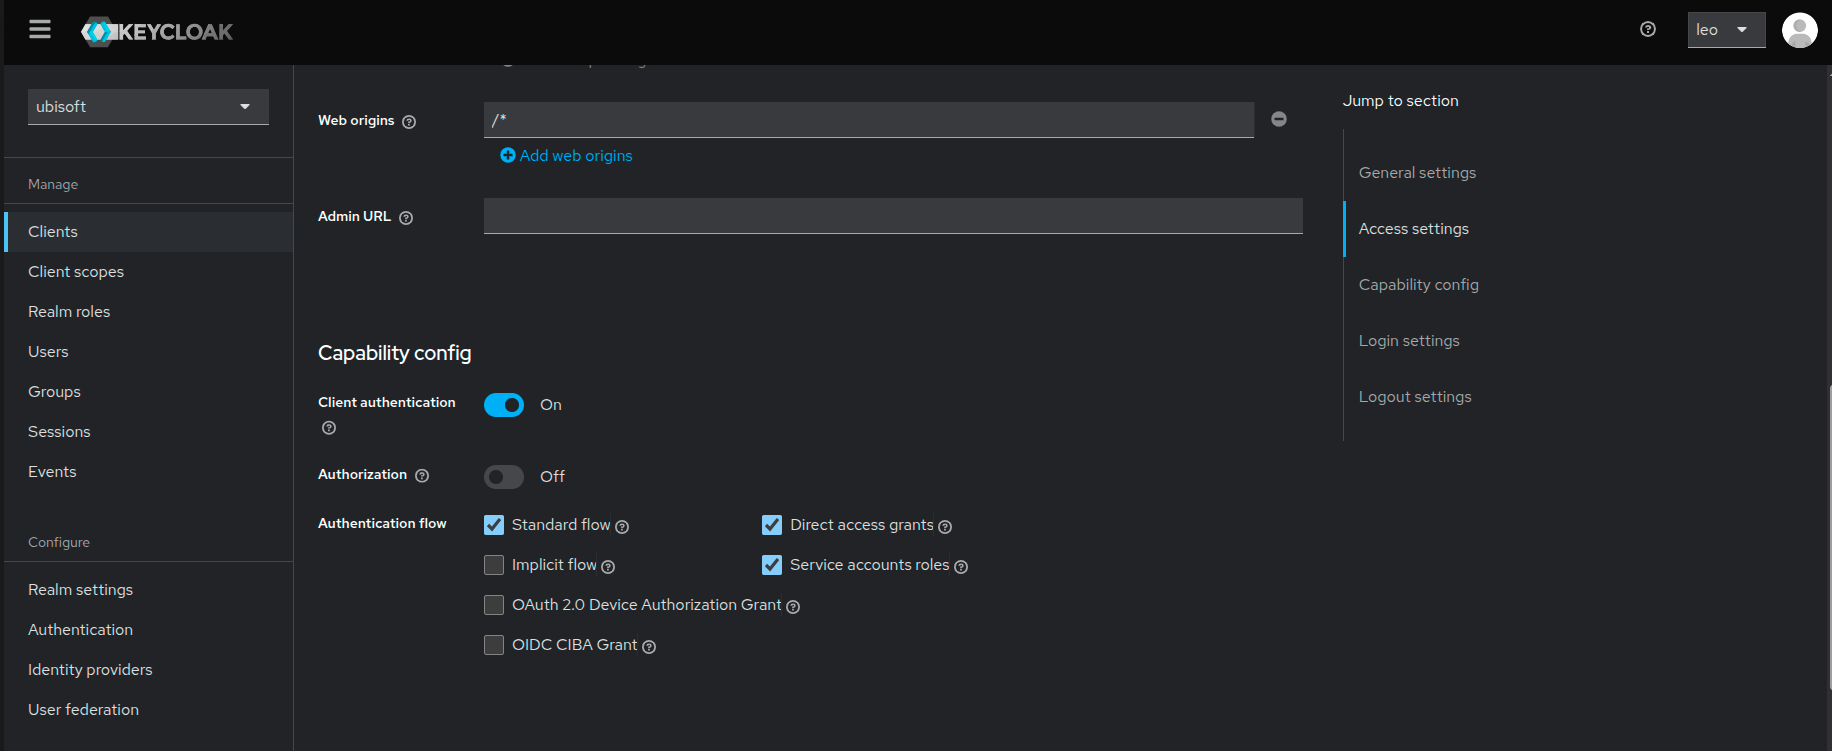
\includegraphics[width=1.0\linewidth]{Bilder/screenshot013}
		\caption{Beispielhafte Konfiguration von Authentication Flows in Keycloak: Hier ist bspw. die Client Authentication, Standard Flow, Service Accounts Roles und Direct Access Grant aktiviert.}
		\label{fig:screenshot013}
	\end{figure}
	Zudem unterscheidet Keycloak zwei zentrale Rollentypen:
	\begin{itemize}
		\item \textbf{\gls{realmrole}s:} Gültig innerhalb eines gesamten Realms und geeignet für übergreifende Rechte, z.\,B. \textit{\gls{realmadmin}} für alle Clients.
		\item \textbf{\gls{clientrole}a:} Spezifisch für einen einzelnen Client und ermöglichen eine feinere Zugriffskontrolle innerhalb der jeweiligen Anwendung, z.B. \textit{\gls{viewevents}}.
	\end{itemize}
	\textbf{\gls{serviceaccount} Roles:}\\
	Clients können sich in Keycloak auch selbst authentifizieren, ohne Benutzerinteraktion. Wird die \textit{Service Account}-Funktion aktiviert, erhält der Client ein eigenes Konto, das mit Rollen ausgestattet werden kann, um Berechtigungen auf bestimmte Ressourcen oder Operationen zu erhalten, beispielsweise für automatisierte Backend-Operationen.

	\subsection{Komponenten der Log-Erzeugung}
	Keycloak generiert Logs über verschiedene Frameworks und Komponenten. Eines dieser Frameworks ist das Logging-Framework von JBoss \footnote{\url{https://www.redhat.com/de/technologies/jboss-middleware/application-platform}, letzter Zugriff am 28.August.2025}, wobei moderne Versionen von Keycloak zusätzlich das \textit{\gls{quarkus}-Framework} nutzen.
	\\[0.5em]
	Frühere Versionen von Keycloak basierten auf dem \textbf{\gls{wildfly}}-Anwendungsserver\footnote{Mehr Infos unter: \url{https://www.wildfly.org/},letzter Zugriff am 28.August.2025}, der die \textbf{\gls{jbosslogging}}-Infrastruktur einsetzte. Ab Keycloak Version 17 wurde WildFly durch das \textbf{Quarkus}-Framework ersetzt, das weiterhin JBoss Logging unterstützt.
	\\[0.5em]
	JBoss Logging fungiert in Keycloak als zentrale Logging-API. Es abstrahiert verschiedene Logging-Backends (z.\,B. \texttt{\gls{log4j}} und \texttt{\gls{slf4j}}) und ermöglicht die strukturierte Ausgabe sicherheitsrelevanter Informationen. Entwickler müssen sich dabei nicht auf ein spezifisches Logging-Backend festlegen, sondern können über die einheitliche JBoss-API unterschiedliche Ausgabekanäle konfigurieren, wie Konsole, Datei oder \gls{syslog}.
	\\[0.5em]
	Ursprünglich wurden Logs für diese Arbeit über JBoss Logging direkt an ein Terminal ausgegeben. In späteren Versionen wurde entschieden, die Keycloak-API für die Log-Ausgabe zu verwenden. Detaillierte Informationen zur Nutzung der API werden in den folgenden Kapiteln behandelt.
	\\[0.5em]
	Generell hat ein Log in Quarkus folgenden Aufbau: 
	\texttt{[Datum, Zeit] [Log-Typ] [Java-Klasse] [Fehlermeldung]}.
	
	\begin{figure}[H]
		\centering
		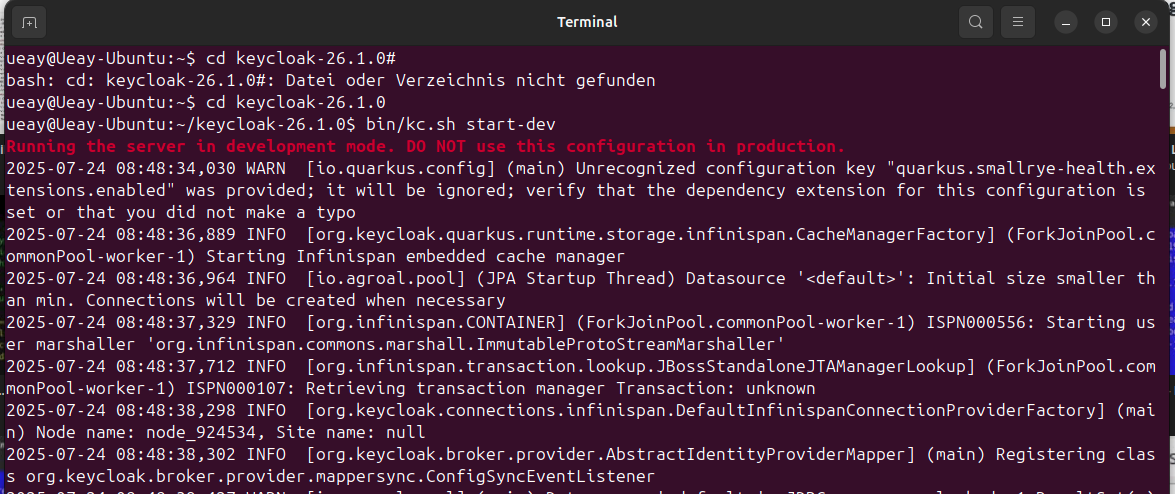
\includegraphics[width=1.1\linewidth]{Bilder/screenshot014}
		\caption{Log-Ausgaben aus einer Quarkus-basierten Keycloak-Instanz.}
		\label{fig:screenshot014}
	\end{figure}
	Insgesamt stellt die Kombination von JBoss Logging und Quarkus eine flexible und erweiterbare Logging-Lösung dar. In dieser Arbeit diente sie lediglich zu Beginn der Arbeitsphase dazu Orientierung zu gewinnen, wie die Keycloak-Logs aufgebaut sind und den ersten Ansatz (s. Kapitel 8) zu realisieren.
	
	\subsection{Log-Dateien in Keycloak}
	Logging bzw. Protokollierung ist ein essenzieller Bestandteil der Überwachung von IT-Systemen. Logs dienen im IT-Monitoring der Prävention und Detektion von Anomalien, sei es im Netzwerk, auf IoT-Geräten oder innerhalb von IAM-Softwarelösungen.
	\\[0.5em]
	Keycloak unterteilt Logs in folgende Kategorien:
	
	\begin{itemize}
		\item \gls{serverlogs}: Informationen zum Betriebsstatus, Fehler- und Debugging-Informationen
		\item \gls{eventlogs}: Benutzer- und Admin-Events
		\item \gls{auditlogs}: Nachvollziehbarkeit von Änderungen durch Administratoren.  Audit-Logs gelten als Unterkategorie der Event-Logs. 
		\item \gls{accesslogs}: Zugriffsversuche und HTTP-Statuscodes (HTTP Layer / Reverse Proxy)
		\item \gls{securitylogs}: Sicherheitsrelevante Ereignisse und Warnungen
		\item \gls{customlogs}: Erweiterungen und Plugins können eigene Logs erzeugen (\gls{spi})
	\end{itemize}
	Die Server-Logs werden vom Keycloak-Server erzeugt und über das Quarkus-Framework verarbeitet. Sie sind unter der Kategorie \textit{org.keycloak.services} zu finden.
	\\[0.5em]
	Event-Logs und Audit-Logs werden durch den \textit{EventListenerProvider} \footnote{\url{https://www.keycloak.org/docs-api/25.0.6/javadocs/org/keycloak/events/EventListenerProvider.html}, letzter Zugriff am 28.August.2025} in Keycloak erzeugt und unter der Kategorie \textit{org.keycloak.events} geführt. Access-Logs entstehen hingegen auf der Anwendungs- und Netzebene, meist außerhalb von Keycloak, und sind mit \textit{io.quarkus.http} gekennzeichnet.
	
	\subsection{Event-Logs und Audit-Logs}
	Für die Analyse in dieser Arbeit werden die Event-Logs und Audit-Logs betrachtet. Diese enthalten zentrale Informationen zum Benutzerverhalten.
	\\[0.5em]
	Nicht untersucht werden in dieser Arbeit Server-Logs und Access-Logs, da diese durch andere Komponenten in Keycloak erzeugt werden und nicht direkt das Benutzerverhalten widerspiegeln, da sie netzbasierte Logs sind- wobei zur sie Analyse von ungewöhnlicher, genutzter Geräte auch dazu dienen, Anomalien zu erkennen. Da diese Arbeit hauptsächlich Intrusionen und Insider-Attacken direkt durch ungewöhnliches Verhalten erkennen will und nicht durch Geräte, werden nur die beiden Event-Typen Event-Logs und Audit-Logs genutzt.
	Da keine SPI verwendet wird und nur eine einzelne Keycloak-Instanz untersucht wird, fallen Custom-Logs als Trainingsdaten weg.
	\\[0.5em]
	Keycloak unterscheidet zwei Arten von Event-Logs:
	\begin{itemize}
		\item Admin-Logs (Audit-Logs)
		\item User-Logs
	\end{itemize}
	Admin-Logs dokumentieren alle Admin-Operationen, während User-Logs ausschließlich Ereignisse regulärer Benutzer enthalten.
	
	\subsection{Aufbau der Event-Logs}
	Typische Features in den User-Event-Logs sind:
	\begin{itemize}
		\item \gls{timestamp}
		\item \gls{loglevel}
		\item \gls{logcategory}
		\item type
		\item ipAddress
		\item realmId
		\item clientId
		\item userId
	\end{itemize}
	Wichtige Informationen, wie z.\,B. der Standort des Benutzers, fehlen aus datenschutzrechtlichen Gründen. Dies kann die Erkennung von Anomalien erschweren, da ungewöhnliche Standorte (z.\,B. Pentagon) nicht identifiziert werden können. Timestamp hingegen ist ein zentrales Feature, das den Zeitpunkt der Log-Erstellung angibt und sich für Analysen über lange Zeit, wie etwa mit LSTM-Autoencoder-Hybridmodellen, eignet.
	\\[0.5em]
	Das Feature "category" beschreibt, aus welchem Modul das Log erzeugt wurde. Darüber hinaus sind die Ereignis-Typen ( "type" hier) relevant. 
	\\[0.5em]
	Beispielsweise bezeichnet LOGIN einen Event-Typ, der ausgelöst wird, wenn ein Benutzer sich anmeldet. Weitere Event-Typen sind bspw. \gls{refreshtoken}, bei dem ein Nutzer einen neuen Token erhält.
	\\[0.5em]
	Keycloak unterscheidet zudem verschiedene Log-Level, welche den Erfolg einer Operation anzeigen oder zusätzliche Informationen bereitstellen. Bekannte Log-Level sind z.\,B. INFO, FATAL oder ERROR \footnote{ \url{https://www.keycloak.org/server/logging}, letzter Zugriff am 28.August.2025}. Das Log-Level bestimmt, ob ein Eintrag der Fehlerbehebung, Warnung oder allgemeinen Information dient. Zudem kann man steuern, welche Logs ausgegeben werden, wenn man die  bestimmte Berechtigung (\textit{Maintainer}) dazu hat.
	
	\begin{figure}[H]
		\centering
		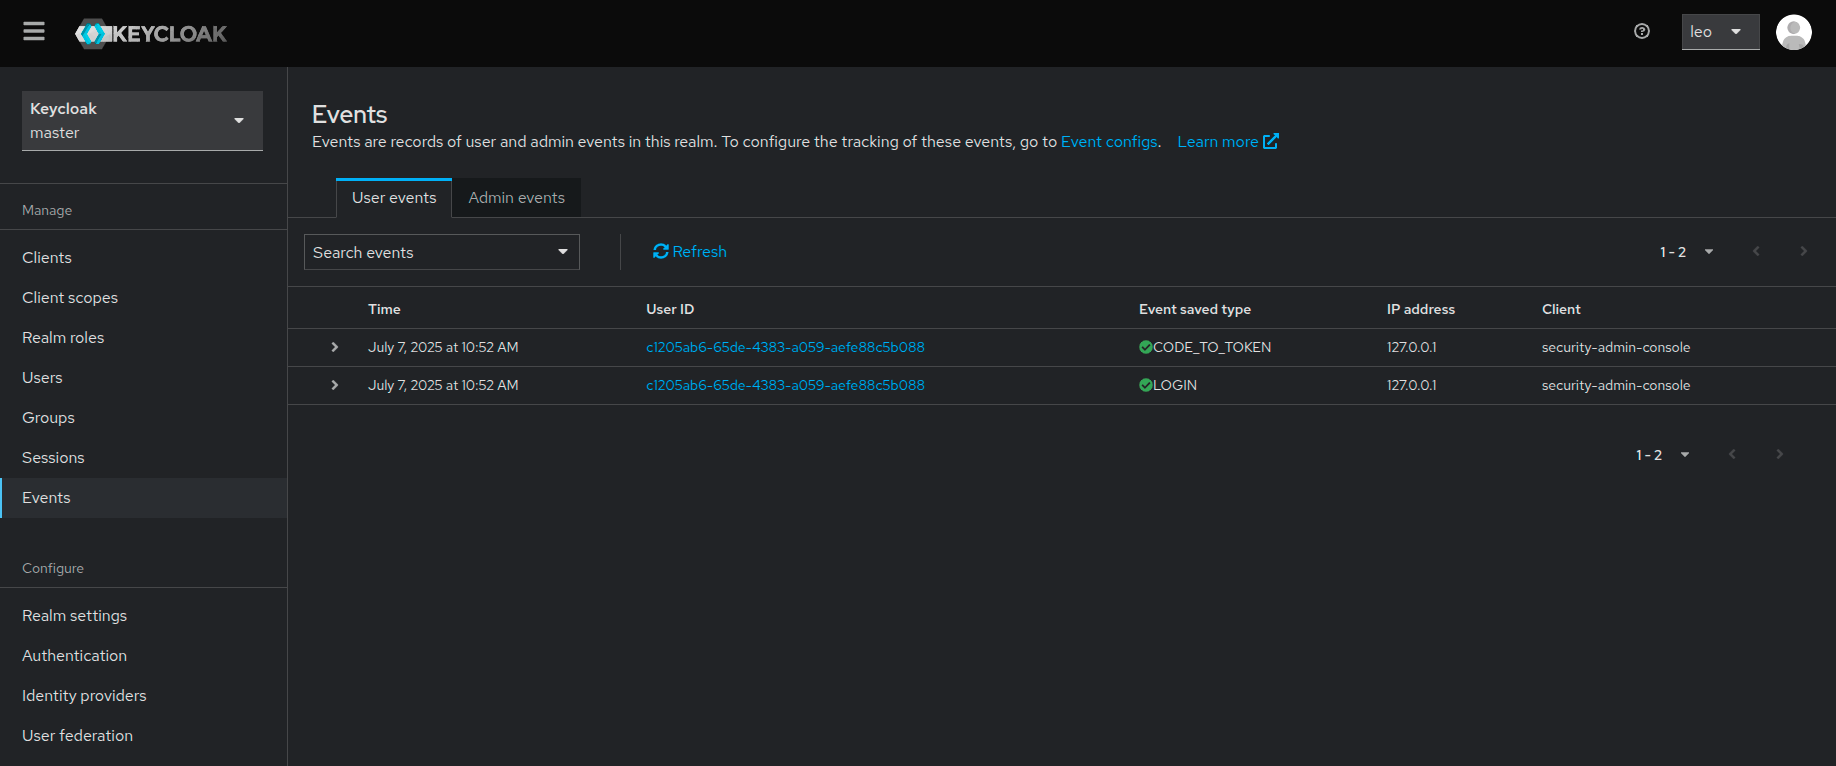
\includegraphics[width=1.0\linewidth]{Bilder/screenshot002}
		\caption{Hier kann man in Keycloak die User und Admin Events einsehen. Man erkennt hier in den User-Events schon ein paar Einträge mit dem entsprechenden Event-Typ}
		\label{fig:screenshot002}
	\end{figure}
	
	Je nach Event-Typ können zusätzliche Features aufgezeichnet werden. Beim LOGIN werden beispielsweise die Token-URL, Verbindungsart und das Authentifizierungsprotokoll protokolliert. Anhand Beispiele aus dem internen Unternehmen sind die häufigsten Event-Typen:
	
	\begin{itemize}
		\item LOGIN: Benutzer meldet sich erfolgreich über Keycloak an.
		\item \gls{codetotoken}: Wird erzeugt, sobald der Benutzer nach Authentifizierung einen Access Token erhält.
		\item \gls{clientlogin}: Log-Eintrag bei Anmeldung über einen Drittanbieter.
		\item \gls{loginerror}: Fehler beim Login über Keycloak.
		\item CODE TO TOKEN ERROR: Falsche Anmeldedaten, Server lehnt die Authentifizierung ab.
	\end{itemize}
	In den Admin-Logs sind zusätzliche Features enthalten, die in User-Logs nicht vorkommen, insbesondere das Feature \gls{operationtype}. Diese beschreiben typische CRUD-Operationen wie UPDATE, CREATE, DELETE und ACTION\footnote{ \url{https://github.com/keycloak/keycloak/blob/main/model/jpa/src/main/java/org/keycloak/events/jpa/JpaAdminEventQuery.java}, letzter Zugriff am 28.August.2025}.

	\section{Theoretischer Hintergrund der Modelle}
	\subsection{LSTM}
	Long Short-Term Memory (LSTM) ist ein spezieller Typ rekurrenter neuronaler Netzwerke (\gls{rnn}), welches entwickelt wurde, um Informationen über längere Zeiträume hinweg zu speichern und verarbeiten \cite{hochreiter1997long}. RNNs verarbeiten sequentielle Daten, bei denen die Reihenfolge der Eingaben eine zentrale Rolle spielt, und speichern frühere Informationen in einem sogenannten "\gls{hiddenstate}".
	\\[0.5em]
	Klassische RNNs stoßen bei langen Sequenzen auf das Problem des \gls{vanishing-gradient}, da der Gradient beim Zurückpropagieren über viele Zeitschritte sehr klein wird und frühere Informationen verloren gehen können. LSTMs umgehen dieses Problem durch eine spezielle Zellstruktur, die relevante Informationen über längere Zeiträume hinweg speichern kann \cite[S.19]{staudemeyer2019understanding}.
	\\[0.5em]
	LSTMs finden Anwendung in zahlreichen Bereichen, z.B. bei Vorhersagemodellen oder im Internet der Dinge (IoT) \cite{wei2022lstm}.
	\\[0.5em]
	Die Sequenzlänge und die Netzwerkgröße beeinflussen maßgeblich die Trainingsdynamik von rekurrenten neuronalen Netzen. Größere oder tiefere Netzwerke können komplexere Muster erfassen, erhöhen jedoch den Rechenaufwand und den Speicherbedarf. Insbesondere lange Sequenzen erschweren das Lernen, da die Gradienten während der Rückpropagation durch die Zeit entweder verschwinden oder explodieren können, was die Konvergenz des Trainings erschwert \cite{bengio1994learning}.
	\\[0.5em]
	Die Wahl der Sequenzlänge beeinflusst also nach Bengio den Lernerfolg des Modells. Sehr lange Sequenzen erhöhen die Komplexität des Trainings und erschweren die Konvergenz, während kürzere Sequenzen das Modell auf lokale Muster fokussieren und die Erkennung von Anomalien verbessern.
	\\[0.5em]
	Es gibt auch LSTM-Architekturen, welche flexibler und robuster mit der Sequenzlänge sind: "Hierarchisch-multiskalige" LSTM-Modelle lernen dynamisch, auf welchen Zeitskalen Informationen aktualisiert oder aggregiert werden sollten. Hierdurch können zeitliche Abhängigkeiten über lange Sequenzen effizienter modelliert werden, da das Modell gleichzeitig Abhängigkeiten auf mehreren Skalen berücksichtigt \cite{chung2017hierarchical}.
	\\[0.5em]
	LSTMs generalisieren Zählverhalten über deutlich längere Sequenzen oft nicht zuverlässig, selbst wenn sie es auf kürzeren Sequenzen scheinbar korrekt gelernt haben \cite{elnaggar2022counting}.
	\\[0.5em]
	Aufgrund der begrenzten Datenmenge und den genannten Nachteilen von langen Sequenzlängen liegt der Fokus auf kurzen Sequenzen. 
		
	\subsection{Autoencoder}
	Ein Autoencoder ist ein neuronales Netzwerk, das aus einer \gls{encoder}- und einer \gls{decoder}-Schicht besteht \cite[S.3]{michelucci2022introduction}. Der Encoder komprimiert die Eingabedaten in eine kompakte \gls{bottleneck}-Repräsentation, wodurch wesentliche Merkmale extrahiert und redundante Informationen reduziert werden. Der Decoder rekonstruiert anschließend die ursprünglichen Daten, wobei der \gls{rekonstruktionsfehler} – die Differenz zwischen Eingabe und Ausgabe – erzeugt wird.
	\\[0.5em]
	Signifikante Abweichungen von gelernten Mustern führen zu höheren Rekonstruktionsfehlern und markieren potenzielle Anomalien. Die Dimension des Bottlenecks spielt dabei eine entscheidende Rolle: Ein zu kleines Bottleneck kann relevante Informationen verlieren, während ein zu großes Bottleneck dem Netzwerk ermöglicht, die Daten ohne echte Verdichtung durchzuschleusen. Um die Extraktion vielfältiger Merkmale zu fördern, kann die Verlustfunktion modifiziert werden, sodass überlappende oder redundante Merkmale minimiert werden \cite{laakom2022reducing}.
	\\[0.5em]
	Erweiterte Autoencoder-Varianten umfassen beispielsweise den \gls{vae}, der probabilistische und generative Eigenschaften besitzt, sowie den \gls{denoising}-Autoencoder, der verrauschte Eingaben bereinigt. Mehrschichtige Autoencoder ermöglichen darüber hinaus die Extraktion komplexerer Merkmalsstrukturen. Studien zeigen, dass diese erweiterten Architekturen bei der Anomalieerkennung effektiver sind: So weisen Pantelidis et al. darauf hin, dass der VAE besser Anomalien erkennen kann als der normale Autoencoder \cite{Pantelidis2021}, Skaf et al. berichten eine bessere Leistung für den Denoising-AE \cite{Skaf2022}, und Wei et al. zeigen, dass mehrschichtige Autoencoder Anomalien besonders zuverlässig identifizieren können \cite{Wei2020}.

	\begin{figure}[H]
		\centering
		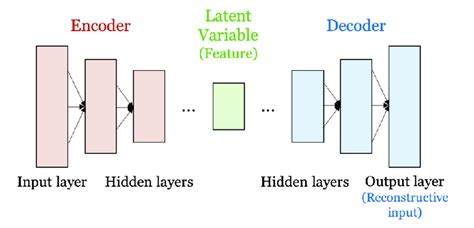
\includegraphics[width=0.7\linewidth]{Bilder/screenshot004}
		\caption{Visuelle Darstellung der Funktionsweise eines Autoencoders. Das Kästchen in der Mitte stellt den Bottleneck dar. [Online]. Quelle: \url{https://www.researchgate.net/figure/Structure-of-the-autoencoder\_fig1\_36507443}, letzter Zugriff am: 15.07.2025}
		\label{fig:screenshot004}
	\end{figure}
	Wie im Kapitel zum Forschungsstand diskutiert, lassen sich besonders Autoencoder effektiv mit LSTM-Netzwerken kombinieren, wenn es um sequenzielle oder zeitabhängige Daten geht. Ein LSTM-Autoencoder verwendet LSTM-Zellen im Encoder und Decoder, um komplexe zeitliche Muster zu erfassen und zu rekonstruieren. Diese Architektur ist insbesondere für die Anomalieerkennung in Zeitreihen geeignet, beispielsweise in der Überwachung von Maschinenzuständen, Finanzdaten oder der Netzwerksicherheit. Anomalien manifestieren sich häufig durch signifikant erhöhte Rekonstruktionsfehler, da zeitliche Muster nicht korrekt rekonstruiert werden können.
	
	\subsection{Isolation Forest}
	Isolation Forest ist ein unüberwachter Lernalgorithmus, der Daten durch Partitionierung trennt, indem er binäre Bäume erzeugt. Dabei werden die Daten so lange aufgeteilt, bis keine weitere Isolierung möglich ist. Dieses Vorgehen erlaubt es, Anomalien zu erkennen: Datenpunkte, die in wenigen Partitionierungsschritten isoliert werden, gelten als potenzielle Anomalien. Datenpunkte, die ähnliche Merkmalswerte aufweisen, werden dagegen nicht stark isoliert. Je stärker sich ein Datenpunkt anhand seiner Merkmale isolieren lässt, desto wahrscheinlicher ist es, dass er keiner üblichen Menge zugeordnet werden kann \cite[S. 2]{liu2008isolation}. Isolation Forest eignet sich zudem für hochdimensionale Daten \cite[S. 10]{liu2008isolation}.
	\\[0.5em]
	\begin{figure}[H]
		\centering
		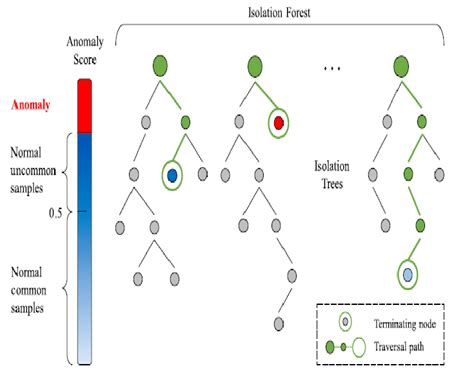
\includegraphics[width=0.9\linewidth]{Bilder/screenshot005}
		\caption{Visuelle Darstellung der Funktionsweise des Isolation Forest [Online]. Quelle: \url{https://www.researchgate.net/figure/Anomaly-Detection-using-Isolation-Forest-18\_fig3\_350551253}, letzter Zugriff am: 15.07.2025}
		\label{fig:screenshot005}
	\end{figure}
	Ein \gls{isolationtree} besteht aus inneren Knoten und Blattknoten. Jeder innere Knoten enthält eine Testregel, die die Datenpunkte in zwei Gruppen aufteilt. Die Testregel basiert auf der Auswahl eines Merkmals \(q\) und eines Schwellenwerts \(p\): Datenpunkte mit einem Wert für \(q\) kleiner als \(p\) gelangen in den linken Kindknoten, alle anderen in den rechten.
	\\[0.5em]
	Zum Aufbau eines solchen Baums wird eine Stichprobe der Datenpunkte rekursiv aufgeteilt, wobei Merkmal und Split-Wert zufällig gewählt werden. Dieser Prozess wird so lange wiederholt, bis  
	\begin{itemize}
		\item die maximale Baumhöhe erreicht ist,
		\item nur noch ein Datenpunkt im Teilbaum übrig ist, oder
		\item alle Datenpunkte im aktuellen Teilbaum identisch sind \cite[S.3]{liu2008isolation}.
	\end{itemize}
	Das Ergebnis ist ein vollständiger binärer Baum, bei dem jeder Datenpunkt in einem Blattknoten isoliert wird.
	\\[0.5em]
	Wenn alle Datenpunkte unterschiedlich sind, gilt:  
	\begin{itemize}
		\item Die Anzahl der Blattknoten entspricht der Anzahl der Datenpunkte \(n\).  
		\item Die Anzahl der inneren Knoten beträgt \(n-1\).  
		\item Insgesamt besitzt der Baum \(2n-1\) Knoten.  
		\item Der Speicherbedarf wächst somit linear mit der Anzahl der Datenpunkte.
	\end{itemize}
	Isolation Forest unterteilt die Datenpunkte zufällig, was die Nachvollziehbarkeit der Partitionen einschränkt, jedoch die Effizienz des Algorithmus steigert.
	
	\subsection{One-Class SVM}
	OCSVM ist ein unüberwachter Algorithmus, der Anomalien erkennt, indem er eine Trennlinie (oder Grenzfläche) zwischen normalen Datenpunkten und potenziellen Ausreißern in einem hochdimensionalen Raum lernt, wobei die Flexibilität der Kernelmethoden es erlaubt, auch komplexe Grenzen zu modellieren \cite{Yang2021}.
	\\[0.5em]
	Zur Modellierung dieser Support-Region wird eine Funktion \(f(x)\) gelernt, die auf den meisten Trainingsdaten positive Werte annimmt und auf Punkten außerhalb der Verteilung negative Werte. Durch den Einsatz von Kernelfunktionen kann die OCSVM auch komplexe, nichtlineare Grenzen um die Datenverteilung modellieren. Auf diese Weise identifiziert das Modell effektiv Ausreißer, die sich deutlich von den normalen Mustern unterscheiden \cite[S.6]{Scholkopf2001}.
	\\[0.5em]
	Viele Angriffe lassen sich durch die Analyse von System-Logdaten erkennen. Ein Ansatz auf Basis der OCSVM wurde beispielsweise mit abstrahierten Benutzeraudit-Logs aus dem DARPA-Datensatz von 1999 trainiert \cite{li2003improving}. Durch die Abbildung der Daten in einen höherdimensionalen Raum können auch nichtlinear trennbare Daten effektiv separiert werden, wodurch die OCSVM für die Anomalieerkennung geeignet ist.
	\\[0.5em]
	\begin{figure}[H]
		\centering
		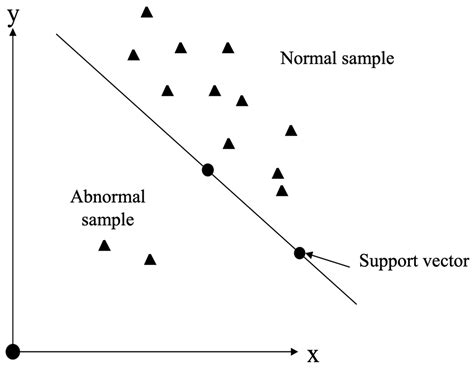
\includegraphics[width=0.7\linewidth]{Bilder/screenshot006}
		\caption{Visuelle Darstellung der OCSVM [Online]. Quelle: \url{https://www.mdpi.com/2076-3417/13/3/1734}, letzter Zugriff am: 15.07.2025}
		\label{fig:screenshot006}
	\end{figure}
	Ein zentrales Problem der OCSVM besteht darin, dass der Ursprung im \gls{featurespace} als Referenzpunkt für Anomalien dient, was in der Praxis nicht immer zutrifft \cite{bounsiar2014oneclass}. Die Autoren erklären, dass die Trennung der Zielklasse vom Ursprung – also von den potenziellen Ausreißern – häufig missverstanden wird. Sie schlagen eine geometrische Interpretation vor, bei der die Zielklasse vom übrigen Raum getrennt wird, insbesondere wenn ein Gauß-Kernel verwendet wird. Da diese Arbeit jedoch Klassen von Scikit verwendet, wird stattdessen der RBF-Kernel verwendet. Die Nachteile von OCSVM wird wie bei IF und DBSCAN durch Parametrisierung ausgeglichen.
	
	\subsection{DBSCAN}
	DBSCAN (Density-Based Spatial Clustering of Applications with Noise) ist ein dichtebasiertes Clusteringverfahren, das Datenpunkte anhand ihrer lokalen Dichte gruppiert \cite{ester1996dbscan}.
	\\[0.5em]
	Die Dichte wird durch die Anzahl der Nachbarpunkte innerhalb eines definierten Radius (\( \text{Eps} \)) bestimmt. Ein Punkt gilt als Kernpunkt, wenn sich mindestens eine vorgegebene Mindestanzahl von Punkten (\( \text{MinPts} \)) innerhalb dieses Radius befindet. Die Wahl dieser Parameter ist entscheidend für die Qualität der Clusterbildung.
	\\[0.5em]
	\begin{figure}[H]
		\centering
		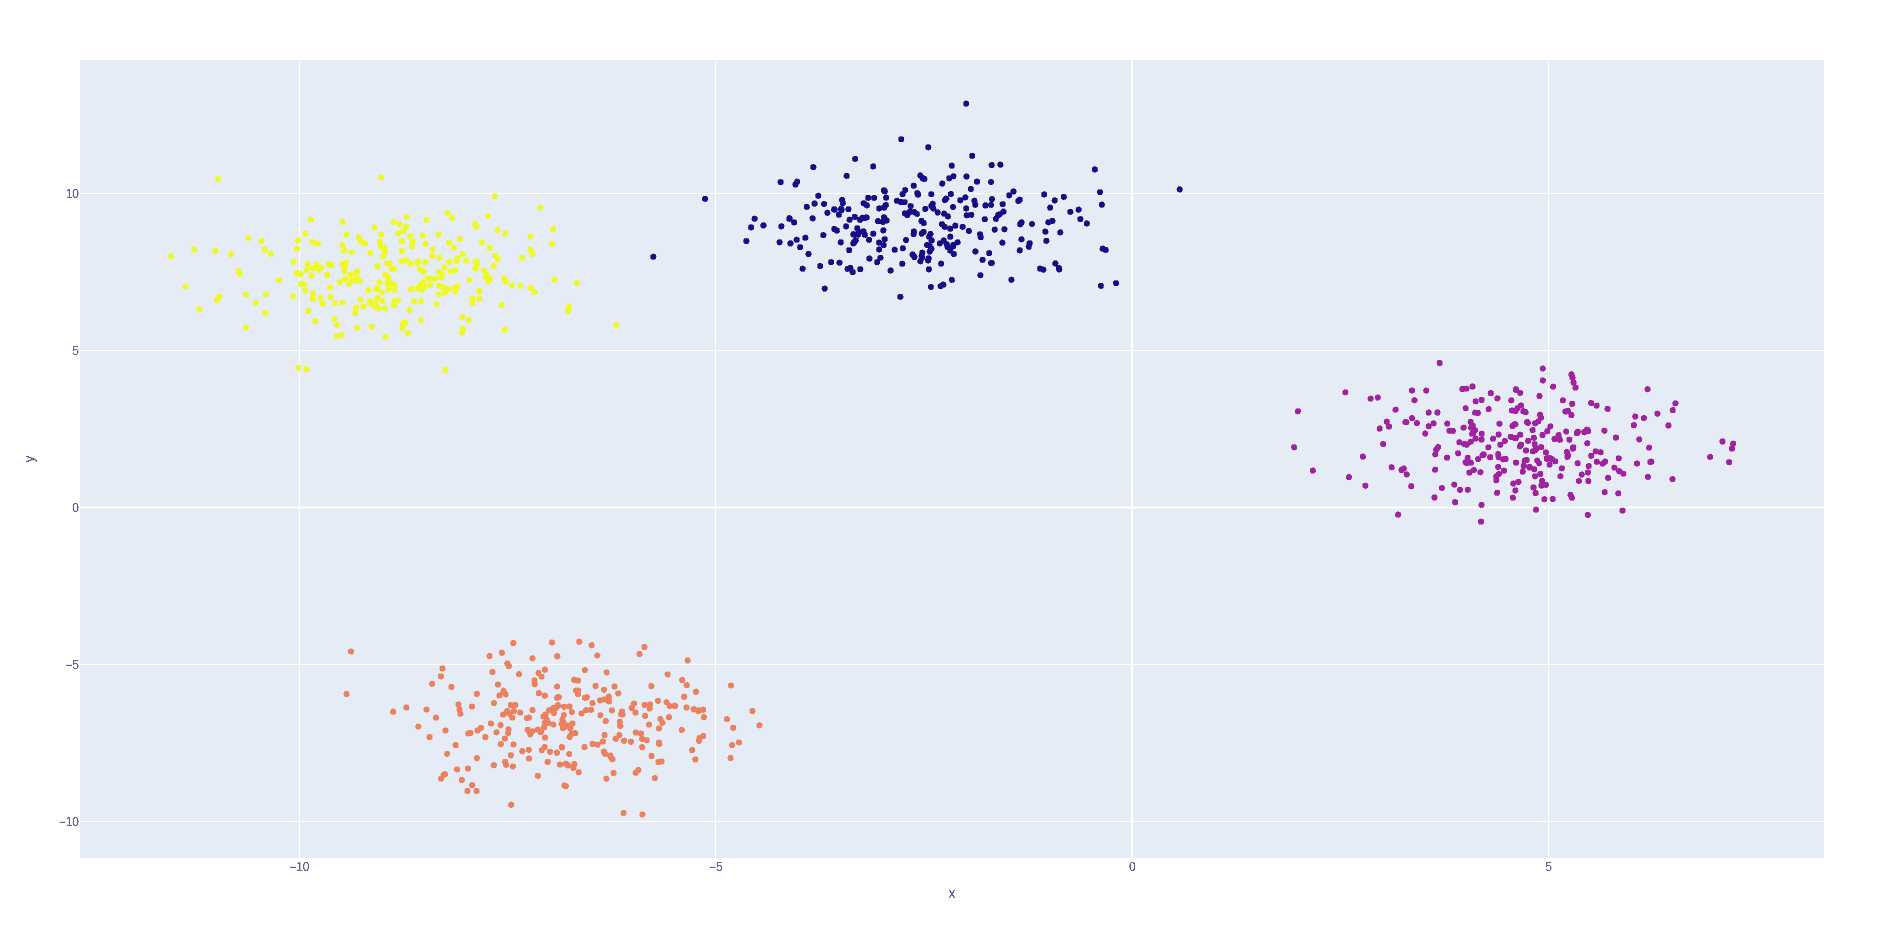
\includegraphics[width=0.9\linewidth]{Bilder/screenshot015}
		\caption{Beispielhafte Darstellung von DBSCAN-Clustern. Quelle: \url{https://www.baeldung.com/wp-content/uploads/sites/4/2023/04/clusters.png}, letzter Zugriff am: 15.07.2025}
		\label{fig:screenshot015}
	\end{figure}
	Der Algorithmus arbeitet wie folgt:  
	\begin{enumerate}
		\item Ein unbesuchter Punkt \(p\) wird ausgewählt.
		\item Alle Punkte, die sich innerhalb des Radius \(\text{Eps}\) um \(p\) befinden, werden bestimmt.
		\item Bildet \(p\) zusammen mit seinen Nachbarn einen Kernpunkt (d.h. die Anzahl der Nachbarn \(\geq \text{MinPts}\)), wird ein neues Cluster gebildet. Alle direkt dichten Nachbarn werden in dasselbe Cluster aufgenommen.
		\item Jeder Punkt, der keinem Cluster zugeordnet werden kann, wird als Rauschpunkt (\textit{Noise}) markiert.
		\item Der Vorgang wird wiederholt, bis alle Punkte besucht wurden.
	\end{enumerate}
	Eine hohe Anzahl von Rauschpunkten kann darauf hinweisen, dass die Parameterwahl oder die Klassifikation nicht optimal ist \cite{ester1996dbscan}.
	
	\subsection{Weitere Algorithmen für zukünftige Studien }
	Als Alternative zu DBSCAN wurde auch das hierarchische Verfahren \gls{hdbscan} (Hierarchical Density-Based Spatial Clustering of Applications with Noise) in Betracht gezogen. HDBSCAN ist in vielerlei Hinsicht robuster als DBSCAN, insbesondere bei der Identifikation von Clustern in hochdimensionalen oder verrauschten Daten \cite{campello2015hierarchical}. Ein Vorteil von HDBSCAN besteht darin, dass keine globale Dichte-Schwelle erforderlich ist und sich das Verfahren besser an lokale Datenstrukturen anpasst. Für zukünftige Arbeiten wäre eine Untersuchung von HDBSCAN in Kombination mit LSTM-Autoencodern denkbar.
	\\[0.5em]
	Darüber hinaus wurden weitere Anomalieerkennungsverfahren evaluiert, darunter \gls{kmeans} und \gls{lof} (Local Outlier Factor). K-Means wird in der Studie von Vinces et Al. als besonders effektiv eingeschätzt \cite{vinces2025comparative}. LOF erkennt Ausreißer, indem die lokale Dichte eines Datenpunkts mit der seiner Nachbarn verglichen wird; Punkte mit stark abweichender Dichte werden als potenzielle Anomalien markiert. Die Wirksamkeit von LOF zur Anomalieerkennung wurde von Breunig nachgewiesen \cite{breunig2000lof}.
	\\[0.5em]
	Beide Verfahren eignen sich grundsätzlich für die Anomalieerkennung. Budiarto et Al. zeigen jedoch, dass OCSVM mehr Anomalien erkennen kann als die beiden Verfahren \cite{budiarto2025unsupervised}. Zudem leidet LOF unter dem „Fluch der Dimensionalität“, da Dichte-Schätzungen im euklidischen Raum (z.B. k-Nächste-Nachbarn-Distanzen) in hochdimensionalen Räumen an Aussagekraft verlieren \cite[S.366]{zimek2012survey}. 
	\\[0.5em]
	DBSCAN, OCSVM und Isolation Forest wurden trotz ähnlicher Einschränkungen ausgewählt, um eine möglichst hohe Varianz in der Methodenauswahl zu gewährleisten. Algorithmen mit stark ähnlicher Funktionsweise, wie K-Means (Clustering-Ansatz ähnlich DBSCAN) oder LOF (Parallelen zum Isolation Forest), könnten in weiteren Studien noch genauer untersucht werden. Ein weiterer Entscheidungsgrund war die Skalierbarkeit: K-Means ohne Optimierungsmechanismen bspw. stößt bei großen Datensätzen an Grenzen \cite{mussabayev2023kmeans}.
	\\[0.5em]
	Auch das LOF-Verfahren kann bei großen Datenmengen ohne Performance-Optimierung hohe Rechenzeiten verursachen; entsprechende Ansätze zur Verbesserung der Laufzeit, etwa durch Block-Größe-Optimierung, werden derzeit erforscht \cite{springerlof2023}.
	\\[0.5em]
	Wie im Abschnitt zu Autoencodern bereits erläutert, existieren diverse Varianten, die potenziell eine präzisere Anomalieerkennung ermöglichen. In der vorliegenden Arbeit wird jedoch auf eine Evaluierung dieser Alternativen verzichtet, da der Fokus auf dem LSTM-Autoencoder in Kombination mit anderen Algorithmen liegt. Ausschlaggebend hierfür ist insbesondere die vergleichsweise einfache Implementierung des LSTM-Autoencoders sowie die Verfügbarkeit detaillierter Anleitungen zu dessen Aufbau und Training.

	\section{Implementierung}
	\subsection{Hybridmodelle mit LSTM-AE}
	Die Modelle wurden nach einer einheitlichen Architektur implementiert:. 
	
	\begin{table}[H]
		\centering
		\begin{tabular}{ll}
			\toprule
			\textbf{Parameter} & \textbf{Wert} \\
			\midrule
			\gls{batchsize} & 32 \\
			%\gls{dropoutrate} & 0.1
			encoder\_layers & [128, 64] \\
			decoder\_layers & [64, 128] \\
			\gls{learningrate} & 0.001 \\
			epochs & 50 \\
			\bottomrule
		\end{tabular}
		\caption{Ausgewählte Parameter der Modellkonfiguration}
		\label{tab:model_params}
	\end{table}
	
	Die Encoder- und Decoder-Architektur umfasst jeweils zwei Schichten mit den Dimensionen 128 und 64. Diese Konfiguration wurde gewählt, um eine ausreichende Komprimierung der zeitlichen Muster zu ermöglichen, ohne dass wesentliche Informationen verloren gehen. Eine geringere Breite würde die Informationsrepräsentation einschränken, während eine größere Tiefe zu Überanpassung führen könnte. Diese Parameterauswahl orientiert sich an Toor et al. \cite{Toor2022}, welche in LSTM-basierten Architekturen erfolgreich eingesetzt wurde.  
	\\[0.5em]
	Die Lernrate von 0.001 hat sich laut Santos et Al. als stabil erwiesen und bietet Vorteile gegenüber kleineren Lernraten wie 0.0001 \cite{Santoso2022}. Die Batch-Size von 32 wurde gewählt, da kleine Batches laut Masters und Luschi \cite{masters2018revisiting} die stabilste Trainingsdynamik erzielen.
	\\[0.5em]
	%	Zur Regularisierung wird eine Dropout-Rate von 0.1 verwendet. Während des Trainings werden somit zufällig einzelne Neuronen deaktiviert, um Overfitting zu reduzieren. Die geringe Dropout-Rate sorgt dafür, dass die Ergebnisse reproduzierbar bleiben, gleichzeitig aber die Robustheit der Modelle gegenüber neuen Daten verbessert wird \cite{Salehin2023}.  
	Zudem wird \textit{EarlyStopping}\footnote{\url{https://de.python-3.com/?p=45278}, letzter Zugriff am 28.August.2025}
	eingesetzt. Diese Technik verhindert Overfitting, indem das Training automatisch abgebrochen wird, sobald die Validierungsleistung über eine definierte Anzahl von Epochen (Patience) keine Verbesserung zeigt. Obwohl die maximale Epochenzahl auf 50 gesetzt ist, wird diese nicht zwingend erreicht; die tatsächlich trainierten Epochen variieren je nach Modell. Dabei wurde Patience auf 2 festgelegt. Nach Hussein et Al. wurde erkannt, dass eine Patience von 2 bei 20 Epochen ausreichend ist für einen geringen Validierungsverlust \cite{Hussein2024EarlyStopping}. Auch wenn die Patience von 5 die höchste Accuracy erzielte- waren diese Unterschiede sehr minimal. Man geht davon aus, dass dementsprechend eine Patience von 2 ausreichen. Da die Ressourcen dieser Arbeit (darunter auch Zeit) zudem begrenzt sind, entschied man sich darauf die Patience auf diese Anzahl zu setzen.
	\\[0.5em]
	Die Daten werden zunächst in numerische Form überführt, falls sie noch nicht numerisch sind. \gls{nan}- oder unklare Werte werden bewusst nicht bereinigt, sondern als eigene Kategorie behandelt, um potenzielle Anomalien nicht zu entfernen. Diese Transformation erfolgt mittels LabelEncoder\footnote{\url{https://scikit-learn.org/stable/modules/generated/sklearn.preprocessing.LabelEncoder.html}, letzter Zugriff am 28.August.2025}. Anschließend werden die Daten mit dem StandardScaler normalisiert\footnote{\url{https://scikit-learn.org/stable/modules/generated/sklearn.preprocessing.StandardScaler.html}, letzter Zugriff am 28.August.2025}. 
	\\[0.5em]
	Obwohl die Mehrheit der Merkmale kategorial war, wurde auf ein One-Hot-Encoding \footnote{\url{https://scikit-learn.org/stable/modules/generated/sklearn.preprocessing.OneHotEncoder.html}, letzter Zugriff am 28.August.2025} bewusst verzichtet. Stattdessen kam ein Label-Encoding zum Einsatz, um die Eingabedimension kompakt zu halten und eine effiziente Sequenzverarbeitung im LSTM zu ermöglichen. Ein One-Hot-Encoding hätte bei den zahlreichen Kategorien zu einer stark erhöhten Vektordimension geführt und damit sowohl Trainingszeit als auch Speicherbedarf deutlich gesteigert. Für die vorliegende Aufgabe der Anomalieerkennung ist eine kontinuierliche numerische Repräsentation ausreichend, da das Ziel nicht die Klassifikation einzelner Kategorien, sondern die Erkennung von Abweichungen in den Sequenzmustern ist. 
	
	\begin{figure}[H]
		\centering
		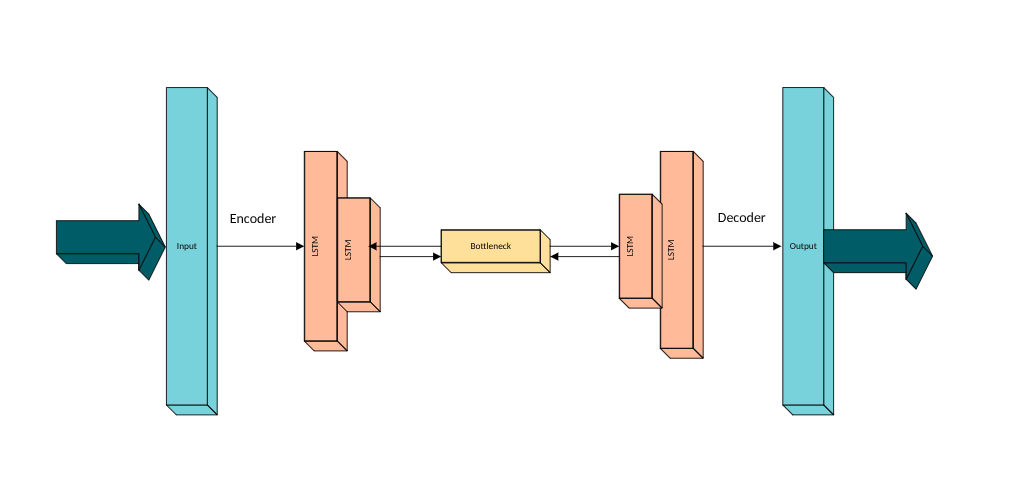
\includegraphics[width=0.9\linewidth]{Bilder/screenshot-lstm}
		\caption{Gesamtarchitektur des LSTM-Autoencoders}
		\label{fig:screenshot-lstm}
	\end{figure}
	Die Rekonstruktionsfehler des LSTM-AE werden anschließend von den Anomalieerkennungs-Algorithmen verarbeitet, wie auch in Malhotra et al. \cite{malhotra2016lstm} gezeigt wird. Diese modulare Struktur erlaubt ein separates Training, Testen und Evaluieren der einzelnen Modelle. Die Implementierung erfolgt in einem \gls{jupyternotebook}.
	
	\paragraph{Encoder-Decoder Struktur und Bidirektionales LSTM}  
	Die Architektur folgt dem Prinzip eines Encoder-Decoder-Systems, bei dem der Encoder die wesentlichen Merkmale der Eingabesequenzen in einem kompakten latenten Raum repräsentiert. Dieser latente Raum fasst die zeitlichen Muster zusammen und ermöglicht eine effiziente Datenrepräsentation. Das bidirektionale LSTM im Encoder erfasst dabei sowohl Informationen aus der Vergangenheit als auch aus der Zukunft der Sequenz. Dies ist insbesondere bei der Erkennung von Angriffs- oder Anomalieszenarien von Vorteil, da potenziell verdächtige Ereignisse oft nur im Kontext benachbarter Zeitpunkte eindeutig identifiziert werden können. Der Decoder nutzt die latente Repräsentation, um die ursprüngliche Sequenz zu rekonstruieren, wodurch eine präzise Nachbildung der Eingabedaten ermöglicht wird. Nach Acharya et Al. eignet sich ein bidirektionales LSTM optimal zur Anomalieerkennung \cite{acharya2023bidirectional}.

	\paragraph{Verlustfunktion und Optimierung}  
	Zur Bewertung der Modellgüte wird die mittlere quadratische Abweichung ( \gls{mse} \footnote{Definition des MSE: https://scikit-learn.org/stable/modules/generated/sklearn.metrics.mean\_squared\_error.html}) herangezogen, welche die Differenz zwischen Eingabe- und Ausgabesequenzen quantifiziert. MSE eignet sich zur Messung der Rekonstruktionsqualität bei kontinuierlichen Werten, da größere Fehler durch die Quadratisierung stärker gewichtet werden, was eine präzise Anpassung des Modells erzwingt. 
	\\[0.5em]
	Die Optimierung erfolgt mittels des \gls{adam}-Optimierers \footnote{Definition des Adam-Optimierers: \url{https://docs.pytorch.org/docs/stable/generated/torch.optim.Adam.html}, letzter Zugriff am 18. August 2025}, welcher durch Lernraten für jeden Parameter besticht und somit eine schnelle und stabile Konvergenz auch bei komplexen Modellen gewährleistet. Die Lernrate stellt dabei einen wesentlichen Hyperparameter dar, der das Tempo der Gewichtsaktualisierungen steuert und einen Balanceakt zwischen schnellem Lernen und stabiler Anpassung darstellt. 
	\\[0.5em]
	Gudla et Al. zeigen bspw., dass der Adam-optimierer sich mit einer Lernrate von 0.001 optimal für LSTM-Netzwerke eignet, um bspw. DDoS-Angriffe zu erkennen \cite{Gudla2023}.
	
	\paragraph{Berechnung des Rekonstruktionsfehlers}
	Die Idee, dass sich Mean Square Error den Rekonstruktionsfehler ist inspiriert von einer Studie von Torabi et Al. \cite[S. 5]{torabi2023practical}. Die allgemeine Formel zur Berechnung des Fehlers lautet wie folgt:
	
	\[
	\text{Reconstruction Error} = \frac{1}{T \cdot F} \sum_{t=1}^{T} \sum_{f=1}^{F} \left( x_{t,f} - \hat{x}_{t,f} \right)^2
	\]
	Im Grunde genommen wird hier jeder Fehler als Zeitpunkt dargestellt. Jeder Zeitpunkt (I) und jedes Feature F stellt hier eine Abhängigkeit dar. Alle rekonstruierbaren Werte werden von den nicht-rekonstruierbaren über jedes Logs hinweg berechnet – und anschließend wird der Durchschnitt berechnet. Dies ist dann der gesamte Rekonstruktionsfehler.
	
	\paragraph{Ermittlung des Schwellenwertes}
	Die Frage, ab welchem Punkt ein Modell eine Anomalie erkennen sollte, ist entscheidend für die Güte der Detektion: Soll bereits eine geringe Abweichung eines Features als Anomalie gelten, oder erst größere Diskrepanzen? Jablonski et al. \cite{jablonski2023automatic} schlagen hierfür einen algorithmischen Ansatz vor: Zunächst werden alle Rekonstruktionsfehler aus den Daten extrahiert. Anschließend wird der optimale Schwellenwert algorithmisch anhand der größten Lücke im sortierten Fehlervektor bestimmt – also zwischen den beiden Werten, die im Fehlervektor am weitesten auseinanderliegen. 
	\\[0.5em]
	Die Arbeit von Jablonski et Al. inspirierte dazu, einen eigenen Ansatz zu entwickeln: Zunächst werden alle Rekonstruktionsfehler aus den Daten extrahiert und sortiert. Der optimale Schwellenwert wird dann als die Mitte zwischen den beiden Werten mit dem größten Abstand im sortierten Fehlervektor definiert.
	\\[0.5em]
	In dieser Arbeit wurde dieser erfundene Ansatz jedoch verworfen, da er zu geringeren Precision- und Recall-Werten in allen Hybridmodellen führt. Vermutlich liegt dies daran, dass Anomalien im Verhältnis zur Gesamtanzahl normaler Logs sehr selten auftreten. Für eine zuverlässige Anomalieerkennung in Zeitreihen ist es daher notwendig, die Rohwerte der Anomalie-Scores (also die vom Modell berechneten Rekonstruktionsfehler) in binäre Entscheidungen zu überführen. Hierzu wird ein Schwellenwert festgelegt: Werte oberhalb des Schwellenwerts werden als Anomalien klassifiziert, Werte darunter als normal.
	\\[0.5em]
	Die Wahl des Schwellenwerts beeinflusst direkt das Verhältnis zwischen Precision (Anteil korrekt erkannter Anomalien unter allen als anomal klassifizierten Punkten) und Recall (Anteil erkannter Anomalien unter allen tatsächlichen Anomalien). Um dieses Verhältnis optimal zu berücksichtigen, wird der F1-Score als kombinierte Kennzahl verwendet. Der Schwellenwert wird so gewählt, dass der F1-Score maximiert wird. Es ist auch in der Literatur als verlässliche Methode zur Bestimmung von Schwellenwerten etabliert \cite{wilkinghoff2024f1ev}. Dabei gehen Wilkinghof et Al. noch ein wenig weiter und schlagen einen neueren Ansatz vor, nämlich, den "F1-EV Score" zu verwenden. Man entschied sich jedoch nur dazu den F1-Score zu optimieren, weil dies praktischer umzusetzen war in dieser Arbeit.
	
	\subsubsection{Implementierung: Isolation Forest und OCSVM}
	Anstatt die standardmäßige Vorhersage (-1 = anomal, 1 = normal) direkt zu verwenden, werden die Rohscores \footnote{Viele Modelle geben keine direkten Wahrscheinlichkeiten, sondern numerische Scores aus, die anzeigen, wie stark das Modell zu einer Klasse tendiert. Dies ist dann ein Rohscore} des Modells genutzt, um mittels einer F1-basierten Schwellenwert-Optimierung \cite{wilkinghoff2024f1ev} eine binäre Klassifikation zu erzeugen. Für jeden Testpunkt wird dabei ein optimaler Schwellenwert bestimmt, der die F1-Metrik maximiert. Alle Punkte mit Scores oberhalb dieses Schwellenwerts werden als Anomalien (1) klassifiziert, alle anderen als normal (0). Diese Vorgehensweise ist besonders sinnvoll, da Anomalien in Zeitreihendaten häufig selten auftreten und eine Balance zwischen Precision und Recall entscheidend ist.
	\\[0.5em]
	Da die Daten sequenzbasiert aufgebaut sind, wird jedes Fenster der Sequenz bewertet: Wenn innerhalb des Fensters mindestens ein Punkt anomal ist, erhält das Fenster das Label 1, sonst 0. Dadurch werden die binären Vorhersagen konsistent mit den Testlabels verglichen.
	\\[0.5em]
	Dieser Ansatz erfolgt für IF und OCSVM. 
	\\[0.5em]
	Die Parameter des IF werden folgendermaßen gesetzt:
	\begin{itemize}
		\item contamination= 0.0008
		\item random\_state= 42
		\item max\_samples= auto
	\end{itemize}
	
	Die Parameter des OCSVM werden folgendermaßen gesetzt:
	\begin{itemize}
		\item contamination= nu
		\item random\_state= 42
		\item kernel= rbf
		\item gamma= scale
	\end{itemize}
	
	Die Setzung von "contamination" und "nu" beruht auf den erwarteten Anomalien (wird in den Kapiteln bzgl. der Ansätze genauer erläutert). Der Parameter max\_samples wird auf Auto gesetzt, damit IF flexibel auf größere Datensätze reagiert. Der Parameter "random\_state" beleibt dem Standardwert 42. Bei OCSVM bleibt der Standardkernel auf "rbf" gesetzt für nicht-lineare Verarbeitung, sowie der Standardwert "scale" bei "gamma".
	
	\subsubsection{Implementierung: DBSCAN}
	Das DBSCAN-Modell wird direkt auf die skalierten Rekonstruktionsfehler der Testdaten angewendet. Dabei wird der Parameter \texttt{eps} automatisch über ein Raster von 0.01 bis 1.0 angepasst, sodass die Anzahl der als Anomalien klassifizierten Punkte ungefähr der erwarteten Anzahl an Anomalien entspricht. \texttt{min\_samples} wird auf 3 gesetzt, und die Distanzmetrik ist \texttt{euclidean}.  
	\\[0.5em]
	Die Methode \texttt{fit\_predict() \footnote{Detaillierte Dokumentation: \url{https://scikit-learn.org/stable/modules/generated/sklearn.cluster.DBSCAN.html}}} liefert für jeden Punkt entweder eine Clusterzuweisung (0, 1, …) oder -1. Punkte mit der Kennzeichnung -1 werden als Anomalien interpretiert.  
	\\[0.5em]
	Auf Basis der Vorhersagen werden verschiedene Evaluationsmetriken berechnet, darunter Precision, Recall, F1-Score, ROC-AUC, PR-AUC, Accuracy, Matthews-Korrelationskoeffizient (MCC) und Balanced Accuracy, um die Leistungsfähigkeit des Modells zu beurteilen.
	

	\subsection{Alternative Architekturen}
	Es ist ebenfalls möglich, zunächst eines der Algorithmen zu trainieren und anschließend dieselben Daten in den LSTM-Autoencoder einzuspeisen. Damit kann auch ein Hybridmodell in umgekehrter Reihenfolge, beispielsweise zwischen Isolation Forest und LSTM-AE, erstellt werden \cite{priyanto2021combination}. In der Studie von Priyanto wurde zunächst IF verwendet, um die Rohdaten automatisch zu klassifizieren und sogenannte Pseudo-Labels für Anomalien und normale Zustände zu generieren \cite{priyanto2021combination}. Diese vorläufige "Labelung" diente dazu, das Training des nachfolgenden LSTM-Autoencoders zu unterstützen. Das LSTM-Autoencoder-Modell wurde anschließend mit den so gelabelten Daten trainiert, um zeitliche Muster besser zu erfassen und Anomalien präziser zu erkennen. Durch diese Kombination aus einem schnellen, unüberwachten Verfahren zur Vorfilterung und einem sequenzbasierten Modell zur detaillierten Analyse konnte die Anomalieerkennung verbessert werden.
	\\[0.5em]
	Darüber hinaus wurden auch größere Hybridmodelle diskutiert. Beispielsweise wurde eine Kombination aus LSTM-AE, DBSCAN und Isolation Forest vorgeschlagen: Die Daten werden zunächst vom LSTM-Autoencoder verarbeitet, die daraus resultierenden Fehler anschließend von DBSCAN geclustert, um unterschiedliche Fehlerarten zu identifizieren. Abschließend entscheidet der Isolation Forest, welche Punkte als Anomalien klassifiziert werden. Diese Variante wurde jedoch nicht umgesetzt, da sie zu komplex ist, insbesondere, weil in dieser Arbeit nur verhaltensbezogene Anomalien aus Event-Logs untersucht werden.
	\\[0.5em]
	Darüber hinaus ermöglichen einfachere hybride Modelle eine leichtere Interpretierbarkeit und Wartbarkeit, was in produktiven Systemen zu höherer Stabilität führt.
	\\[0.5em]
	Die ergänzenden klassischen Algorithmen dienen hier vor allem zur Unterstützung bei der Erkennung von Ausreißern oder Clustern, wodurch eine effiziente und dennoch aussagekräftige Erkennung gewährleistet wird.
	\\[0.5em]
	Durch die klare Trennung der Methoden in der gewählten Architektur lassen sich zudem die jeweiligen Stärken und Schwächen besser analysieren und bewerten, was den wissenschaftlichen Vergleich und die spätere Optimierung erleichtert.
	\\[0.5em]
	Für das LSTM-AE wurde zudem noch überlegt, sogenannte \textit{\gls{residualblock}s} einzubauen. Diese Blöcke fügen der normalen Verarbeitung eine direkte Verbindungsleitung zwischen Ein- und Ausgangsschicht hinzu, sodass die Eingabe unverändert zum Ausgang addiert wird. Dadurch kann das Netzwerk lernen, nur die \textit{Differenz} (Residual genannt) zwischen Ein- und Ausgang zu modellieren. Diese Architektur erleichtert das Training tiefer Netzwerke, da sie beim \gls{backpropagation}-Prozess den \gls{gradientenfluss} verbessert und das Problem des \gls{vanishing-gradient} reduziert. Ohne Residual Blöcke kann der Gradient in sehr tiefen Netzen zu klein werden, wodurch das Lernen erschwert wird. Mit Residual-Verbindungen wird dieser Effekt abgefedert, was zu stabilerem und effizienterem Training führt. Auch nach der Studie nach He et Al. ist dies bspw. gut zur Erkennung von Bildern \cite{he2016deep}.
	\\[0.5em]
	Dennoch wurde diese Architektur verworfen, da Residual Blöcke insbesondere bei kleineren Trainingsdatensätzen, wie in dieser Arbeit mit etwa wenigen Datenpunkten, wenig Mehrwert bieten und unter Umständen sogar kontraproduktiv sein können. Die Blöcke kommen vor allem bei sehr großen Datensätzen und tiefen Netzwerken mit mehreren Hunderttausend bis Millionen Trainingsbeispielen sinnvoll zum Einsatz. In zukünftigen Arbeiten kann es einen hohen Mehrwert jedoch bieten.
	\\[0.5em]
	Für den Autoencoder bestand noch die Möglichkeit, Deep Autoencoder-Modell zu verwenden, welches sogenannte \textit{Attention Layer}\cite{najafi2023attention} hat. Dies wurde jedoch auch verworfen,da für den Testfall dieser Arbeit wie bereits erwähnt keine zu komplexe Architektur notwendig ist.


	\section{Generierung der Logs}
	Es standen verschiedene Ideen zur Verfügung, mit welchen Daten man die Modelle trainieren kann. Es wurden zwei mögliche Ansätze bearbeitet. Beim ersten wurden die Logs automatisch durch Python-Skripts erzeugt. Der zweite erzeugte die Tests zum Großteil durch automatisierte Tests in Keycloak selbst und manche Angriffe wurden manuell ausgeführt. Schlussendlich entschied man sich für den letzten Ansatz, da man in diesem Fall Logs aus Keycloak direkt hat und keine selbst interpretierte Struktur der Logs erfunden werden musste wie beim ersten Ansatz.
	
	\subsection{Erster Entwurf der Angriffsfälle}
	Zu den häufigsten Insider-Threat-Angriffen in IT-Systemen zählen laut aktuellem Forschungsstand unter anderem der Missbrauch privilegierter Rollen und Rechte, Datendiebstahl sowie die Manipulation kritischer Daten, wie etwa das Löschen wichtiger Dateien \cite[S.6]{singh2022insiderthreats}. Auch wenn der Dictionary-Angriff als Angriff nicht genannt wird, gehört er zu den bekannteren Intrusionsangriffen.
	\\[0.5em]
	Die folgenden Angriffsszenarien wurden daher modelliert und in die Log-Daten integriert:
	
	\begin{itemize}
		\item \textit{Anwendungsfall 1:} Dictionary-Angriffe bei der Anmeldung
		\item \textit{Anwendungsfall 2:} Löschen und Verändern sensibler Konfigurationen wie Clients, Benutzer, Passwörter und Realms
		\item \textit{Anwendungsfall 3:} Erlangen privilegierter Rollen, z.B. \gls{manageusers} und \gls{realmadmin}
	\end{itemize}
	Darüber hinaus wurden bekannte Anomalien wie ungewöhnliche IP-Adressen und Login-Zeitpunkte bei der Generierung der Daten berücksichtigt. Besonderes Augenmerk liegt dabei auf einer hohen Variabilität der Angriffsformen, um die Aussagekraft der Tests zu erhöhen.

	\subsection{Automatische Erstellung der Keycloak-Logs}
	Die Log-Dateien werden mithilfe eines Python-Skripts automatisiert generiert.
	\\[0.5em]
	Der erste Anwendungsfall simuliert Dictionary-Angriffe, indem eine Abfolge mehrerer Log-Einträge mit dem Event-Typ LOGIN\_ERROR erzeugt wird. Diese Einträge können ungewöhnliche Zeitstempel oder IP-Adressen enthalten, was jedoch nicht zwingend notwendig ist – bereits die Häufung von LOGIN\_ERROR-Ereignissen deutet auf ein anomales Verhalten hin. Da Keycloak die Sperrung einer IP-Adresse nach einer konfigurierbaren Anzahl fehlgeschlagener Anmeldeversuche ermöglicht, wird dieser Parameter bei der Log-Erzeugung berücksichtigt. Die Anzahl der erzeugten fehlerhaften Logins variiert zufällig zwischen drei und fünfzehn Einträgen. Diese Auswahl basiert auf praktischer Erfahrung: Bereits ab drei gescheiterten Versuchen wird das Verhalten oft als verdächtig eingestuft – auch wenn es sich nicht immer um einen Angriff handelt.
	\\[0.5em]
	Im zweiten Anwendungsfall werden Log-Einträge erzeugt, die auf das Löschen oder Modifizieren von Entitäten hinweisen. Hierzu gehören beispielsweise Event-Typen wie DELETE, UPDATE\_PASSWORD oder UPDATE\_PROFILE. Es werden mindestens fünf (bis 15) solcher Einträge pro Sequenz erzeugt, wobei auf ausreichend Variabilität geachtet wird. Die Ereignisse werden in zufälligen Kombinationen generiert, um zu vermeiden, dass das Modell nur eine festgelegte Angriffssignatur erlernt. Würde beispielsweise das Feature \gls{authType} ständig zusammen mit dem Event-Typ UPDATE auftreten, bestünde die Gefahr des Overfittings: Das Modell würde dann nur dieses konkrete Muster als Anomalie erkennen und andere Formen übersehen.
	\\[0.5em]
	Im dritten Anwendungsfall werden Angriffe inszeniert, in denen ein Nutzer, der ursprünglich keine privilegierten Rollen hatte, plötzlich Administratorrechte erhält. Bei der Generierung wird sichergestellt, dass die betreffende Session einen Benutzer enthält, der zu Beginn keine Admin-Rollen besitzt und später Rollen wie realm-admin oder manage-users zugewiesen bekommt.
	\\[0.5em]
	Normale Benutzer-Sessions enthalten keine ungewöhnlichen IP-Adressen oder Zeitstempel. Als ungewöhnliche Uhrzeiten gelten in dieser Arbeit Zugriffe zwischen 0:00 Uhr und 6:00 Uhr morgens.
	\\[0.5em]
	Die Definition ungewöhnlicher IP-Adressen orientiert sich überwiegend an den von der IANA bereitgestellten Daten\footnote{Internet Assigned Numbers Authority (IANA), „IANA IPv4 Special Registry“, \url{https://www.iana.org/assignments/iana-ipv4-special-registry/iana-ipv4-special-registry.xhtml}, letzter Zugriff am 28.August.2025}.
	\\[0.5em]
	\begin{figure}[H]
		\centering
		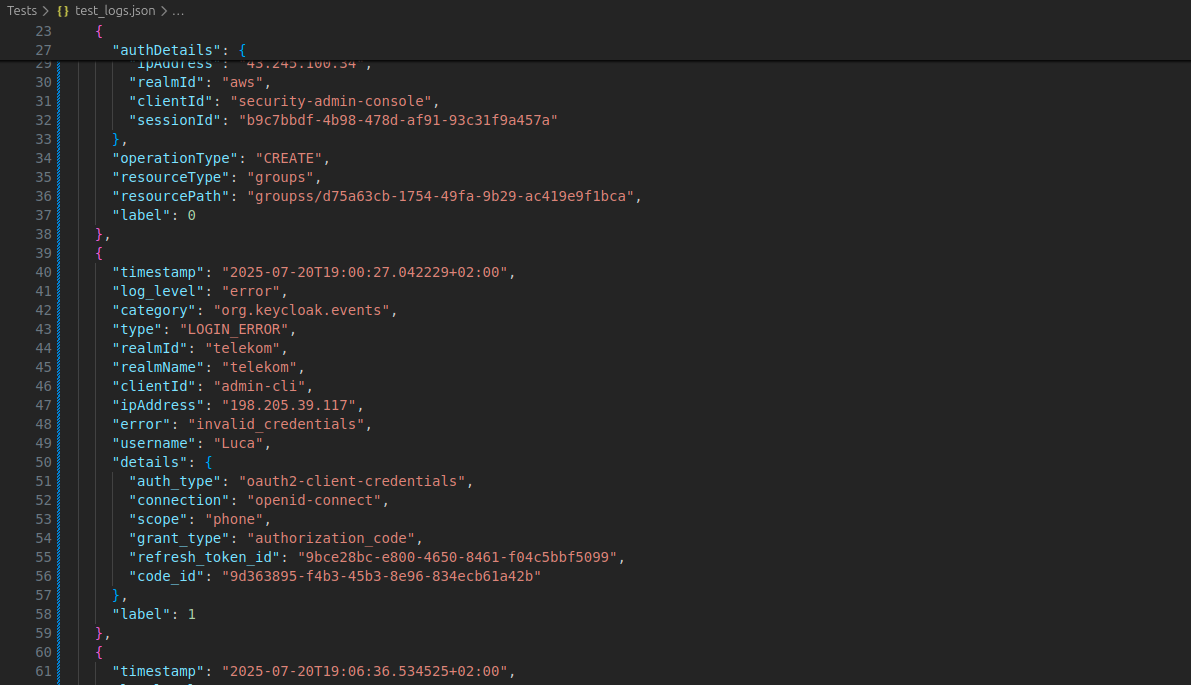
\includegraphics[width=1.0\linewidth]{Bilder/screenshot009}
		\caption{Ausschnitt der generierten Logs, Man erkennt hier schon ein Log mit dem Label 0, also ein normaler Log, unterhalb ist eines mit dem Label 1- eine Anomalie. Man erkennt hier schon den Typ LOGIN\_ERROR.}
		\label{fig:screenshot009}
	\end{figure}
	Bei der Generierung der Log-Daten wurde auch berücksichtigt, dass neben eindeutig normalen und anomalen Sessions auch uneindeutige Sequenzen erzeugt werden, die als \textit{\gls{noise}} klassifiziert werden können. Solche Fälle treten in realen Systemen häufig auf – etwa wenn ein normaler Nutzer temporär priorisierte Rollen übernimmt oder häufig Passwörter ändert, ohne dass ein tatsächlicher Angriff vorliegt. Um eine zu starke Sensitivität der Modelle gegenüber solchen Mustern zu vermeiden, wird bewusst ein gewisser Anteil an Rauschen erzeugt.

	\subsection{Grenzen dieser Lösung}
	Die Analyse basierte ausschließlich auf den wichtigsten, verfügbaren Log-Daten, die bekannte Systemaktivitäten und deren Merkmale widerspiegeln. Durch diesen Ansatz hat man die Kontrolle über die Logs und wie viele ca. erzeugt werden. Eine tiefere Untersuchung der internen Struktur und des vollständigen Aufbaus der Event-Typen in Keycloak war aufgrund fehlender umfassender Dokumentation und eingeschränktem Zugriff auf administrative Systemressourcen nicht möglich. Diese Einschränkungen begrenzen die Tiefe und Genauigkeit der Auswertung und können die Aussagekraft der Ergebnisse beeinflussen.
	\\[0.5em]
	Eine zentrale Herausforderung bestand in der realistischen Modellierung anomaler Sessions. Dabei musste unterschieden werden, ob eine Session normal, anormal oder als sogenannter Noise einzustufen ist, also als legitimes, aber ungewöhnliches Verhalten, das fälschlich als Anomalie interpretiert werden könnte. Da echte Anomalien in der Realität selten auftreten, wurde bei der Datengenerierung heuristisch eine Auftrittswahrscheinlichkeit von 2,\,\% für anomale Sessions angenommen. Dadurch ist nicht gewährleistet, dass die erzeugten Daten eine realistischere Verteilung widerspiegeln.
	\\[0.5em]
	Ein weiterer Nachteil der synthetischen Generierung liegt darin, dass zufällig zusammengesetzte Ereignismuster entstehen können, die keinem realistischen Angriff entsprechen. Um dem entgegenzuwirken, wurde eine Logik implementiert, die grundlegende Systemregeln von Keycloak berücksichtigt: So darf ein Benutzer mit eindeutiger ID nur in einem Realm existieren, es gibt jeweils nur einen Administrator mit explizit definierten Rollen und höherer Priorität, und normale Benutzer können keine Operationen ausführen, die mit dem Attribut \textit{operationType} (CRUD-Operationen) verbunden sind — diese bleiben ausschließlich Administratoren vorbehalten. Zudem wird sichergestellt, dass jeder Benutzer genau einer Session und einem Realm zugeordnet ist, sofern es sich nicht explizit um einen Angreifer handelt.
	\\[0.5em]
	Aufgrund dieser Einschränkungen sowie der im späteren Verlauf beobachteten Resultate wurde der vorgestellte Ansatz verworfen. Die Ergebnisse waren dabei sehr gut, was auch daran lag, dass mehr Anomalien erzeugt wurden, als in der Realität auftreten würden. Zudem können durchaus Logs bis 100.000 generiert werden. Für diesen Fall wurden auch längere Sequenzlängen verwendet und der LSTM-AE wurde sozusagen mit mehr Daten trainiert, wie es in der Praxis üblich ist.
	
	\section{Zweiter Ansatz: Manuelle Log-Generierung und durch Selenium}
	Wegen den zuvor genannten Nachteilen am ersten Ansatz, wurde stattdessen ein sinnvollerer Ansatz gewählt: Die Daten werden direkt aus dem Keycloak-System erhoben, um reale Anwendungsfälle abzubilden. Es wurde die Idee verfolgt, eine lokale Keycloak-Instanz aufzusetzen und von dieser Instanz aus die Logs zu erheben und zu nutzen. Dazu müssen die Logs jedoch manuelle erstellt werden. Da auch dieser Weg zeitintensiv ist, wurde zusätzlich erwogen, mittels sogenannter \gls{selenium}-Tests sowohl Angriffsszenarien als auch gewöhnliche Keycloak-Daten zu simulieren.So durch konnten viel schneller Logs erzeugt werden und es wurde viel Arbeitsaufwand erspart.Eine manuelle Durchführung wäre praktisch nicht möglich gewesen, da man dafür mehrere Benutzer gebraucht hätte, die diese Instanz nutzen und auch dabei täglich. Durch Selenium wurde gewährleistet, dass man immer noch Kontrolle darüber hat, welche Logs generiert werden und wie viele. Als Grundlage zur Definition normaler Keycloak-Logs dient dabei eine Orientierung an firmeninternen Log-Daten. Somit wird auch vermieden sensible Kundendaten (also Keycloak-Logs aus Keycloak-Instanzen der Kunden) zu erheben.
	
	\subsection{Anbindung der Keycloak-API}
	Um Zugriff auf die Keycloak-Logs zu erhalten, ist es erforderlich, eine eigene Keycloak-Instanz zu installieren und sich mit Administratorrechten anzumelden. Die Standard-Werte sind dafür als Benutzername sowie Passwort "admin".
	\\[0.5em]
	Der Zugriff auf die Event-Logs erfolgt über die Keycloak-API, welche insbesondere bei der verwendeten Quarkus-Distribution eingesetzt wird. Standardmäßig benötigt man hierfür entsprechende Administrator-Rollen, um sensible Informationen wie User-Event-Logs und Admini
	-Event-Logs abrufen zu können. Zunächst müssen die korrekten Authentifizierungsdaten vorliegen, um die erforderlichen Zugriffsrechte zu erhalten.
	\\[0.5em]
	Für die Authentifizierung wurde der sogenannte \textit{Client Credentials} Grant-Typ gewählt. Dabei erfolgt die Anmeldung über einen registrierten Client, wobei neben dem Client-Secret weitere Zugangsdaten übermittelt werden.

	\begin{figure}[H]
		\centering
		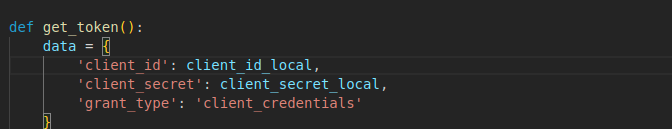
\includegraphics[width=0.9\linewidth]{Bilder/screenshot010}
		\caption{Daten, die an den Keycloak-Server gesendet werden müssen}
		\label{fig:screenshot010}
	\end{figure}
	Durch diesen Vorgang wird ein Zugriffstoken generiert, welches für den Abruf der Event-Logs benötigt wird. Das Token enthält Informationen zu den Zugriffsrechten des jeweiligen Admins. So müssen beispielsweise die Rechte zum Verwalten von Benutzern enthalten sein (also manage-users), damit diese auch im Token ausgewiesen werden. Ebenfalls benötigt amn die Berechtigung überhaupt auf Events zugreifen zu dürfen. Dafür wurde dem Admin die Rolle \gls{viewevents} zugeteilt. Anschließend wird mit diesem Token eine weitere Anfrage an die API gestellt, um die Event-Logs abzurufen. Die erhaltenen Daten werden in einer separaten JSON-Datei gespeichert.
	\\[0.5em]
	Weitere Details zur Keycloak-API sind in der offiziellen Dokumentation zu finden\footnote{Keycloak Documentation, „REST API Reference“, \url{https://www.keycloak.org/docs-api/latest/rest-api/index.html}, letzter Zugriff am 28.August.2025}.

	\subsection{Datenbeschaffung durch Selenium}
	Selenium \footnote{\url{https://www.selenium.dev/}, letzter Zugriff am 28.August.2025} ist ein Testframework zur automatisierten Ausführung von Webbrowser-Aktionen und als Python-Paket verfügbar. Es ermöglicht, Interaktionen mit der Benutzeroberfläche realitätsnah zu simulieren, sodass der Eindruck entsteht, ein Mensch bediene den Browser. Die wesentlichen Komponenten sind:
	
	\begin{itemize}
		\item \textbf{Selenium \gls{webdriver}}: Steuert den Browser programmgesteuert und stellt das zentrale Element der Tests dar.
		\item \textbf{Selenium Grid}: Ermöglicht die parallele Ausführung von Tests auf verschiedenen Maschinen und Browsern.
		\item \textbf{Selenium IDE}: Ein Recording-Tool im Browser, das jedoch für produktive oder komplexe Tests nicht empfohlen wird.
	\end{itemize}
	Für die Erstellung der Logs wird ausschließlich der WebDriver verwendet, der automatisch Chrome als Browser startet. Da Selenium anwendungsagnostisch ist, war das Steuern von Keycloak damit besonders leicht. Die Einrichtung gestaltet sich einfach: Es wird der zu verwendende Browser („Driver“) definiert und die Tests werden auf dem Port ausgeführt, auf dem die lokale Keycloak-Instanz erreichbar ist.
	\\[0.5em]
	Ein Nachteil dieser Methode liegt in der konstanten IP-Adresse, da alle Anfragen vom selben Host ausgehen. Dies kann dazu führen, dass das Modell lernt, mehrere Benutzer mit einer gemeinsamen IP-Adresse zu assoziieren, was in realen Szenarien als Anomalie interpretiert werden könnte. Daher wird die IP-Adresse vor der Weiterverarbeitung aus den Events entfernt. Diese Maßnahme reduziert zwar eine potenzielle Störquelle, verringert jedoch auch die Datenvielfalt für das Modell. Jedoch bestehen weiterhin genug Features, mit denen die Modelle arbeiten können, wie bspw. dem Event-Typen.
	\\[0.5em]
	Zudem erfolgt die Log-Erzeugung in kurzen zeitlichen Abständen, wodurch die zeitliche Streuung reduziert wird. Dies kann die Fähigkeit der Modelle zur Anomalieerkennung einschränken. Zwar werden wenige Tests zu ungewöhnlichen Uhrzeiten durchgeführt (z.B. abends), jedoch wurden davon nicht zu viele durchgeführt, damit die Modelle nicht lernen, dass eine Uhrzeit außerhalb der gewöhnlichen Arbeitszeit "normal" ist.
	\\[0.5em]
	Trotz dieser Einschränkungen überwiegt der Vorteil, dass die durch Selenium erzeugten Logs den realen Keycloak-Logs sehr nahekommen – ein zentraler Aspekt, insbesondere wenn wirtschaftlich verwertbare Erkenntnisse aus dieser Arbeit gewonnen werden sollen. Da die Logs direkt durch die definierten Tests erzeugt und gespeichert werden, entfällt die Notwendigkeit einer separaten manuellen Log-Generierung größtenteils.

	Zur Generierung der normalen Trainingsdaten wurden zuvor vier Realms erstellt:
	
	\begin{itemize}
		\item ubisoft
		\item Nintendo
		\item Sega
		\item aws
	\end{itemize}
	
	Pro Realm erfolgt die Benutzeranmeldung über einen jeweils definierten Client. Absichtlich wurden keine Benutzer und Clients im Master-Realm erzeugt, da auf diesen standardmäßig andere Admins aus den Nicht-Master-Realms nicht zugreifen können. Durch das Weglassen des Master-Realms bei der Generierung normaler Benutzerlogs wurde sichergestellt, dass die aufgezeichneten Logs ausschließlich reale Benutzeraktivitäten aus den einzelnen Realms widerspiegeln, ohne dass administrative Operationen oder systeminterne Aktionen die Analyse verfälschen. Dies erhöht die Klarheit und Vergleichbarkeit der Anomalieerkennung, da nur typische Nutzerinteraktionen untersucht werden und auch nur die der internen Admins in den einzelnen Realms.
	\\[0.5em]
	Im Realm \textit{ubisoft} wurden 25 synthetische Benutzer erstellt, deren Namen alphabetisch generiert wurden (jeder Buchstabe des Alphabets außer „X“ ist vertreten, da dafür kein Name gefunden wurde). Für diesen Realm wurde der Client \textit{ps3} angelegt. Dieser ist erforderlich, damit sowohl Admins Zugriff auf die User-Events erhalten als auch Benutzer sich über diesen Client authentifizieren können.
	\\[0.5em]
	In den weiteren Realms – \textit{Sega}, \textit{Nintendo} und \textit{aws} – wurden jeweils zehn Benutzer angelegt. Die zugehörigen Clients lauten: \textit{megadrive} (Sega), \textit{wii} (Nintendo) und \textit{aws-console} (aws).
	\\[0.5em]
	Jeder Realm verfügt über genau einen Admin mit der Rolle \textit{realm-admin}. Ein Admin, der für einen bestimmten Client Benutzer anlegen oder verwalten möchte, benötigt darüber hinaus die Rollen \textit{manage-users} und \textit{view-events}. Wichtig ist hierbei, dass diese Rollen nicht direkt den Benutzern, sondern den jeweiligen Clients zugewiesen werden. Dies liegt in der Architektur von Keycloak begründet: Clients besitzen eigene Zugriffsrechte, die ihnen bestimmte Operationen ermöglichen. So erlaubt die Rolle \textit{manage-users} dem Client, Benutzer im Realm programmatisch zu verwalten, während \textit{view-events} erforderlich ist, um Zugriff auf die Ereignisprotokolle zu erhalten – essenziell für Logging und Fehlersuche.
	\\[0.5em]
	
	\begin{figure}[H]
		\centering
		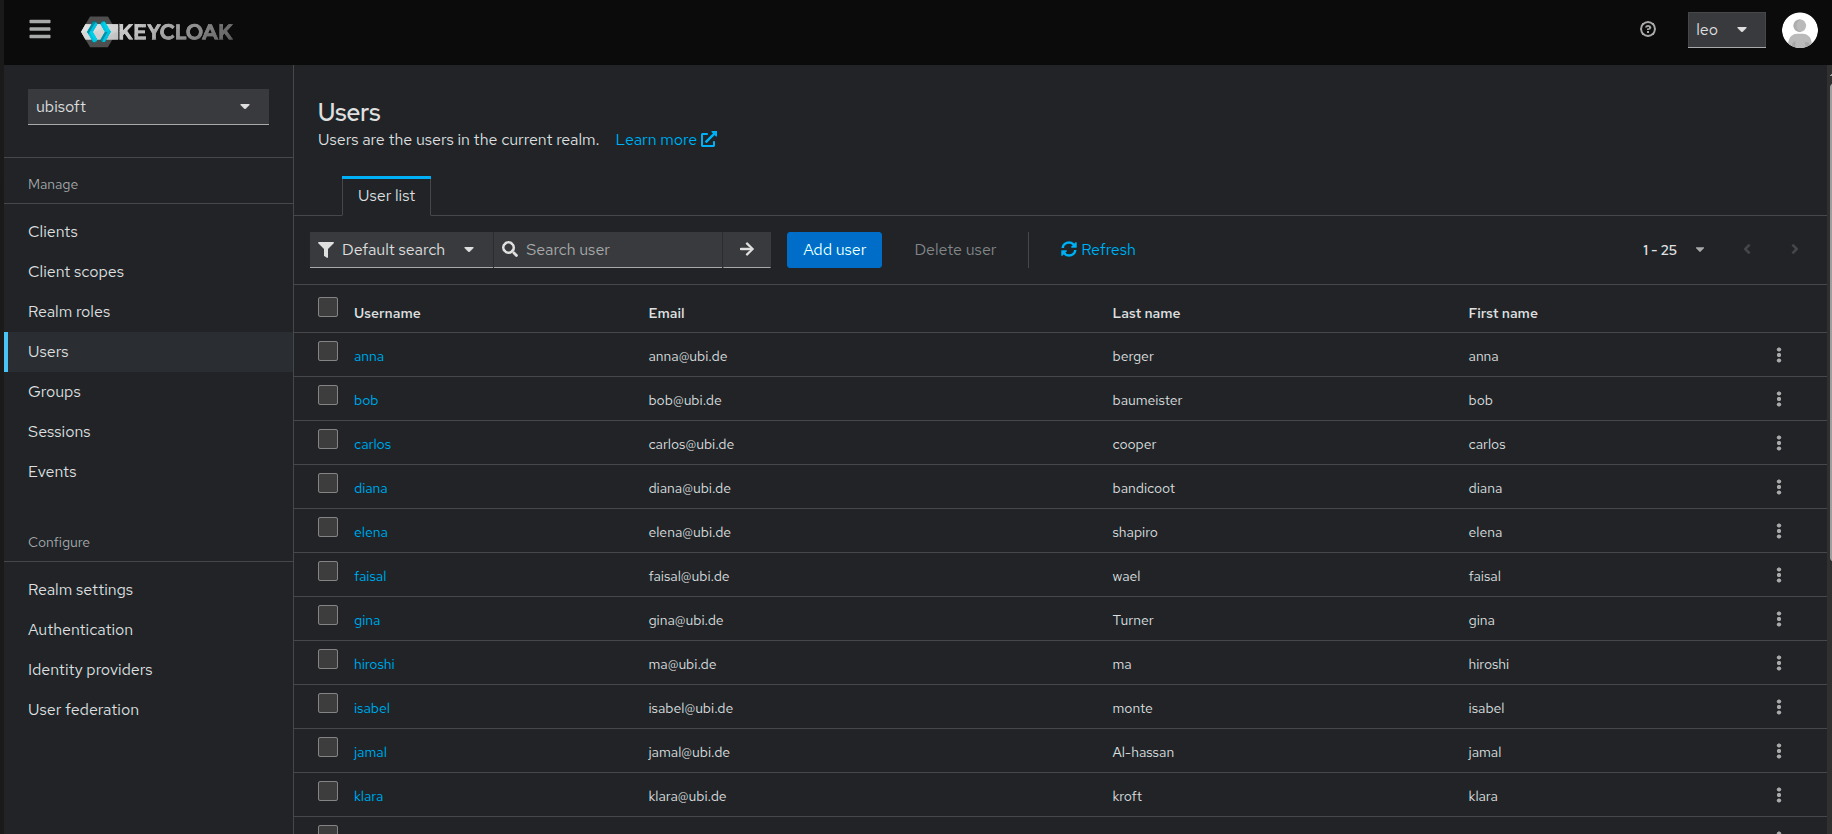
\includegraphics[scale=1.5, width=\linewidth]{Bilder/screenshot011}
		\caption{Beispielhafte Darstellung der generierten Benutzer für den Testfall}
		\label{fig:screenshot011}
	\end{figure}
	
	Im Rahmen dieser Arbeit erzeugt ein Selenium-Test automatisch neue Benutzerkonten in Keycloak und weist ihnen jeweils ein Passwort zu. Diese Daten werden pro Realm einmalig in einer \gls{jsonl}-Datei gespeichert, wobei Benutzername und Passwort als Schlüssel-Wert-Paar abgelegt werden.
	\\[0.5em]
	Damit sich die erzeugten Benutzer über die automatisierten Tests in Keycloak anmelden können, muss in der Konfiguration festgelegt werden, dass ein vollständiges Profil (Vorname, Nachname, E-Mail) erforderlich ist und vorhanden ist– andernfalls würde die Authentifizierung fehlschlagen.
	\\[0.5em]
	Darüber hinaus verfügen Clients dann über Service Accounts. Die Service-Account-Rollen bestimmen dabei die verfügbaren Rechte. Ohne diese Rollen könnte der Client zwar eine Verbindung herstellen, hätte jedoch keinen Zugriff auf Benutzerverwaltung oder Logdaten. Die korrekte Konfiguration der Service-Account-Rollen ist daher zwingend notwendig, um automatisierte Vorgänge im Hintergrund zu ermöglichen.
	
	\begin{figure}[H]
		\centering
		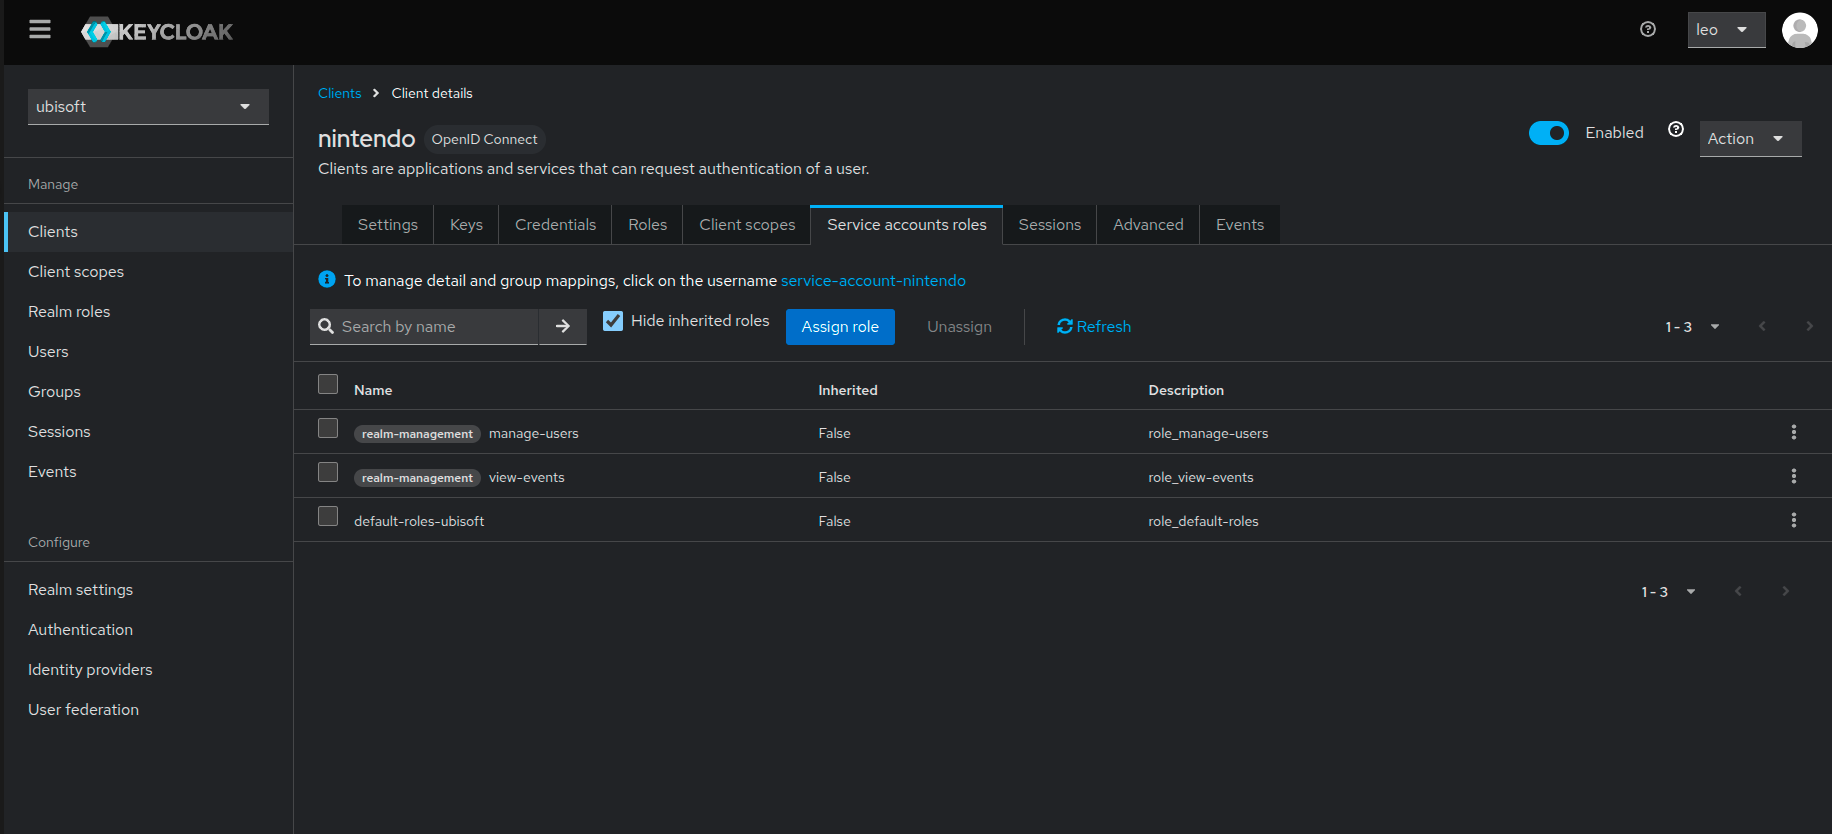
\includegraphics[width=0.9\linewidth]{Bilder/screenshot012}
		\caption{Benötigte Rollen für den Client Nintendo}
		\label{fig:screenshot012}
	\end{figure}
	Ab einer bestimmten Menge an Trainingsdaten werden die generierten Benutzer im Rahmen des Selenium-Tests dazu gebracht, sich regulär anzumelden. Die dabei entstehenden sogenannten „gewöhnlichen“ Logs umfassen unter anderem Anmeldevorgänge und sind wie bereits erwähnt, inspiriert von realen firmeninternen Protokollen. Diese bestehen typischerweise aus den Event-Typen LOGIN, CLIENT\_LOGIN und CODE\_TO\_TOKEN.
	\\[0.5em]
	Folgende Aktivitäten gelten laut interner Log-Analyse als „typisch“ nach einen Vergleich mit den firmeninternen Keycloak-Logs:
	
	\begin{itemize}
		\item Anmeldung über einen Client
		\item Token-Aktualisierung (\gls{refresh_token})
		\item Abmeldung (Logout), auch nach Ablauf einer Session
		\item Fehlgeschlagene Login-Versuche (kommen häufiger vor)
	\end{itemize}
	Weitere Aktionen – wie das Anpassen des Benutzerprofils (z. B. E-Mail-Änderung, Passwort-Zurücksetzung), das Löschen eines Clients oder das Zuweisen von Rollen an andere Benutzer beziehungsweise Clients – wurden in der Log-Generierung bewusst manuell durchgeführt. Der Grund hierfür liegt in der vergleichsweise hohen Komplexität und der geringen Häufigkeit dieser Vorgänge. Da Keycloak primär als SSO-Dienst genutzt wird, wäre eine regelmäßige Durchführung solcher Aktionen im automatisierten Testkontext unrealistisch und würde die Aussagekraft der „normalen“ Logs verzerren.
	\\[0.5em]
	Stattdessen werden solche seltenen Aktionen manuell während des Testbetriebs von einzelnen Benutzern durchgeführt. Um dabei in die „Rolle“ eines anderen Benutzers zu schlüpfen, wird der Event-Typ \gls{impersonate} verwendet. Die Verwendung von Impersonation während der automatisierten Testausführung wird vermieden, da sie eine potenzielle Anomalie darstellt. Ziel ist es, lediglich gelegentlich und gezielt ungewöhnliche Aktionen zu erzeugen – etwa eine Passwort- oder E-Mail-Änderung, das Anlegen oder Löschen eines Benutzers oder das Zuweisen von Rollen. Dies reduziert den manuellen Aufwand bei der Erzeugung seltener Ereignisse, ohne die Gesamtdatenbasis zu verzerren.
	\\[0.5em]
	Pro Durchlauf werden insgesamt 30 Sessions (Bei den ersten 10000 Loggs waren es noch 15, wurde aber erhöht, um schneller Logs zu erzeugen) durchgeführt, wobei jede Session durch den häufigen Einsatz von Refresh Tokens mindestens zehn Einträge im Log erzeugt. Die Sitzungsdauer wird dabei durch die Konfiguration des jeweiligen Realms bestimmt. Aus praktischer Erfahrung ergibt sich eine durchschnittliche Dauer von etwa 35 Minuten pro Session – realistisch im Rahmen von 10 Minuten bis zu einer Stunde. So können am Tag zwischen 2.500 und 5.000 Log-Einträge erzeugt werden.
	\\[0.5em]
	Ereignisse, die typischerweise erst nach längerer Zeit auftreten, fehlen somit in der Testbasis. Eine spätere Erweiterung ist möglich, jedoch wurde aufgrund der Bearbeitungsfrist beschlossen, die Generierung auf 12 aufeinanderfolgende Tage zu konzentrieren, ausgeschlossen ist dabei das Wochenende. Die Sessions werden dabei nacheinander mit variablen Abstand ausgeführt.
		
	\subsection{Mögliche Angriffszenarien basierend auf CVE und CWE}
	\gls{cve} stellt eine umfassende Datenbank bekannter Sicherheitslücken dar, die in verschiedenen Softwaresystemen dokumentiert sind. Für Keycloak existieren ebenfalls zahlreiche veröffentlichte Schwachstellen\footnote{MITRE Corporation, „CVE Search Results for Keycloak“, \url{https://cve.mitre.org/cgi-bin/cvekey.cgi?keyword=keycloak}, letzter Zugriff am 28.August.2025}.
	\\[0.5em]
	CVE-Einträge liefern jedoch keine Lösungen, sondern dienen der Information über Art, Ursache und potenzielle Auswirkungen der jeweiligen Sicherheitslücke. Jeder Eintrag erhält eine eindeutige Identifikationsnummer, eine Kurzbeschreibung sowie (sofern verfügbar) Angaben zur betroffenen Softwareversion. Die Pflege und Dokumentation erfolgt weltweit durch Organisationen, Forschungseinrichtungen sowie unabhängige Sicherheitsexperten.
	\\[0.5em]
	Im Gegensatz dazu beschreibt die \gls{cwe} systematisch bekannte Schwachstellenmuster (Weaknesses), die potenziell zu Sicherheitslücken führen können. Während CVEs konkrete, bereits gefundene oder ausgenutzte Schwachstellen auflisten, klassifiziert CWE abstrakte Fehlerklassen, wie beispielsweise „unzureichende Rechteprüfung“ oder „unsichere Tokenverarbeitung“. Beide Kataloge sind essentiell für die systematische Entwicklung und Interpretation von Sicherheitstests.
	\\[0.5em]
	Obwohl viele der bekannten Probleme bereits behoben wurden, zeigen sich Schwachstellen in Keycloak zunehmend wiederkehrend und entwickeln sich mit der Zeit weiter. In letzten Versionen bspw. können zwar frühere Schwachstellen behoben worden sein, in späteren jedoch neue Schwachstellen und Lücken auftreten.
	\\[0.5em]
	Im Rahmen dieser Arbeit wurden mittels Selenium gezielt sicherheitsrelevante Angriffszenarien nach CVE und CWE und anderen Quellen (die schon im vorherigen Kapiteln bzgl. des ersten Entwurfes der Angriffsszenarien beschrieben wurden), gegen Keycloak simuliert und getestet. Es wird dabei folgendes Angriffsszenario zur Orientierung genommen: 
	\\[0.5em]
	\textbf{CVE-2024-3656 - \gls{privilegeescalation} in Keycloak}
	Bei CVE-2024-3656\footnote{CVE-Ticket: \url{https://www.cve.news/cve-2024-3656/}, letzter Zugriff am 28.August.2025} handelt es sich um eine Sicherheitslücke in Keycloaks Admin REST API, bei der unzureichende Berechtigungsprüfungen es einem Nutzer mit niedrigen Rechten ermöglichen, administrative Endpunkte aufzurufen. Dadurch können sensible Daten wie Benutzerlisten eingesehen und administrative Aktionen durchgeführt werden, ohne dass entsprechende Rechte vorliegen. Die Ursache liegt in fehlerhaften oder fehlenden Zugriffskontrollen auf kritischen API-Endpunkten. Die Schwachstelle wurde in neueren Keycloak-Versionen behoben, darunter auch die Version 26.1.0, welche in dieser Arbeit verwendet wird. Andere Angriffsfälle konnten nicht umgesetzt werden, da manche Features die dafür verlangt werden in aktuellen oder früheren Versionen nicht mehr erhältlich sind. Auch wenn dieser Angriff fehlschlägt, sorgt er dafür, dass viele Logs mit anomalen Charakter generiert werden.
	\\[0.5em]
	Da CVE-Datenbanken keine vollständigen Exploitbeschreibungen liefern, wurde im Rahmen der Simulation eine technische Interpretation der Schwachstellen vorgenommen. Zudem wurden noch weitere Angriffe ausgeführt, welche typisch sind für einen Angriff und auch schon in den bekannten Insiderangriffsfällen genannt wurde:
	\begin{itemize}
		\item \textbf{\gls{accountsabotage}-Test: }  
		Löschen oder Verändern wichtiger Benutzerinformationen.
		\item \textbf{Dictionary Angriff}
	\end{itemize}

	\subsection{Angriffsszenarien}                         
	Die im vorherigen Abschnitt beschriebenen Angriffsszenarien wurden im Rahmen dieser Arbeit mithilfe von Selenium-Tests implementiert und in den generierten Logs dokumentiert. Für jedes Szenario wurde ein konkreter Ablauf definiert, um die jeweilige Sicherheitslücke zu simulieren.
	\\[0.5em]
	Hier werden die Angriffsfälle aufgelistet welche direkt in der Keycloak-Konsole ausgeführt wurden, also nicht als Selenium-Test- außer das erste Szenario des Testfalls \textit{Privilege Escalation}, dieses wird auch als Selenium-Test ausgeführt.
	
	\subsubsection{Privilege Escalation}
	In diesem Szenario wird untersucht, ob ein technisch privilegierter, aber nicht vollständig administrativer Benutzer in Keycloak durch gezielte API-Aufrufe seine eigenen Berechtigungen ausweiten kann. Ziel ist es, das Verhalten von Keycloak bei einer möglichen Rechteausweitung über die REST-Schnittstelle zu evaluieren.
	
	\begin{figure}
		\centering
		\includegraphics[width=0.3\linewidth]{Bilder/priv\_esc\_ad}
		\caption{Aktivitätsdiagramm Privilege Escalation}
		\label{fig:privescad}
	\end{figure}
	
	
	\begin{description}
		\item[Ziel:] Unautorisierte Erweiterung der Benutzerrechte durch Ausnutzung der REST API
		\item[Betroffener Realm:] \texttt{ubisoft}
		\item[Angreiferrolle:] Benutzer mit der Rolle \texttt{manage-users}
		\item[Betroffener Benutzer:] \texttt{bob} (versucht sich selbst administrative Rechte zu geben)
	\end{description}
	
	\paragraph{Ablauf:}
	\begin{enumerate}
		\item Der Benutzer \texttt{bob} meldet sich regulär im System an und verfügt über ein gültiges Access Token.
		\item Mit diesem Token führt er einen \texttt{GET}-Request auf \texttt{/admin/realms/ubisoft/users} aus, um die Benutzerliste des Realms zu erhalten.
		\item Die Abfrage ist erfolgreich – bob erhält Zugriff auf die vollständige Liste und identifiziert seine eigene Benutzer-ID.
		\item Anschließend versucht er über einen \texttt{POST}-Request 
		an 
		\textit{/admin/realms/ubisoft/users/\{id\}/role-mappings/realm}, 
		sich selbst die Rolle \texttt{realm-admin} zuzuweisen.
		\item Der Request schlägt fehl – die Serverantwort ist \texttt{HTTP 403 Unauthorized}.
	\end{enumerate}
	
	\paragraph{Technische Umsetzung:}
	Die Requests wurden mithilfe von \texttt{curl} direkt an die REST API gesendet. Dabei wurde ein korrekt signiertes Access Token verwendet, das bob durch einen Login mit seiner \texttt{manage-users}-Rolle erhalten hatte.
	
	\paragraph{Erwartetes Verhalten:}
	\begin{itemize}
		\item Die Benutzerliste kann durch Rollen wie \texttt{manage-users} teilweise eingesehen werden, was ein potenzielles Datenschutzrisiko darstellt.
		\item Die unautorisierte Zuweisung privilegierter Rollen wird vom Server korrekt abgelehnt.
		\item Der Zugriff auf administrative Rollen über die REST API ist in Keycloak Version 26.1 restriktiver als in früheren Versionen, was diese Art von Privilege Escalation wirksam verhindert.
	\end{itemize}


	\subsubsection{Angriffsszenario: Account-Sabotage durch privilegierten Benutzer}
	In diesem Szenario wird untersucht, inwieweit ein privilegierter Benutzer (z.\,B. ein Administrator) absichtlich oder versehentlich Schaden an Benutzerkonten anrichten kann. Ziel ist es, das Verhalten von Keycloak bei kritischen administrativen Operationen zu beobachten und zu analysieren, welche Aktionen protokolliert werden.
	
	\begin{figure}
		\centering
		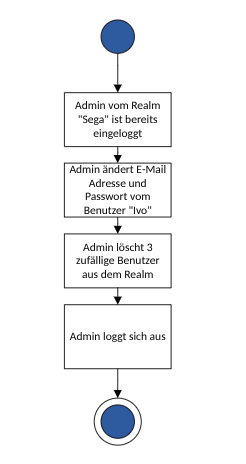
\includegraphics[width=0.3\linewidth]{Bilder/angriff_2}
		\caption{Aktivitätsdiagramm von Account-Sabotage}
		\label{fig:angriff2}
	\end{figure}
	
	\begin{description}
		\item[Ziel:] Simulierte Account-Sabotage durch einen legitimen Admin im Realm
		\item[Betroffener Realm:] \texttt{Sega}
		\item[Angreiferrolle:] Benutzer mit Administratorrechten (z.\,B. \texttt{realm-admin} oder \texttt{manage-users})
		\item[Betroffene Benutzer:] \texttt{Admin in Sega} (Profiländerung) sowie drei zufällige Benutzer (Löschung)
	\end{description}
	
	\paragraph{Ablauf:}
	\begin{enumerate}
		\item Ein Angreifer kennt die Credentials des Admins im Realm \texttt{Sega} und ist bereits mit dessen Credentials eingeloggt.
		\item Der Angreifer ändert das Passwort des Admins in Sega.
		\item Anschließend löscht der Admin drei beliebige Benutzerkonten im selben Realm.
		\item Der Angreifer meldet sich ab.
	\end{enumerate}
	
	\paragraph{Technische Umsetzung:}
	Die Ausführung erfolgt entweder manuell über die Keycloak Admin Console oder automatisiert mit Hilfe von \texttt{Selenium}.
	
	\paragraph{Erwartetes Verhalten:}
	\begin{itemize}
		\item Die Profiländerungen und das Zurücksetzen des Passworts sollten als \texttt{UPDATE\_PASSWORD} im \textbf{User-Event-Log} erscheinen.
		\item Die Löschung der Benutzerkonten wird im \textbf{Admin-Event-Log} als \texttt{DELETE} Operation registriert.
		\item Alle Aktionen sind über den Zeitstempel, Benutzer und IP-Adresse nachvollziehbar.
		\item \textit{LOGOUT} wird ebenfalls in den Logs angezeigt
	\end{itemize}
	
	Das einzige Szenario, welches durch ein Selenium-Test erzeugt wurde ist folgendes:

	\subsubsection{Angriffsszenario: Dictionary-Angriff über die Web-Oberfläche}
	In diesem Szenario wird ein klassischer Dictionary-Angriff simuliert, bei dem ein Benutzername fest vorgegeben ist und systematisch unterschiedliche Passwörter ausprobiert werden. Ziel ist es zu prüfen, ob ein erfolgreiches Login durch mehrfaches Raten von Passwörtern möglich ist und ob Keycloak entsprechende Fehlversuche protokolliert.
	
	\begin{figure}
		\centering
		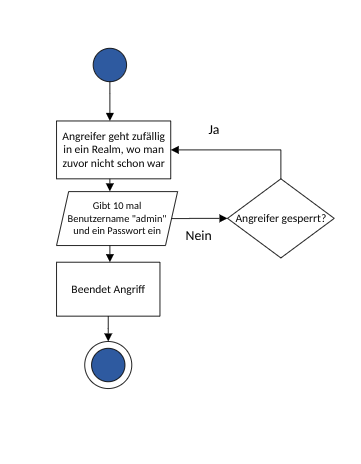
\includegraphics[width=0.4\linewidth]{Bilder/angriff_3}
		\caption{Aktivitätsdiagramm von Dictionary}
		\label{fig:angriff3}
	\end{figure}
		
	\begin{description}
		\item[Ziel:] Test der Account-Sicherheit gegenüber einfachen Dictionary-Angriffen über das Login-Formular
		\item[Betroffener Benutzer:] \texttt{Admin}
		\item[Realm:] Dynamisch gewählt (aus mehreren Realms auswählbar)
		\item[Passwortliste:] Eine Liste gängiger schwacher Passwörter (z.\,B. \texttt{admin123}, \texttt{123456}, \texttt{password}, \texttt{qwerty}, \texttt{welcome}, etc.)
	\end{description}
	
	\paragraph{Ablauf:}
	\begin{enumerate}
		\item Es wird eine Verbindung zur Keycloak-Login-Seite des jeweiligen Realms hergestellt.
		\item Der Benutzername wird in das Formular eingetragen (\texttt{Admin}).
		\item Es wird nacheinander jedes Passwort aus der vorgegebenen Liste eingegeben und die Login-Schaltfläche betätigt. Wenn Keycloak angibt, dass zu viele fehlgeschlagene Anmeldeversuche versucht wurden, wechselt der Angreifer die Login-Startseite des jeweiligen Realms (Pro Realm gibt es unterschiedliche Login-Startseiten, bei der in der URL ein anderes Realm steht)
		\item Das Skript prüft, ob eine Fehlermeldung erscheint oder ob der Login erfolgreich war.
		\item nach 10 gescheiterten versuchen wird das Szenario, bzw. Skript gestoppt.
	\end{enumerate}
	
	\paragraph{Technische Umsetzung:}
	Die Automatisierung erfolgt mittels \texttt{Selenium WebDriver} in Kombination mit einer Python-Testfunktion. Die Login-Seite wird jeweils mit einem neuen Passwort geladen und automatisiert ausgefüllt.
	
	\paragraph{Erwartetes Verhalten:}
	\begin{itemize}
		\item Keycloak sollte nach mehreren Fehlversuchen Gegenmaßnahmen ergreifen (z.\,B. Account-Sperrung, Rate Limiting).
		\item Im Event-Log sollten die fehlgeschlagenen Login-Versuche als \texttt{LOGIN\_ERROR} mit dem jeweiligen Benutzer verzeichnet sein.
	\end{itemize}
	
	Dictionary und Privilege Escalation sind Angriffe, die fehlschlagen. Nur Account- Sabotage ist erfolgreich. Dies liegt an der Umsetzung (Dictionary Angriff durch Selenium-Tests) und daran, dass der erwähnte CVE Fall für neuere Keycloak Versionen nicht mehr funktioniert durch neue Sicherheitsfunktionen- dennoch stellen sie erkennbare, anomale Logs dar.

	\subsection{Änderung der Timestamps durch Unix Timestamp}
	Die Angriffsszenarien wurden am Ende der 12 Tage, also am 12. Tag erzeugt. So durch wirkt es, als ob alle Angriffe am letzten Tag erzeugt worden sind. Dies verringert die zufällige Verteilung der Angriffe. Daher müssen die Timestamps manuell geändert werden. Es muss gewährleistet sein, dass diese zufällig vom 22.07, ca. 14 Uhr bis zum 08.08, 17 Uhr erzeugt wurden- und demnach verändert werden. Es wurden folgende Zeitpunkte pro Angriffsszenario modelliert:
	\begin{itemize}
		\item \textit{Dictionary Angriff:} Umstellung auf den 06.08 um 13 Uhr Abends
		\item \textit{Privilege Escalation:} Umstellung auf den 07.08 um 16 Uhr
		\item \textit{Account Sabotage:} Umstellung auf den 08.08 um 11 Uhr Morgens
	\end{itemize}
	Diese Zeitpunkte werden auf der Webseite Unix Timestamp\footnote{Unix Timestamp Umwandler: \url{https://www.unixtimestamp.com/}, letzter Zugriff am 28.August.2025} verändert.
	
	\begin{figure}[H]
		\centering
		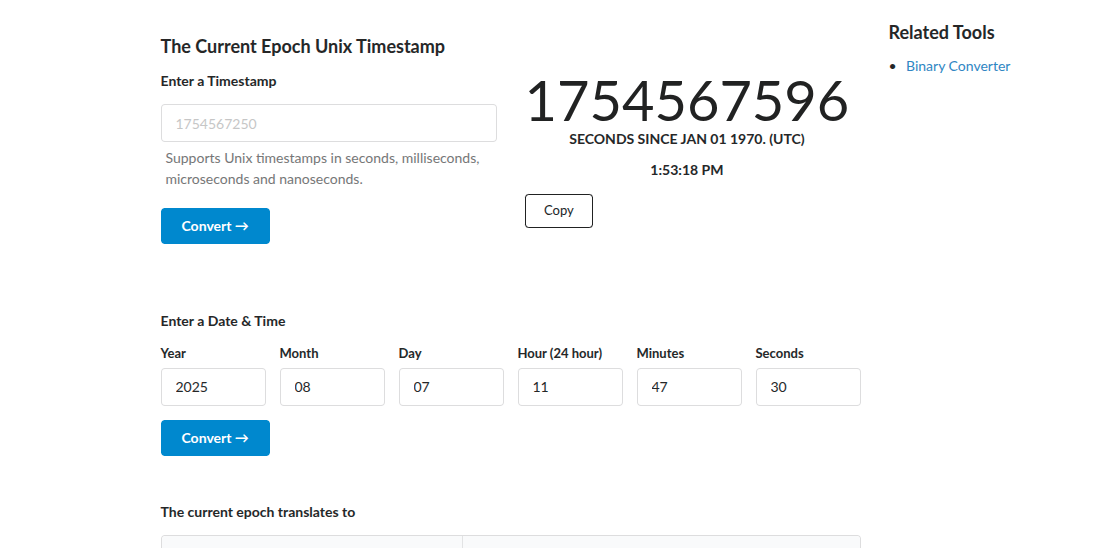
\includegraphics[width=0.9\linewidth]{Bilder/screenshot019}
		\caption{Aktuelle Uhrzeit nach dem Unix-System \textit{[Online]. Verfügbar unter:} \url{https://www.unixtimestamp.com/}, abgerufen am 18. August 2025.}
		\label{fig:screenshot019}
	\end{figure}
	
	Die erste Attacke dauert ca. 1-2 Minuten, die zweite ca. 5-10 Minuten und die letzte im ca. 20 Minuten. Dies Zeit wurde so bestimmt, dass sie sich für den jeweiligen Angriff eignen. Die Angriffe werden mit Absicht an Zeitpunkte durchgeführt, welche zwischen den normalen Logs mit Abstand sind, damit das LSTM-AE auch seinen Einsatz daran zeigen kann. 
	
	\section{Durchführung des Trainings}
	Die Logs werden separat je nach Training, Test und Validierung in Dateien gepackt und dann zu Beginn ausgelesen. Alle drei Dateien, also Evaluierungs-, Test- und Trainingsdateien werden dabei einzeln bereinigt und zusammengefügt. Darauf hin werden alle Daten mit der standardisiert und skaliert, wie im Abschnitt zur Implementierung bereits erklärt. Da der LSTM-AE nur mit sequentiellen Daten arbeiten kann, wurden diese Dateien in Sequenzen aufgeteilt.
	\\[0.5em]
	Über einen Zeitraum von 12 Tagen (ca. 2.5 Wochen, nur Werktage) wurden ausschließlich „normale“ Logs generiert. An den darauffolgenden Tagen fanden gezielte Angriffsszenarien statt. Mithilfe eines Skripts wurden anschließend sämtliche Event-Logs aus allen Realms zusammengeführt. 
	\\[0.5em]
	Das Skript funktioniert in etwas wie folgt:
	\\[0.5em]
	Die kombinierten Logs werden zunächst im Verhältnis 70\,\% zu Trainingsdaten und jeweils 15\,\% zu Test- und Validierungsdaten aufgeteilt. Die Anomalien werden zufällig auf die Test- und Validierungsdaten verteilt, dabei jedoch in chronologischer Reihenfolge einsortiert. Da die Anomalien erst nachträglich erzeugt wurden, mussten die Timestamps wie bereits diskutiert, entsprechend angepasst werden.
	\\[0.5em]
	Eine rein zufällige Vergabe der Timestamps war dabei nicht möglich, da bestimmte Angriffsszenarien einen klaren zeitlichen Ablauf erfordern. Die Timestamps wurden daher gezielt so angepasst, dass sie diesen inhaltlichen Zusammenhang korrekt abbilden, ohne bspw. am Ende des Datensatzes zu kumulieren. Aufgrund der überschaubaren Anzahl an Anomalien (ca. 31 Einträge) konnte dieser Schritt manuell umgesetzt werden. Die Logs wurden dennoch in chronologischer Reihenfolge angeordnet, sodass der zeitliche Ablauf der Ereignisse konsistent abgebildet wird.
	\\[0.5em]
	Die Anomalien sind zuvor in eine separate Datei ausgelagert. Bevor die anomalen Logs mit den normalen vermischt werden, fügt das Skript Labelinformationen hinzu: In der Datei \textit{attacks\_logs.py} wurden die anomalen Ereignisse aus Keycloak extrahiert und mit dem Label "1"  versehen, während in der Datei \textit{normal\_test\_logs.py} die regulären Log-Einträge mit dem Label "0"  markiert wurden.
	\\[0.5em]
	Abschließend wird die finale Datei in zwei Hälften aufgeteilt; in eine Validierung- und einer Testdatei.
	\\[0.5em]
	Das LSTM-AE wird ausschließlich mit normalen, nicht gelabelten Daten trainiert. Dies liegt an der Funktionsweise des Autoencoders, der lediglich versucht, die Eingangsdaten zu rekonstruieren. Nach ausreichendem Training lernt er, nur normale Daten zuverlässig zu rekonstruieren. Enthalten die Testdaten Anomalien, werden diese schlechter rekonstruiert, was zum sogenannten Rekonstruktionsfehler führt.
	\\[0.5em]
	Jedes Hybridmodell wurde pro Sequenzlänge fünfmal trainiert. Dies ist notwendig, um die durch die zufällige Initialisierung der Parameter in neuronalen Netzen bedingte stochastische Variabilität angemessen abzubilden.
	
	\subsection{Die Anzahl der Log-Einträge}
	Wie viele Trainingsdaten an sich auch nötig sind, ist ein weitgehend offenes Problem. Es gibt Studien, die sich systematisch mit der Frage beschäftigt haben, welche Datenmenge „angemessen“ ist, um ein neuronales Netzwerk zuverlässig zu trainieren. 
	\\[0.5em]
	Nach der Studie von Golestaneh et al. \cite{Golestaneh2021} wurde eine theoretische Fehlerabschätzung für bestimmte Netzwerke abgeleitet. Demnach skaliert der Fehler $\varepsilon$ eines solchen Netzwerks nicht mit der klassischen „parametrischen“ Rate von $\varepsilon \sim 1/n$, sondern mit einer langsameren Rate:
	
	\[
	\varepsilon(n) \sim \frac{1}{\sqrt{n}}
	\]
	Dabei ist \(n\) die Anzahl der Trainingsbeispiele. Diese Formel bedeutet, dass eine Verdopplung der Datenmenge den Fehler nicht halbiert, sondern nur um den Faktor \(1/\sqrt{2}\) verringert. Dennoch erlaubt diese Abschätzung eine grobe Einschätzung der notwendigen Datenmenge.
	\\[0.5em]
	Wendet man diese Formel auf eine Trainingsmenge von $n = 10.000$ Log-Zeilen an, ergibt sich ein theoretischer Fehler von etwa
	
	\[
	\varepsilon(10.000) \approx \frac{1}{\sqrt{10.000}} = 0{,}01
	\]
	Dieser Wert gilt zwar nicht als absolute Fehlermarke (da der tatsächliche Fehler von Modellarchitektur, Datenqualität und Regularisierung abhängt), er ist jedoch in vielen praktischen Fällen bereits hinreichend gering, um eine sinnvolle Modellierung zu ermöglichen. Somit kann ein LSTM-Autoencoder bei geeigneter Modellwahl und sauberem Datenvorverarbeitung bereits mit etwa 10.000 normalisierten Log-Zeilen ein brauchbares Modell für Anomalieerkennung liefern.
	\\[0.5em]
	Auch eine weitere Studie von Götz et al. \cite{Goetz2023} beschäftigt sich mit der Relation zwischen der Komplexität eines neuronalen Netzwerks (gemessen an der Anzahl der trainierbaren Parameter \( N_p \)) und der Anzahl der notwendigen Trainingsbeispiele \( N_{tr} \). Dabei wurde gezeigt, dass kein starres Verhältnis wie \( N_{tr} \geq N_p \) erforderlich ist, um gute Ergebnisse zu erzielen. Stattdessen weisen die Autoren nach, dass auch mit deutlich weniger Trainingsbeispielen eine stabile Modellleistung möglich ist.
	\\[0.5em]
	In ihren Experimenten mit Convolutional Neural Networks (CNNs) konnten selbst bei einem Verhältnis \( N_{tr}/N_p < 1 \) noch vergleichbare Klassifikationsleistungen erzielt werden, solange die Reduktion der Netzwerkkomplexität kontrolliert erfolgt. Übertragen auf den vorliegenden Fall bedeutet dies: Bei einem moderat komplexen LSTM-Autoencoder mit z.\,B. einigen zehntausend Parametern können bereits $10.000$ Trainingsbeispiele (z.\,B. Log-Zeilen) ausreichen, um ein funktionierendes Modell zu erhalten – sofern geeignete Regularisierung und Modellarchitektur verwendet werden. 
	\\[0.5em]
	Die Studie stützt damit ebenfalls die Annahme, dass in vielen praktischen Szenarien bereits Datensätze von 10.000 Einträgen als ausreichend gelten können, um eine robuste Anomalieerkennung durchzuführen- wobei man natürlich beachten muss, dass in jeder Studie der Fokus auf einem anderen Netzwerk lag. Dennoch will man diese Studien als Hinweis dafür wahrnehmen, möglichst viele Daten zu generieren, auch wenn es im Rahmen dieser Arbeit die Anzahl der wahrscheinlich nur im fünf-stelligen Bereich liegen wird.
	\\[0.5em]
	Auf Grundlage dieser Erkenntnisse wird eine Testdatei mit ca. 5.850 Logs erstellt.
	\\[0.5em]
	In dieser Testdatei befinden sich in den Testdaten wie zuvor angedeutet ca. 31 Logs, welche durch alle der Angriffsszenarien entstanden sind (also ca. 10 Logs pro Angriff).
	
	\subsection{Testfälle}
	Aufgrund der ungleichmäßigen Verhältnis zwischen Anomalien und normalen Logs und der geringen Anzahl an Logs wurde beschlossen Testfälle mit unterschiedlichen Architekturen durchzugehen.
	Es werden folgende Sequenzlängen validiert:
	
	\begin{itemize}
		\item Sequenzlänge 25
		\item Sequenzlänge 45
	\end{itemize}
	
	Da es sich in dieser Arbeit um eine vergleichsweise kleine Testdatenmenge von rund 39.000 Log-Einträgen handelt und das LSTM-Netzwerk dadurch tendenziell unterfordert wäre, musste die Sequenzlänge gering gehalten werden. Zudem zeigt auch eine Studie von Toor et Al., dass eine kleine Sequenzlänge von 24–48 eine sehr effektive Wahl ist für Bi-LSTM-basierte Netze \cite{Toor2022}. 
	\\[0.5em]
	Bei sehr großen Datensätzen mit beispielsweise einer Million Log-Einträgen ist eine Sequenzlänge von 100 nachvollziehbar: Hier liegen viele Ereignisse dicht beieinander, und Anomalien können sich über mehrere Log-Einträge hinweg erstrecken. In einem kleineren Datensatz hingegen ist es notwendig, die Sequenzlänge zu verkürzen, um sowohl genügend Trainingsbeispiele zu erzeugen als auch relevante Muster erfassen zu können.
	\\[0.5em]
	Die Wahl der unterschiedlichen Sequenzlängen dient dazu, die Sensitivität des Modells auf verschiedene zeitliche Zusammenhänge zu testen. Kürzere Sequenzen erfassen lokale Muster, während längere Sequenzen komplexere zeitliche Abhängigkeiten abbilden können. Dadurch kann das Modell besser an die unterschiedlichen Charakteristika der Log-Daten angepasst werden.
	\\[0.5em]
	Zur Übersicht wurden Tabellen erstellt, welche das Verhältnis zu den abhängigen und unabhängigen Variablen zeigen soll:
	\\[0.5em]
	
	\begin{figure}[H]
		\centering
		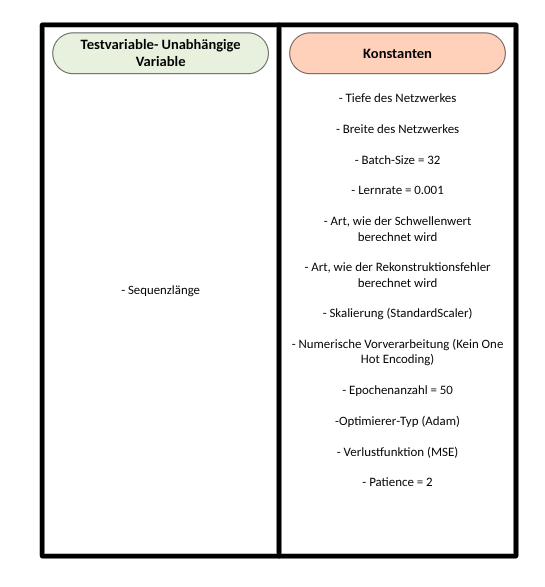
\includegraphics[width=0.7\linewidth]{Bilder/variablen}
		\caption{Überblick der Konstanten Werte und der unabhängigen Variable}
		\label{fig:variablen}
	\end{figure}

	Alle genannten Konstanten wie die Breite, Tiefe und Batch-Size bleiben dabei konstant. Weitere Faktoren wie die Berechnung des Rekonstruktionsfehlers, der Schwellenwert, die Skalierung (StandardScaler), die Anzahl von 50 der Trainings-Epochen, der Optimierer (Adam) und die Verlustfunktion (MSE) werden konstant gehalten, um einen fairen Vergleich der Modelle zu gewährleisten. Die gewählten Konstanten können zwar die erzielbaren Höchstwerte im Vergleich zu anderen Studien begrenzen, gewährleisten jedoch, dass die Analyse vergleichbar bleibt.
	\\[0.5em]
	Zusammenfassend ergibt sich, dass die Sequenzlänge als unabhängige Variable und die Metriken F1-Score, Balanced Accuracy sowie MCC als abhängige Variablen betrachtet werden.
	
	\section{Auswertung}
	\subsection{Berechnung der Mittelwerte}
	
	Um herauszufinden, wie hoch die Werte vom F1-Score, MCC und Balanced Accuracy haben sind, werden die Mittelwerte aller Runs je Sequenzlänge ausgerechnet.
	
	\begin{table}[H]
		\centering
		\caption{Vergleich der Modelle bei Sequenzlänge 25}
		\begin{tabular}{lcccc}
			\hline
			Modell & Sequenzlänge & F1-Score & MCC & Balanced Accuracy \\
			\hline
			IsolationForest & 25 & 0.7541 & 0.7587 & 0.8188 \\
			One-Class SVM & 25 & 0.7430 & 0.7411 & 0.8271 \\
			DBSCAN & 25 & 0.1928 & 0.3170 & 0.5538 \\
			\hline
		\end{tabular}
	\end{table}
	
	\begin{table}[H]
		\centering
		\caption{Übersicht der Ergebnisse für Sequenzlänge 45}
		\begin{tabular}{lcccc}
			\hline
			Modell & Sequenzlänge & F1-Score & MCC & Balanced Accuracy \\
			\hline
			IsolationForest & 45 & 0.6172 & 0.5904 & 0.7937 \\
			One-Class SVM & 45 & 0.6367 & 0.6185 & 0.7895 \\
			DBSCAN & 45 & 0.1237 & 0.2453 & 0.5332 \\
			\hline
		\end{tabular}
	\end{table}
	
	Es ist erkennbar, dass die Ergebnisse stark von der Sequenzlänge abhängen. Sequenzen der Länge 25 erzielen generell bessere Ergebnisse als Sequenzen der Länge 45, vermutlich weil kürzere Sequenzen für diese Modelle besser geeignet sind. In Zukunft sollte auch versucht werden, deutlich kürzere Sequenzen zu verwenden, zum Beispiel mit einer Länge von 1 bis 10. Dies könnte neue Erkenntnisse insbesondere bei kleinen Datensätzen liefern.
	\\[0.5em]
	DBSCAN erzielt unter allen Metriken und Sequenzlängen die niedrigsten Werte. Dies könnte auf die ungleiche Verteilung der Daten zurückzuführen sein. DBSCAN ist grundsätzlich ein Clustering-Verfahren – eine stark ungleiche Datenverteilung kann daher dazu führen, dass Anomalien falsch geclustert werden.
	\\[0.5em]
	OCSVM erreicht bei der Sequenzlänge 45 eine höhere MCC sowie einen höheren F1-Score. Isolation Forest erzielt hingegen bei der Sequenzlänge 25 bessere Werte in beiden Metriken sowie eine höhere Balanced Accuracy. OCSVM zeigt dafür bei der Sequenzlänge 25 eine höhere Balanced Accuracy als bei längeren Sequenzen.
	\\[0.5em]
	Die Mittelwerte zeigen klar, dass Sequenzlänge 25 für IF optimal ist, während OCSVM bei Sequenzlänge 45 besser abschneidet. Damit lässt sich die Hypothese aber weder verifizieren, noch falsifizieren.
	\\[0.5em]
	Wenn man alle Metriken zusammenrechnet, unabhängig von der Sequenzlänge erhält man ein anderes Bild:
	
	\begin{table}[H]
		\centering
		\caption{Übersicht der Ergebnisse}
		\begin{tabular}{lcccc}
			\hline
			Modell & Sequenzlänge & F1-Score & MCC & Balanced Accuracy \\
			\hline
			IsolationForest & 25 und 45 & 0.6857 & 0.6746 & 0.8063 \\
			One-Class SVM & 25 und 45 & 0.6899 & 0.6798 & 0.8083	  \\
			DBSCAN & 25 und 45 & 0.1583 & 0.2812 & 0,5435 \\
			\hline
		\end{tabular}
	\end{table}
	Bei der Summierung der Werte ergibt sich ein neues Bild: Unter allen Sequenzlängen erzielt OCSVM in allen drei Metriken die höchsten Ergebnisse, auch wenn sie nur knapp etwas höher sind als IF. Die Hypothese kann man hier schon als widerlegt ansehen, jedoch wäre dies vorurteilend. Unter anderem kann man hier bei der Berechnung der Mittelwerte zwar nur aussagen, wie "hoch" die Ergebnisse sind, aber nicht wie stabil sie sind. Es werden deshalb weitere Evaluierungsmetrikne benötigt, um ein genaues Bild davon zu bekommen, wie die Werte verteilt sind und wie sie zustande gekommen sind. 
	
	
	\subsubsection{Berechnung der Standardabweichung und Varianz}
	% --- Tabelle 1: Varianz, Seq. 25 ---
	\begin{table}[H]
		\centering
		\caption{Varianz der Modelle bei Sequenzlänge 25}
		\begin{tabular}{lccc}
			\hline
			Modell & F1-Score & MCC & BA \\
			\hline
			IF     & 0.000124 & 0.000220 & 0.000047 \\
			OCSVM  & 0.000568 & 0.000944 & 0.000087 \\
			DBSCAN & 0.003704 & 0.003892 & 0.000319 \\
			\hline
		\end{tabular}
	\end{table}
	
	% --- Tabelle 2: Varianz, Seq. 45 ---
	\begin{table}[H]
		\centering
		\caption{Varianz der Modelle bei Sequenzlänge 45}
		\begin{tabular}{lccc}
			\hline
			Modell & F1-Score & MCC & BA \\
			\hline
			IF     & 0.000318 & 0.000383 & 0.000073 \\
			OCSVM  & 0.000318 & 0.000382 & 0.000073 \\
			DBSCAN & 0.001706 & 0.002560 & 0.000130 \\
			\hline
		\end{tabular}
	\end{table}
	
	% --- Tabelle 3: Standardabweichung, Seq. 25 ---
	\begin{table}[H]
		\centering
		\caption{Standardabweichung der Modelle bei Sequenzlänge 25}
		\begin{tabular}{lccc}
			\hline
			Modell & F1-Score & MCC & BA \\
			\hline
			IF     & 0.01113 & 0.01484 & 0.00683 \\
			OCSVM  & 0.02382 & 0.03072 & 0.00933 \\
			DBSCAN & 0.06086 & 0.06239 & 0.01786 \\
			\hline
		\end{tabular}
	\end{table}
	
	% --- Tabelle 4: Standardabweichung, Seq. 45 ---
	\begin{table}[H]
		\centering
		\caption{Standardabweichung der Modelle bei Sequenzlänge 45}
		\begin{tabular}{lccc}
			\hline
			Modell & F1-Score & MCC & BA \\
			\hline
			IF     & 0.01783 & 0.01955 & 0.00857 \\
			OCSVM  & 0.01783 & 0.01955 & 0.00857 \\
			DBSCAN & 0.04131 & 0.05060 & 0.01138 \\
			\hline
		\end{tabular}
	\end{table}
	Zur Beurteilung der Stabilität der Modelle wurden die Varianz und Standardabweichung der F1-Score, Matthews Correlation Coefficient (MCC) und Balanced Accuracy (BA) über fünf Testläufe berechnet. Die Berechnungen erfolgten für Sequenzlängen von 25 und 45.
	\\[0.5em]
	Für Sequenzlänge 25 zeigt IF sehr geringe Varianzen und Standardabweichungen (F1-Score: Varianz $0.000124$, Std $0.0111$; MCC: Varianz $0.000220$, Std $0.0148$; BA: Varianz $0.000047$, Std $0.0068$). Auch bei längeren Sequenzen (45) bleibt die Streuung niedrig (F1-Score: Varianz $0.000318$, Std $0.0178$; MCC: Varianz $0.000382$, Std $0.0196$; BA: Varianz $0.000073$, Std $0.0086$). Dies zeigt, dass IF über die Testläufe hinweg sehr stabile Ergebnisse liefert.
	\\[0.5em]
	OCSVM zeigt bei Sequenzlänge 25 eine leicht höhere Streuung (F1-Score: Varianz $0.000568$, Std $0.0238$; MCC: Varianz $0.000944$, Std $0.0307$; BA: Varianz $0.000087$, Std $0.0093$), stabilisiert sich jedoch bei Sequenzlänge 45 (F1-Score: Varianz $0.000318$, Std $0.0178$; MCC: Varianz $0.000382$, Std $0.0196$; BA: Varianz $0.000073$, Std $0.0086$). Damit zeigt OCSVM eine gute Konsistenz, insbesondere bei längeren Sequenzen.
	\\[0.5em]
	DBSCAN weist im Vergleich zu IF und OCSVM deutlich höhere Varianz und Standardabweichung auf (z. B. F1-Score: Varianz $0.003704$, Std $0.0609$ bei Sequenzlänge 25; F1-Score: Varianz $0.001706$, Std $0.0413$ bei Sequenzlänge 45). Diese Werte deuten auf eine hohe Sensitivität gegenüber den Parametern und eine geringere Stabilität über die Testläufe hin.
	\\[0.5em]
	Kurz gesagt: IF ist über alle Testläufe am zuverlässigsten, OCSVM variiert ein wenig bei kurzen Sequenzen, DBSCAN ist am wenigsten zuverlässig. Hier zeigt sich, dass IF die stabilsten Werte also erzielte.
	
	\subsubsection{Friedman-Test}
	Der Friedman-Test\cite{Pereira2015} ist ein nicht-parametrischer Test, der prüft, ob es systematische Unterschiede zwischen mehreren verbundenen Gruppen gibt, z.B., ob verschiedene Modelle über mehrere Datensätze oder Sequenzlängen hinweg unterschiedliche Leistungen zeigen.
	\\[0.5em]
	Dabei liefert der Test zwei zentrale Kenngrößen: die Teststatistik Chi² und den p-Wert.
	\\[0.5em]
	Chi² ist die Teststatistik, die aus den Rängen der Beobachtungen berechnet wird und angibt, wie stark sich die Gruppen systematisch unterscheiden.
	\\[0.5em]
	Der p-Wert gibt an, wie wahrscheinlich es ist, dass die beobachteten Unterschiede zwischen den Gruppen zufällig entstanden sind. Ein kleiner p-Wert (z.B. größer als 0,05) deutet darauf hin, dass die Unterschiede statistisch signifikant sind.
	\\[0.5em]
	Für den Vergleich der Leistungsmetriken der drei Hybridmodelle über verschiedene Sequenzlängen wurde der Friedman-Test verwendet. In diesem Experiment entsprechen die verschiedenen Sequenzlängen den verbundenen Messungen, da jede Sequenzlänge für alle Modelle vorliegt.
	\\[0.5em]
	Ein weiterer Vorteil des Friedman-Tests ist, dass er keine Annahmen über die Normalverteilung der Daten macht. Parametrische Tests wie die ANOVA\footnote{\url{https://www.sciencedirect.com/science/article/abs/pii/0169743989800954}, letzter Zugriff am 28.August.2025} setzen voraus, dass die Messwerte innerhalb der Gruppen normalverteilt sind. Da dies bei den betrachteten Metriken (F1-Score, MCC, Balanced Accuracy) nicht garantiert werden kann, stellt der Friedman-Test eine robuste Alternative dar.
	\\[0.5em]
	Der Test basiert auf Rangplätzen innerhalb der Sequenzlängen und ist dadurch weniger anfällig für Ausreißer. Gleichzeitig liefert er einen p-Wert, der es erlaubt zu prüfen, ob mindestens ein Modell systematisch von den anderen abweicht. Somit eignet sich der Friedman-Test ideal, um die signifikanten Unterschiede in den Leistungsmetriken zwischen den Modellen nachzuweisen.
	\\[0.5em]
	
	Anbei sind die Ergebnisse des Tests:
	
	\begin{table}[H]
		\centering
		\caption{Friedman-Test Ergebnisse (seq. 25)}
		\begin{tabular}{lcccc}
			\toprule
			\textbf{Metrik} & \textbf{Chi²} & \textbf{p-Wert} & \textbf{Signifikanz} & \textbf{Seq.} \\
			\midrule
			F1-Score          & 10.000 & 0.0067 & Signifikante Unterschiede zwischen den Modellen & 25 \\
			MCC               &  8.400 & 0.0150 & Signifikante Unterschiede zwischen den Modellen & 25 \\
			Balanced Accuracy & 10.000 & 0.0067 & Signifikante Unterschiede zwischen den Modellen & 25 \\
			\bottomrule
		\end{tabular}
	\end{table}
	
	\begin{table}[H]
		\centering
		\caption{Friedman-Test Ergebnisse (seq. 45)}
		\begin{tabular}{lcccc}
			\toprule
			\textbf{Metrik} & \textbf{Chi²} & \textbf{p-Wert} & \textbf{Signifikanz} & \textbf{Seq.} \\
			\midrule
			F1-Score          & 10.000 & 0.0067 & Signifikante Unterschiede zwischen den Modellen & 45 \\
			MCC               & 10.000 & 0.0067 & Signifikante Unterschiede zwischen den Modellen & 45 \\
			Balanced Accuracy & 10.000 & 0.0067 & Signifikante Unterschiede zwischen den Modellen & 45 \\
			\bottomrule
		\end{tabular}
	\end{table}
	Da die p-Werte alle unter 0.05 liegen, ist es sehr unwahrscheinlich, dass die beobachteten Unterschiede zufällig entstanden sind. Die Chi²-Werte sind größer als 0, was zusätzlich auf Abweichungen von der Nullhypothese hinweist. Somit wird die Nullhypothese abgelehnt.
	\\[0.5em]
	Wichtig ist zu beachten, dass der Friedman-Test nur eine abhängige Variable untersucht, weshalb für jede Metrik ein separater Test durchgeführt wurde. Er stellt also nicht den gesamten Zusammenhang zwischen den einzelnen Metriken dar, sondern die signifikanten Unterschiede einer Metrik je Modell. 
	\\[0.5em]
	Dies ist gerechtfertigt, da die Stichprobengröße pro Modell klein ist und keine Normalverteilung der Metriken vorausgesetzt wird. Eine multivariate Analyse über alle Metriken hinweg könnte theoretisch Korrelationsstrukturen berücksichtigen, ist jedoch aufgrund der geringen Stichprobengröße hier nicht sinnvoll. Die Stichprobe wurde bewusst klein gehalten, da bereits erste Tests zeigten, dass bei sehr hohen Sequenzlängen die Modellgüte in allen Metriken deutlich abnimmt. Ziel war es daher, den Einfluss unterschiedlicher Fenstergrößen gezielt zu analysieren, ohne den Rahmen der Arbeit zu sprengen. Mit den beiden gewählten Sequenzlängen (25 und 45) lässt sich die Diskrepanz zwischen kürzeren und längeren Kontexten ausreichend abbilden und validieren. Ein Vergleich mit zwei Sequenzlängen ist für die Fragestellung dieser Arbeit daher angemessen. In zukünftigen Arbeiten ist ein Vergleich mit mehreren Sequenzlängen wie erwähnt von Bedeutung.
	\\[0.5em]
	Um zudem noch zu zeigen welche Modelle genau nun sich gering unterscheiden ist ein sogenannter Post-Hoc-Test notwendig.
	
	\subsubsection{Nemenyi-Test}
	Der Nemenyi-Test ist ein nichtparametrischer Post-hoc-Test\footnote{Ein post-hoc-Test ist ein statistisches Verfahren, das nach einem Test durchgeführt wird, um genau zu bestimmen, welche Gruppen sich signifikant voneinander unterscheiden.}, der nach einem Friedman-Test angewendet wird, wenn signifikante Unterschiede zwischen mehreren verbundenen Gruppen festgestellt wurden. Er dient dazu, paarweise Vergleiche zwischen den Gruppen durchzuführen und zu prüfen, welche Paare sich statistisch signifikant unterscheiden.
	\\[0.5em]
	Im Gegensatz zu parametrischen Tests setzt der Nemenyi-Test keine Normalverteilung der Daten voraus, sondern arbeitet auf den Rängen der Beobachtungen. Die Ergebnisse werden in einer Matrix von p-Werten dargestellt, die für jedes Gruppenpaar angibt, ob der Unterschied signifikant ist.
	\\[0.5em]
	In diesem Fall wurden drei Hybridmodelle hinsichtlich verschiedener Leistungsmetriken (F1-Score, MCC, Balanced Accuracy) bewertet. Da die Modelle auf denselben Datensätzen getestet wurden, handelt es sich um verbundene (abhängige) Stichproben, und die Daten sind nicht notwendigerweise normalverteilt. Nach dem Friedman-Test, der einen globalen Unterschied zwischen den Modellen zeigte, eignet sich der Nemenyi-Test ideal, um konkret zu bestimmen, welche Modellpaare sich signifikant unterscheiden.
	
	\begin{table}[H]
		\centering
		\caption{Nemenyi Post-hoc Test: F1-Score, Sequenzlänge 25}
		\begin{tabular}{lccc}
			\hline
			& IF & OCSVM & DBSCAN \\
			\hline
			IF      & 1.0000 & 0.2538 & 0.0045 \\
			OCSVM   & 0.2538 & 1.0000 & 0.2538 \\
			DBSCAN  & 0.0045 & 0.2538 & 1.0000 \\
			\hline
		\end{tabular}
	\end{table}
	
	\begin{table}[H]
		\centering
		\caption{Nemenyi Post-hoc Test: MCC, Sequenzlänge 25}
		\begin{tabular}{lccc}
			\hline
			& IF & OCSVM & DBSCAN \\
			\hline
			IF      & 1.0000 & 0.6094 & 0.0123 \\
			OCSVM   & 0.6094 & 1.0000 & 0.1394 \\
			DBSCAN  & 0.0123 & 0.1394 & 1.0000 \\
			\hline
		\end{tabular}
	\end{table}
	
	\begin{table}[H]
		\centering
		\caption{Nemenyi Post-hoc Test: Balanced Accuracy, Sequenzlänge 25}
		\begin{tabular}{lccc}
			\hline
			& IF & OCSVM & DBSCAN \\
			\hline
			IF      & 1.0000 & 0.2538 & 0.2538 \\
			OCSVM   & 0.2538 & 1.0000 & 0.0045 \\
			DBSCAN  & 0.2538 & 0.0045 & 1.0000 \\
			\hline
		\end{tabular}
	\end{table}
	
	\begin{table}[H]
		\centering
		\caption{Nemenyi Post-hoc Test: F1-Score, Sequenzlänge 45}
		\begin{tabular}{lccc}
			\hline
			& IF & OCSVM & DBSCAN \\
			\hline
			IF      & 1.0000 & 1.0000 & 0.0466 \\
			OCSVM   & 1.0000 & 1.0000 & 0.0466 \\
			DBSCAN  & 0.0466 & 0.0466 & 1.0000 \\
			\hline
		\end{tabular}
	\end{table}
	
	\begin{table}[H]
		\centering
		\caption{Nemenyi Post-hoc Test: MCC, Sequenzlänge 45}
		\begin{tabular}{lccc}
			\hline
			& IF & OCSVM & DBSCAN \\
			\hline
			IF      & 1.0000 & 1.0000 & 0.0466 \\
			OCSVM   & 1.0000 & 1.0000 & 0.0466 \\
			DBSCAN  & 0.0466 & 0.0466 & 1.0000 \\
			\hline
		\end{tabular}
	\end{table}
	
	\begin{table}[H]
		\centering
		\caption{Nemenyi Post-hoc Test: Balanced Accuracy, Sequenzlänge 45}
		\begin{tabular}{lccc}
			\hline
			& IF & OCSVM & DBSCAN \\
			\hline
			IF      & 1.0000 & 1.0000 & 0.0466 \\
			OCSVM   & 1.0000 & 1.0000 & 0.0466 \\
			DBSCAN  & 0.0466 & 0.0466 & 1.0000 \\
			\hline
		\end{tabular}
	\end{table}
	Die Nemenyi-Post-hoc-Tests wurden durchgeführt, um nach den signifikanten Ergebnissen des Friedman-Tests die paarweisen Unterschiede zwischen den drei Modellen (IF, OCSVM, DBSCAN) für jede Metrik und Sequenzlänge zu identifizieren.
	\\[0.5em]
	Für Sequenzlänge 25 zeigt der F1-Score, dass IF und OCSVM keinen signifikanten Unterschied aufweisen (p = 0.2538) und somit ähnlich performen, während IF im Vergleich zu DBSCAN signifikant besser ist (p = 0.0045) und OCSVM vs DBSCAN keinen signifikanten Unterschied zeigt (p = 0.2538). 
	\\[0.5em]
	Beim MCC unterscheiden sich IF und OCSVM nicht signifikant (p = 0.6094), IF ist jedoch signifikant besser als DBSCAN (p = 0.0123), während OCSVM vs DBSCAN keinen signifikanten Unterschied zeigt (p = 0.1394). Bei der Balanced Accuracy zeigen IF vs OCSVM (p = 0.2538) und IF vs DBSCAN (p = 0.2538) keine signifikanten Unterschiede, während OCSVM vs DBSCAN signifikant ist (p = 0.0045), wobei OCSVM besser abschneidet und IF im Mittelfeld liegt.
	\\[0.5em]
	Für Sequenzlänge 45 zeigt der F1-Score, dass IF und OCSVM keinen signifikanten Unterschied aufweisen (p = 1.000), während sowohl IF vs DBSCAN als auch OCSVM vs DBSCAN signifikant sind (p = 0.0466), wodurch DBSCAN deutlich schlechter performt und IF und OCSVM vergleichbar bleiben. 
	\\[0.5em]
	Beim MCC zeigt sich dasselbe Muster: DBSCAN unterscheidet sich signifikant von IF und OCSVM (p = 0.0466), IF und OCSVM unterscheiden sich nicht (p = 1.000), DBSCAN ist also auch im MCC schwächer. Bei der Balanced Accuracy gilt dasselbe: DBSCAN zeigt signifikant niedrigere Werte als IF und OCSVM (p = 0.0466), IF und OCSVM unterscheiden sich nicht (p = 1.000). 
	\\[0.5em]
	Insgesamt zeigt die Post-hoc-Analyse, dass insbesondere DBSCAN im Vergleich zu IF und OCSVM deutlich schlechter abschneidet, während IF und OCSVM weitgehend vergleichbar sind, was die globalen Unterschiede bestätigt, die bereits im Friedman-Test festgestellt wurden.
	\\[0.5em]
	Somit wird die Nullhypothese, dass alle Modelle gleich gut sind, verworfen, und die Unterschiede zwischen den Modellen sind statistisch signifikant und nicht zufällig entstanden.
	
	\section{Diskussion}
	Die Ergebnisse zeigen deutliche Unterschiede in der Klassifikationsleistung zwischen den getesteten Verfahren und den Sequenzlängen. Die Tests für die Sequenzlängen 25 und 45 verdeutlichen, dass insbesondere Isolation Forest (IF) und One-Class SVM (OCSVM) insgesamt gute Ergebnisse liefern, während DBSCAN deutlich schlechter abschneidet (s. Tabellen und Post-hoc-Analyse).
	\\[0.5em]
	IF und OCSVM erreichen konstant hohe Werte in F1-Score, MCC und Balanced Accuracy. Das bedeutet, dass die Modelle die meisten Anomalien korrekt erkennen, gleichzeitig aber nur wenige normale Logs fälschlicherweise als anomal klassifizieren. DBSCAN weist dagegen deutlich niedrigere Werte auf und ist instabiler über die Testläufe.
	\\[0.5em]
	Für OCSVM zeigt sich, dass die Leistung bei längeren Sequenzen (45) leicht besser in F1 und MCC ist, während IF bei kürzeren Sequenzen (25) besonders stabile Ergebnisse liefert. DBSCAN bleibt unabhängig von der Sequenzlänge deutlich schlechter, was mit seiner Sensitivität gegenüber Parameterwahl und ungleich verteilten Daten zusammenhängt.  
	\\[0.5em]
	Weitere Einflussfaktoren auf die Ergebnisse könnten darin liegen, dass die Tiefe und Breite der LSTM-Autoencoder-Komponente möglicherweise zu gering oder zu hoch für die datenhungrigen Hybridmodelle war und das Training nur über 50 Epochen unter Einsatz von EarlyStopping erfolgte.  
	\\[0.5em]
	Dies deutet darauf hin, dass der LSTM-Autoencoder die auffälligsten Muster normaler Logs sehr schnell gelernt hat. Gleichzeitig bedeutet dies, dass die Modelle möglicherweise nicht alle Feinheiten der normalen Daten erfasst haben und daher empfindlicher gegenüber kleinen Variationen oder Anomalien in den Testdaten sind. Das frühe Stoppen verhindert extremes Overfitting, kann aber dazu führen, dass die Rekonstruktion subtiler normaler Muster unvollständig bleibt.  
	\\[0.5em]
	Außerdem wurde das Verhältnis der Features nur unzureichend berücksichtigt. Die abhängige Variable stellt zwar das Label dar, das den Log als anomal oder normal klassifiziert, jedoch wurden IP-Adressen und Features wie Standort und Zeit entfernt. Die Angriffsszenarien mussten daher innerhalb normaler Zeiträume, beispielsweise mittags, stattfinden, um die Fähigkeiten des LSTM-Autoencoders wirklich zu testen. Einflussreicher sind nun Features wie Name, Eventtyp und andere Faktoren. Die Frage, in welchem Ausmaß einzelne Features die Klassifikation beeinflussen, bleibt Gegenstand zukünftiger Arbeiten.  
	\\[0.5em]
	Die Modelle wurden auf einer CPU trainiert, da keine GPU verfügbar war. Aufgrund der begrenzten Rechenressourcen könnten sich Trainingsdauer, Batch-Größe und numerische Präzision auf Modellstabilität und Varianz der Ergebnisse ausgewirkt haben.  
	\\[0.5em]
	% Ein weiteres Problem, das im Kontext des maschinellen Lernens beachtet werden sollte, ist die eingeschränkte Reproduzierbarkeit mancher Tests. Wie zuvor erwähnt, kann die Wahl der Dropout-Rate die Reliabilität der Ergebnisse beeinflussen, wenn auch nur in geringem Maße. In anderen Versuchen könnte das Verfahren Isolation Forest daher in bestimmten Bereichen zu besseren Resultaten führen. Dieses Problem der eingeschränkten Reproduzierbarkeit ist in der Forschung nach wie vor nicht vollständig gelöst. Auch wenn Dropout nicht deterministisch ist, zeigen Reimers und Gurevych \cite{reimers2017score}, dass der gewählte Seed keinen dominanten Einflussfaktor für die Reproduzierbarkeit darstellt und dass mehrere unabhängige Testläufe aussagekräftiger sind als die bloße Festlegung eines deterministischen Startwertes. Zudem wird Variabilität in dieser Arbeit so gewährleistet.
	\\[0.5em]
	Ein weiterer Grund für die beobachteten Unterschiede ist, dass OCSVM sich besonders für kleinere Datensätze eignet, während IF tendenziell bei größeren Datenmengen stärker performt. Die 39.000 Logs waren für OCSVM ausreichend, während IF bei noch größeren Datensätzen potenziell höhere Werte erzielen könnte.
	\\[0.5em]
	Nach allen metrischen Messungen lässt sich die Hypothese nur im Vergleich zu DBSCAN verifizieren; gegenüber OCSVM hingegen nicht. Somit ist die Hypothese in dieser Arbeit weder vollständig verifizierbar noch falsifizierbar. Änderungen an Parametern, Regularisierungstechniken oder der Trainingskonfiguration könnten zu anderen Ergebnissen führen. Die Resultate hängen stark von Faktoren wie den Hyperparametern, dem Datensatz und der verfügbaren Rechenleistung ab. Unter anderen Bedingungen könnten daher abweichende Ergebnisse erzielt werden. Weitere Studien mit einem alternativen Testsetup, anderen Modellarchitekturen oder zusätzlichen Daten könnten dazu beitragen, die Aussagekraft für diesen Fall zu erhöhen.
	
	\section{Fazit}
	Insgesamt zeigen die Ergebnisse, dass Hybridmodelle in der Lage sind, Anomalien in Keycloak-Logs zuverlässig zu erkennen. Dabei spielen sowohl die Architektur des LSTM-Autoencoders als auch die gewählte Sequenzlänge eine entscheidende Rolle für die Erkennungsleistung, insbesondere angesichts des stark unbalancierten Datensatzes.
	\\[0.5em]
	Die Methodik stellt sicher, dass sensible Unternehmensdaten nicht verwendet werden: Die Trainings- und Testdaten basieren auf generierten Logs, während durch Selenium-basierte Tests und die Keycloak-API authentische Log-Muster abgebildet werden. Insgesamt unterstreichen die Ergebnisse das Potenzial von LSTM-Autoencodern in Kombination mit klassischen Anomalieerkennungsverfahren für die automatisierte Überwachung von Keycloak-Logs und demonstrieren, dass die Wahl der Modellkombination und der Hyperparameter maßgeblich für die Performance ist.
	\\[0.5em]
	Die Ergebnisse haben gezeigt, dass die Verifizierung der Hypothese stark von der Wahl der Parameter der LSTM-AE-Architektur, der Größe des Datensatzes und von der Rechenleistung der Grafikkarte abhängig ist, sowie der Verteilung und Anzahl der Anomalien im Datensatz.
	\\[0.5em]
	Für weitere Studien ist es wichtig, andere unabhängige Variablen oder auch mehreren wie mehreren Datensätzen zu achten, sowie eventuell andere Metriken mehr mit einzubeziehen, wie bspw. die AUC-PR-Werte.
		
	\section{Ausblick}
	\subsection{Wirtschaftliche Anwendung}
	Das Unternehmen intension kann mit weiteren Tests in naher Zukunft und mit mehr Forschung ein Anomalieerkennungstool entwickeln. Mit zusätzlichen kombinierten Produkten wie z.B. ELK\footnote{Definition von ELK: \url{https://www.elastic.co/elastic-stack/},letzter Zugriff am 28.August.2025} könnte das Anomalieerkennungstool Insider-Angriffe, Intrusionsangriffe und generelle Anomalien erkennen. Es ist wichtig, dass das Produkt richtig integriert wird und getestet wird, welche Schnittstellen mit welchen Produkten integrierbar sind. Dies erfordert jedoch weiterhin Zeit, Forschung und ein größeres Team, um eine professionelle Umsetzung zu gewährleisten.
	
	\subsection{Wissenschaftlicher Ausblick}
	In Zukunft könnten weitere Algorithmen oder alternative Architekturen in die Untersuchung aufgenommen werden. Mit einer größeren Menge an Trainings- und Testdaten ließe sich die Architektur weiter optimieren und generalisieren. Auf Basis der gewonnenen Erkenntnisse wäre zudem die Entwicklung eines praxistauglichen Anomalieerkennungstools denkbar. Die konkrete Leistungsfähigkeit hängt jedoch stark vom jeweiligen Testszenario ab.
	In dieser Arbeit wurden rund 39.000 Log-Einträge verwendet, wobei zwei feste Sequenzlängen und eine spezifische Architektur untersucht wurden. Unter anderen Bedingungen könnten die Erkennungsergebnisse deutlich abweichen. So könnte beispielsweise ein LSTM-Autoencoder kombiniert mit Isolation Forest in einem anderen Szenario bessere Resultate erzielen als OCSVM oder DBSCAN.
	Daher erscheint es sinnvoll, weitere Tests mit komplexeren Angriffsszenarien, zusätzlichen Trainingsdaten und alternativen Methoden zur Schwellenwertbestimmung durchzuführen.
	
	\subsection{Angriffe}
	Die hier verwendeten Angriffsszenarien waren vergleichsweise einfach gehalten. Angriffe über Drittanbieter im SSO (z.B. eine Attacke auf ein Google-Konto mit anschließendem Zugriff auf Keycloak) oder über das Netzwerk wurden nicht berücksichtigt. Auch Szenarien wie Zertifikatsfälschungen in Keycloak sollten in zukünftigen Studien einbezogen werden. Durch die Einbeziehung realistischerer und variablerer Angriffsmuster könnten die Modelle lernen, mit komplexeren Angriffen umzugehen.
	
\newpage
\bibliography{quellen} 
\newpage 
\renewcommand{\notesname}{Fußnotenverzeichnis}
\renewcommand{\enoteformat}{\rightskip0pt\leftskip0pt\vspace{0.5em}\noindent\makebox[2em][l]{\theenmark}}
\theendnotes
\newpage

\section*{Anhang}
\subsection*{Ergebnisse mit der Sequenzlänge 25}
\subsubsection{Sequenzlänge 25, Testlauf 1}
\begin{table}[H]
	\centering
	\caption{Ergebnisse von LSTM-AE-IF (Sequenzlänge 25, Testlauf 1)}
	\begin{tabular}{lcc}
		\hline
		Metrik & Wert \\
		\hline
		Best Threshold by F1 & -0.1938 \\
		Precision & 0.9461 \\
		Recall & 0.6345 \\
		F1-Score & 0.7596 \\
		ROC-AUC & 0.9295 \\
		AUC-PR & 0.6159 \\
		Matthews Correlation Coefficient (MCC) & 0.7673 \\
		Balanced Accuracy & 0.8165 \\
		Accuracy & 0.9829 \\
		\hline
	\end{tabular}
\end{table}

\begin{table}[H]
	\centering
	\caption{Ergebnisse von LSTM-AE-OCSVM (Sequenzlänge 25, Testlauf 1)}
	\begin{tabular}{lcc}
		\hline
		Metrik & Wert \\
		\hline
		Best Threshold by F1 & -0.0033 \\
		Precision & 0.8956 \\
		Recall & 0.6546 \\
		F1-Score & 0.7564 \\
		ROC-AUC & 0.7532 \\
		AUC-PR & 0.6010 \\
		Matthews Correlation Coefficient (MCC) & 0.7572 \\
		Balanced Accuracy & 0.8256 \\
		Accuracy & 0.9821 \\
		\hline
	\end{tabular}
\end{table}

\begin{table}[H]
	\centering
	\caption{Ergebnisse von LSTM-AE-DBSCAN(Sequenzlänge 25, Testlauf 1)}
	\begin{tabular}{lcc}
		\hline
		Metrik & Wert \\
		\hline
		Passender eps-Wert & 0.07 \\
		Anomalien & 32 \\
		Precision & 1.0000 \\
		Recall & 0.1285 \\
		F1-Score & 0.2278 \\
		Matthews Correlation Coefficient (MCC) & 0.3517 \\
		Balanced Accuracy & 0.5643 \\
		ROC-AUC & 0.5643 \\
		AUC-PR & 0.1656 \\
		Accuracy & 0.9630 \\
		\hline
	\end{tabular}
\end{table}

\subsubsection{Sequenzlänge 25, Testlauf 2}
\begin{table}[H]
	\centering
	\caption{Ergebnisse von LSTM-AE-IF (Sequenzlänge 25, Testlauf 2)}
	\begin{tabular}{lcc}
		\hline
		Metrik & Wert \\
		\hline
		Best Threshold by F1 & -0.1885 \\
		Precision & 0.9689 \\
		Recall & 0.6265 \\
		F1-Score & 0.7610 \\
		ROC-AUC & 0.9391 \\
		AUC-PR & 0.6229 \\
		Matthews Correlation Coefficient (MCC) & 0.7720 \\
		Balanced Accuracy & 0.8128 \\
		Accuracy & 0.9833 \\
		\hline
	\end{tabular}
\end{table}

\begin{table}[H]
	\centering
	\caption{Ergebnisse von LSTM-AE-OCSVM (Sequenzlänge 25, Testlauf 2)}
	\begin{tabular}{lcc}
		\hline
		Metrik & Wert \\
		\hline
		Best Threshold by F1 & -0.0023 \\
		Precision & 0.9573 \\
		Recall & 0.6305 \\
		F1-Score & 0.7603 \\
		ROC-AUC & 0.7528 \\
		AUC-PR & 0.6193 \\
		Matthews Correlation Coefficient (MCC) & 0.7696 \\
		Balanced Accuracy & 0.8146 \\
		Accuracy & 0.9831 \\
		\hline
	\end{tabular}
\end{table}

\begin{table}[H]
	\centering
	\caption{Ergebnisse von LSTM-AE-DBSCAN (Sequenzlänge 25, Testlauf 2)}
	\begin{tabular}{lcc}
		\hline
		Metrik & Wert \\
		\hline
		Passender eps-Wert & 0.08 \\
		Anomalien & 31 \\
		Precision & 1.0000 \\
		Recall & 0.1245 \\
		F1-Score & 0.2214 \\
		Matthews Correlation Coefficient (MCC) & 0.3462 \\
		Balanced Accuracy & 0.5622 \\
		ROC-AUC & 0.5622 \\
		AUC-PR & 0.1617 \\
		Accuracy & 0.9628 \\
		\hline
	\end{tabular}
\end{table}

\subsubsection{Sequenzlänge 25, Testlauf 3}
\begin{table}[H]
	\centering
	\caption{Ergebnisse von LSTM-AE-IF (Sequenzlänge 25, Testlauf 3)}
	\begin{tabular}{lcc}
		\hline
		Metrik & Wert \\
		\hline
		Best Threshold by F1 & -0.1852 \\
		Precision & 0.8564 \\
		Recall & 0.6466 \\
		F1-Score & 0.7368 \\
		ROC-AUC & 0.9315 \\
		AUC-PR & 0.5688 \\
		Matthews Correlation Coefficient (MCC) & 0.7346 \\
		Balanced Accuracy & 0.8209 \\
		Accuracy & 0.9804 \\
		\hline
	\end{tabular}
\end{table}

\begin{table}[H]
	\centering
	\caption{Ergebnisse von LSTM-AE-OCSVM (Sequenzlänge 25, Testlauf 3)}
	\begin{tabular}{lcc}
		\hline
		Metrik & Wert \\
		\hline
		Best Threshold by F1 & -0.0036 \\
		Precision & 0.8482 \\
		Recall & 0.6506 \\
		F1-Score & 0.7364 \\
		ROC-AUC & 0.7511 \\
		AUC-PR & 0.5667 \\
		Matthews Correlation Coefficient (MCC) & 0.7332 \\
		Balanced Accuracy & 0.8227 \\
		Accuracy & 0.9802 \\
		\hline
	\end{tabular}
\end{table}

\begin{table}[H]
	\centering
	\caption{Ergebnisse von LSTM-AE-DBSCAN (Sequenzlänge 25, Testlauf 3)}
	\begin{tabular}{lcc}
		\hline
		Metrik & Wert \\
		\hline
		Precision & 1.0000 \\
		Recall & 0.0442 \\
		F1-Score & 0.0846 \\
		Matthews Correlation Coefficient (MCC) & 0.2059 \\
		Balanced Accuracy & 0.5221 \\
		ROC-AUC & 0.5221 \\
		AUC-PR & 0.0848 \\
		Accuracy & 0.9594 \\
		\hline
	\end{tabular}
\end{table}


\subsubsection{Sequenzlänge 25, Testlauf 4}
\begin{table}[H]
	\centering
	\caption{Ergebnisse von LSTM-AE-IF (Sequenzlänge 25, Testlauf 4)}
	\begin{tabular}{lcc}
		\hline
		Metrik & Wert \\
		\hline
		Best Threshold by F1 & -0.1754 \\
		Precision & 0.9235 \\
		Recall & 0.6305 \\
		F1-Score & 0.7494 \\
		ROC-AUC & 0.9323 \\
		AUC-PR & 0.5980 \\
		Matthews Correlation Coefficient (MCC) & 0.7550 \\
		Balanced Accuracy & 0.8141 \\
		Accuracy & 0.9821 \\
		\hline
	\end{tabular}
\end{table}

\begin{table}[H]
	\centering
	\caption{Ergebnisse von LSTM-AE-OCSVM (Sequenzlänge 25, Testlauf 4)}
	\begin{tabular}{lcc}
		\hline
		Metrik & Wert \\
		\hline
		Best Threshold by F1 & -0.0025 \\
		Precision & 0.7265 \\
		Recall & 0.6827 \\
		F1-Score & 0.7039 \\
		ROC-AUC & 0.7498 \\
		AUC-PR & 0.5095 \\
		Matthews Correlation Coefficient (MCC) & 0.6916 \\
		Balanced Accuracy & 0.8357 \\
		Accuracy & 0.9756 \\
		\hline
	\end{tabular}
\end{table}

\begin{table}[H]
	\centering
	\caption{Ergebnisse von LSTM-AE-DBSCAN (Sequenzlänge 25, Testlauf 4)}
	\begin{tabular}{lcc}
		\hline
		Metrik & Wert \\
		\hline
		Passender eps-Wert & 0.06 \\
		Anomalien & 31 \\
		Precision & 1.0000 \\
		Recall & 0.1245 \\
		F1-Score & 0.2214 \\
		Matthews Correlation Coefficient (MCC) & 0.3462 \\
		Balanced Accuracy & 0.5622 \\
		ROC-AUC & 0.5622 \\
		AUC-PR & 0.1617 \\
		Accuracy & 0.9628 \\
		\hline
	\end{tabular}
\end{table}

\subsubsection{Sequenzlänge 25, Testlauf 5}
\begin{table}[H]
	\centering
	\caption{Ergebnisse von LSTM-AE-IF (Sequenzlänge 25, Testlauf 5)}
	\begin{tabular}{lcc}
		\hline
		Metrik & Wert \\
		\hline
		Best Threshold by F1 & -0.2036 \\
		Precision & 0.9016 \\
		Recall & 0.6627 \\
		F1-Score & 0.7639 \\
		ROC-AUC & 0.9354 \\
		AUC-PR & 0.6118 \\
		Matthews Correlation Coefficient (MCC) & 0.7647 \\
		Balanced Accuracy & 0.8297 \\
		Accuracy & 0.9826 \\
		\hline
	\end{tabular}
\end{table}

\begin{table}[H]
	\centering
	\caption{Ergebnisse von LSTM-AE-OCSVM (Sequenzlänge 25, Testlauf 5)}
	\begin{tabular}{lcc}
		\hline
		Metrik & Wert \\
		\hline
		Best Threshold by F1 & -0.0030 \\
		Precision & 0.8579 \\
		Recall & 0.6787 \\
		F1-Score & 0.7578 \\
		ROC-AUC & 0.7523 \\
		AUC-PR & 0.5959 \\
		Matthews Correlation Coefficient (MCC) & 0.7540 \\
		Balanced Accuracy & 0.8369 \\
		Accuracy & 0.9816 \\
		\hline
	\end{tabular}
\end{table}

\begin{table}[H]
	\centering
	\caption{Ergebnisse von LSTM-AE-DBSCAN (Sequenzlänge 25, Testlauf 5)}
	\begin{tabular}{lcc}
		\hline
		Metrik & Wert \\
		\hline
		Passender eps-Wert & 0.07 \\
		Anomalien & 29 \\
		Precision & 1.0000 \\
		Recall & 0.1165 \\
		F1-Score & 0.2086 \\
		Matthews Correlation Coefficient (MCC) & 0.3348 \\
		Balanced Accuracy & 0.5582 \\
		ROC-AUC & 0.5582 \\
		AUC-PR & 0.1540 \\
		Accuracy & 0.9624 \\
		\hline
	\end{tabular}
\end{table}
\newpage
\subsection*{Ergebnisse mit der Sequenzlänge 45}
\subsubsection{Sequenzlänge 25, Testlauf 1}
\begin{table}[H]
	\centering
	\caption{Ergebnisse von LSTM-AE-IF (Sequenzlänge 45, Testlauf 1)}
	\begin{tabular}{lc}
		\hline
		Metrik & Wert \\
		\hline
		Best Threshold by F1 & -0.2616 \\
		Precision & 0.6174 \\
		Recall & 0.6015 \\
		F1-Score & 0.6094 \\
		ROC-AUC & 0.7344 \\
		AUC-PR & 0.3980 \\
		Matthews Correlation Coefficient (MCC) & 0.5819 \\
		Balanced Accuracy & 0.7875 \\
		Accuracy & 0.9486 \\
		\hline
	\end{tabular}
\end{table}

\begin{table}[H]
	\centering
	\caption{Ergebnisse von LSTM-AE-OCSVM (Sequenzlänge 45, Testlauf 1)}
	\begin{tabular}{lc}
		\hline
		Metrik & Wert \\
		\hline
		Best Threshold by F1 & -0.0214 \\
		Precision & 0.6786 \\
		Recall & 0.6350 \\
		F1-Score & 0.6560 \\
		ROC-AUC & 0.6910 \\
		AUC-PR & 0.4552 \\
		Matthews Correlation Coefficient (MCC) & 0.6328 \\
		Balanced Accuracy & 0.8067 \\
		Accuracy & 0.9556 \\
		\hline
	\end{tabular}
\end{table}

\begin{table}[H]
	\centering
	\caption{Ergebnisse von LSTM-AE-DBSCAN (Sequenzlänge 45, Testlauf 1)}
	\begin{tabular}{lc}
		\hline
		Metrik & Wert \\
		\hline
		Passender eps-Wert & 0.04 \\
		Anomalien & 29 \\
		Precision & 1.0000 \\
		Recall & 0.0746 \\
		F1-Score & 0.1388 \\
		Matthews Correlation Coefficient (MCC) & 0.2644 \\
		Balanced Accuracy & 0.5373 \\
		ROC-AUC & 0.5373 \\
		AUC-PR & 0.1362 \\
		Accuracy & 0.9383 \\
		\hline
	\end{tabular}
\end{table}


\subsubsection{Sequenzlänge 25, Testlauf 2}
\begin{table}[H]
	\centering
	\caption{Ergebnisse von LSTM-AE-IF (Sequenzlänge 45, Testlauf 2)}
	\begin{tabular}{lc}
		\hline
		Metrik & Wert \\
		\hline
		Best Threshold by F1 & -0.2639 \\
		Precision & 0.6489 \\
		Recall & 0.6272 \\
		F1-Score & 0.6379 \\
		ROC-AUC & 0.8038 \\
		AUC-PR & 0.4319 \\
		Matthews Correlation Coefficient (MCC) & 0.6126 \\
		Balanced Accuracy & 0.8015 \\
		Accuracy & 0.9525 \\
		\hline
	\end{tabular}
\end{table}

\begin{table}[H]
	\centering
	\caption{Ergebnisse von LSTM-AE-OCSVM (Sequenzlänge 45, Testlauf 2)}
	\begin{tabular}{lc}
		\hline
		Metrik & Wert \\
		\hline
		Best Threshold by F1 & -0.0234 \\
		Precision & 0.6464 \\
		Recall & 0.6298 \\
		F1-Score & 0.6380 \\
		ROC-AUC & 0.6873 \\
		AUC-PR & 0.4318 \\
		Matthews Correlation Coefficient (MCC) & 0.6126 \\
		Balanced Accuracy & 0.8026 \\
		Accuracy & 0.9524 \\
		\hline
	\end{tabular}
\end{table}

\begin{table}[H]
	\centering
	\caption{Ergebnisse von LSTM-AE-DBSCAN (Sequenzlänge 45, Testlauf 2)}
	\begin{tabular}{lc}
		\hline
		Metrik & Wert \\
		\hline
		Precision & 1.0000 \\
		Recall & 0.0257 \\
		F1-Score & 0.0501 \\
		Matthews Correlation Coefficient (MCC) & 0.1550 \\
		Balanced Accuracy & 0.5129 \\
		ROC-AUC & 0.5129 \\
		AUC-PR & 0.0906 \\
		Accuracy & 0.9351 \\
		\hline
	\end{tabular}
\end{table}


\subsubsection{Sequenzlänge 25, Testlauf 3}
\begin{table}[H]
	\centering
	\caption{Ergebnisse von LSTM-AE-IF (Sequenzlänge 45, Testlauf 3)}
	\begin{tabular}{lc}
		\hline
		Metrik & Wert \\
		\hline
		Best Threshold by F1 & -0.2698 \\
		Precision & 0.6305 \\
		Recall & 0.6272 \\
		F1-Score & 0.6289 \\
		ROC-AUC & 0.8627 \\
		AUC-PR & 0.4203 \\
		Matthews Correlation Coefficient (MCC) & 0.6024 \\
		Balanced Accuracy & 0.8005 \\
		Accuracy & 0.9507 \\
		\hline
	\end{tabular}
\end{table}

\begin{table}[H]
	\centering
	\caption{Ergebnisse von LSTM-AE-OCSVM (Sequenzlänge 45, Testlauf 3)}
	\begin{tabular}{lc}
		\hline
		Metrik & Wert \\
		\hline
		Best Threshold by F1 & -0.0147 \\
		Precision & 0.6604 \\
		Recall & 0.6350 \\
		F1-Score & 0.6474 \\
		ROC-AUC & 0.6867 \\
		AUC-PR & 0.4437 \\
		Matthews Correlation Coefficient (MCC) & 0.6229 \\
		Balanced Accuracy & 0.8058 \\
		Accuracy & 0.9539 \\
		\hline
	\end{tabular}
\end{table}

\begin{table}[H]
	\centering
	\caption{Ergebnisse von LSTM-AE-DBSCAN (Sequenzlänge 45, Testlauf 3)}
	\begin{tabular}{lc}
		\hline
		Metrik & Wert \\
		\hline
		Passender eps-Wert & 0.05 \\
		Anomalien & 31 \\
		Precision & 1.0000 \\
		Recall & 0.0797 \\
		F1-Score & 0.1476 \\
		Matthews Correlation Coefficient (MCC) & 0.2735 \\
		Balanced Accuracy & 0.5398 \\
		ROC-AUC & 0.5398 \\
		AUC-PR & 0.1410 \\
		Accuracy & 0.9387 \\
		\hline
	\end{tabular}
\end{table}


\subsubsection{Sequenzlänge 25, Testlauf 4}
\begin{table}[H]
	\centering
	\caption{Ergebnisse von LSTM-AE-IF (Sequenzlänge 45, Testlauf 4)}
	\begin{tabular}{lc}
		\hline
		Metrik & Wert \\
		\hline
		Best Threshold by F1 & -0.2671 \\
		Precision & 0.5581 \\
		Recall & 0.6298 \\
		F1-Score & 0.5918 \\
		ROC-AUC & 0.7926 \\
		AUC-PR & 0.3762 \\
		Matthews Correlation Coefficient (MCC) & 0.5619 \\
		Balanced Accuracy & 0.7971 \\
		Accuracy & 0.9421 \\
		\hline
	\end{tabular}
\end{table}

\begin{table}[H]
	\centering
	\caption{Ergebnisse von LSTM-AE-OCSVM (Sequenzlänge 45, Testlauf 4)}
	\begin{tabular}{lc}
		\hline
		Metrik & Wert \\
		\hline
		Best Threshold by F1 & -0.0076 \\
		Precision & 0.8356 \\
		Recall & 0.4704 \\
		F1-Score & 0.6020 \\
		ROC-AUC & 0.6848 \\
		AUC-PR & 0.4284 \\
		Matthews Correlation Coefficient (MCC) & 0.6087 \\
		Balanced Accuracy & 0.7319 \\
		Accuracy & 0.9585 \\
		\hline
	\end{tabular}
\end{table}

\begin{table}[H]
	\centering
	\caption{Ergebnisse von LSTM-AE-DBSCAN (Sequenzlänge 45, Testlauf 4)}
	\begin{tabular}{lc}
		\hline
		Metrik & Wert \\
		\hline
		Passender eps-Wert & 0.05 \\
		Anomalien & 30 \\
		Precision & 1.0000 \\
		Recall & 0.0771 \\
		F1-Score & 0.1432 \\
		Matthews Correlation Coefficient (MCC) & 0.2690 \\
		Balanced Accuracy & 0.5386 \\
		ROC-AUC & 0.5386 \\
		AUC-PR & 0.1386 \\
		Accuracy & 0.9385 \\
		\hline
	\end{tabular}
\end{table}

\subsubsection{Sequenzlänge 25, Testlauf 5}

\begin{table}[H]
	\centering
	\caption{Ergebnisse von LSTM-AE-IF (Sequenzlänge 45, Testlauf 5)}
	\begin{tabular}{lc}
		\hline
		Metrik & Wert \\
		\hline
		Best Threshold by F1 & -0.2633 \\
		Precision & 0.6533 \\
		Recall & 0.5861 \\
		F1-Score & 0.6179 \\
		ROC-AUC & 0.7442 \\
		AUC-PR & 0.4105 \\
		Matthews Correlation Coefficient (MCC) & 0.5932 \\
		Balanced Accuracy & 0.7820 \\
		Accuracy & 0.9517 \\
		\hline
	\end{tabular}
\end{table}

\begin{table}[H]
	\centering
	\caption{Ergebnisse von LSTM-AE-OCSVM (Sequenzlänge 45, Testlauf 5)}
	\begin{tabular}{lc}
		\hline
		Metrik & Wert \\
		\hline
		Best Threshold by F1 & -0.0181 \\
		Precision & 0.6568 \\
		Recall & 0.6247 \\
		F1-Score & 0.6403 \\
		ROC-AUC & 0.6866 \\
		AUC-PR & 0.4353 \\
		Matthews Correlation Coefficient (MCC) & 0.6155 \\
		Balanced Accuracy & 0.8007 \\
		Accuracy & 0.9532 \\
		\hline
	\end{tabular}
\end{table}

\begin{table}[H]
	\centering
	\caption{Ergebnisse von LSTM-AE-DBSCAN (Sequenzlänge 45, Testlauf 5)}
	\begin{tabular}{lc}
		\hline
		Metrik & Wert \\
		\hline
		Passender eps-Wert & 0.05 \\
		Anomalien & 29 \\
		Precision & 1.0000 \\
		Recall & 0.0746 \\
		F1-Score & 0.1388 \\
		Matthews Correlation Coefficient (MCC) & 0.2644 \\
		Balanced Accuracy & 0.5373 \\
		ROC-AUC & 0.5373 \\
		AUC-PR & 0.1362 \\
		Accuracy & 0.9383 \\
		\hline
	\end{tabular}
\end{table}

\newpage	

\end{document}
